

% Plantilla para un Trabajo Fin de Grado de la Universidad de Granada,
% adaptada para el Doble Grado en Ingeniería Informática y Matemáticas.
%
%  Autor de la plantilla original: Mario Román.
%  Enlace: https://github.com/mroman42/templates
%  Cambios en la plantilla por: Luis Ortega
%  Licencia: GNU GPLv2.
%
%
% Esta plantilla es una adaptación al castellano de la plantilla
% classicthesis de André Miede, que puede obtenerse en:
%  https://ctan.org/tex-archive/macros/latex/contrib/classicthesis?lang=en
% La plantilla original se licencia en GNU GPLv2.
%
% Esta plantilla usa símbolos de la Universidad de Granada sujetos a la normativa
% de identidad visual corporativa, que puede encontrarse en:
% http://secretariageneral.ugr.es/pages/ivc/normativa
%
% La compilación se realiza con las siguientes instrucciones:
%   pdflatex --shell-escape main.tex
%   bibtex main
%   pdflatex --shell-escape main.tex
%   pdflatex --shell-escape main.tex

% Opciones del tipo de documento
\documentclass[twoside,openright,titlepage,numbers=noenddot,openany,headinclude,footinclude=true, cleardoublepage=empty,abstractoff,BCOR=5mm,paper=a4,fontsize=11pt, dvipsnames]{scrreprt}

% Paquetes de latex que se cargan al inicio. Cubren la entrada de
% texto, gráficos, código fuente y símbolos.
\usepackage{relsize}
\usepackage[utf8]{inputenc}
\usepackage[T1]{fontenc}
\usepackage{fixltx2e}
\usepackage{graphicx} % Inclusión de imágenes.
\usepackage{grffile}  % Distintos formatos para imágenes.
\usepackage{longtable} % Tablas multipágina.
\usepackage{wrapfig} % Coloca texto alrededor de una figura.
\usepackage{rotating}
\usepackage[normalem]{ulem}
\usepackage{amsmath}
\usepackage{textcomp}
\usepackage{amssymb}
\usepackage{capt-of}
\usepackage[colorlinks=true]{hyperref}
\usepackage{pgfplots}
\usepackage{dcolumn}
\usepackage{booktabs}
\usepackage{natbib}
\usepackage{bm}
\usepackage{centernot}

% Tikz
\usepackage{tikz}
\usetikzlibrary{positioning}
\usetikzlibrary{bayesnet}
\usetikzlibrary{shapes.geometric}
\usetikzlibrary{decorations.text}

% License
\usepackage[
    type={CC},
    modifier={by-nc-sa},
    version={4.0},
]{doclicense}

\usepackage{caption}
\usepackage[toc,page]{appendix}

% Plantilla classicthesis
\usepackage[beramono,eulerchapternumbers,linedheaders,parts,a5paper,dottedtoc,
manychapters,pdfspacing]{classicthesis}

% Geometría y espaciado de párrafos.
\setcounter{secnumdepth}{0}
\usepackage{enumitem}
\setitemize{noitemsep,topsep=0pt,parsep=0pt,partopsep=0pt}
\setlist[enumerate]{topsep=0pt,itemsep=-1ex,partopsep=1ex,parsep=1ex}
\usepackage[top=1in, bottom=1.5in, left=0.9in, right=1.2in]{geometry}
\setlength\itemsep{0em}
\setlength{\parindent}{0pt}
\usepackage{parskip}

% Algoritmos
\usepackage[ruled,vlined]{algorithm2e}
\newcommand\mycommfont[1]{\footnotesize\ttfamily\textcolor{blue}{#1}}
\SetCommentSty{mycommfont}

% Profundidad de la tabla de contenidos.
\setcounter{secnumdepth}{1}
\setcounter{tocdepth}{1}

% Usa el paquete minted para mostrar trozos de código.
% Pueden seleccionarse el lenguaje apropiado y el estilo del código.
\usepackage{minted}
\usemintedstyle{colorful}
\setminted{fontsize=\small}
\renewcommand{\theFancyVerbLine}{\sffamily\textcolor[rgb]{0.5,0.5,1.0}{\oldstylenums{\arabic{FancyVerbLine}}}}

% Archivos de configuración.
%------------------------
% Bibliotecas para matemáticas de latex
%------------------------
\usepackage{amsthm}
\usepackage{amsmath}
\usepackage{tikz}
\usepackage{tikz-cd}
\usetikzlibrary{shapes,fit}
\usepackage{bussproofs}
\EnableBpAbbreviations{}
\usepackage{mathtools}
\usepackage{scalerel}
\usepackage{stmaryrd}

%------------------------
% Estilos para los teoremas
%------------------------
\theoremstyle{plain}
\newtheorem{theorem}{Theorem}
\newtheorem{proposition}{Proposition}
\newtheorem{lemma}{Lemma}
\newtheorem{corollary}{Corollary}
\theoremstyle{definition}
\newtheorem{definition}{Definition}
\newtheorem{proofs}{Proof}
\theoremstyle{remark}
\newtheorem{remark}{Remark}
\newtheorem{exampleth}{Example}

\begingroup\makeatletter\@for\theoremstyle:=definition,remark,plain\do{\expandafter\g@addto@macro\csname th@\theoremstyle\endcsname{\addtolength\thm@preskip\parskip}}\endgroup

%------------------------
% Macros
% ------------------------

% Aquí pueden añadirse abreviaturas para comandos de latex
% frequentemente usados.
\newcommand*\diff{\mathop{}\!\mathrm{d}}
\newcommand{\R}{\mathbb{R}}
% \newcommand{\E}{\mathbb{E}}
\newcommand{\bmu}{\bm{\mu}}
\newcommand{\bx}{\bm{x}}
\newcommand{\bX}{\bm{X}}
\newcommand{\bz}{\bm{z}}
\newcommand{\bZ}{\bm{Z}}
\newcommand{\bv}{\bm{v}}
\newcommand{\bh}{\bm{h}}
\newcommand{\bSigma}{\bm{\Sigma}}
\newcommand{\bpi}{\bm{\pi}}
\newcommand{\bLambda}{\bm{\Lambda}}
\newcommand{\btheta}{\bm{\theta}}

\newcommand{\V}{\mathcal{V}}
\newcommand{\D}{\mathcal{D}}
\newcommand{\X}{\mathcal{X}}
\newcommand{\I}{\mathcal{I}}

\newcommand\ddfrac[2]{\frac{\displaystyle #1}{\displaystyle #2}}

\newcommand\E[2]{\mathbb{E}_{#1}\Big[#2\Big]}
\newcommand\KL[2]{KL\Big(#1 \bigm| #2\Big)}
\newcommand{\bigCI}{\mathrel{\text{\scalebox{1.07}{$\perp\mkern-10mu\perp$}}}}
\newcommand{\bigCD}{\centernot{\bigCI}}

\DeclareMathOperator*{\argmax}{arg\,max}
\DeclareMathOperator*{\argmin}{arg\,min}
  % En macros.tex se almacenan las opciones y comandos para escribir matemáticas.
% ****************************************************************************************************
% classicthesis-config.tex 
% formerly known as loadpackages.sty, classicthesis-ldpkg.sty, and classicthesis-preamble.sty 
% Use it at the beginning of your ClassicThesis.tex, or as a LaTeX Preamble 
% in your ClassicThesis.{tex,lyx} with % ****************************************************************************************************
% classicthesis-config.tex 
% formerly known as loadpackages.sty, classicthesis-ldpkg.sty, and classicthesis-preamble.sty 
% Use it at the beginning of your ClassicThesis.tex, or as a LaTeX Preamble 
% in your ClassicThesis.{tex,lyx} with % ****************************************************************************************************
% classicthesis-config.tex 
% formerly known as loadpackages.sty, classicthesis-ldpkg.sty, and classicthesis-preamble.sty 
% Use it at the beginning of your ClassicThesis.tex, or as a LaTeX Preamble 
% in your ClassicThesis.{tex,lyx} with \input{classicthesis-config}
% ****************************************************************************************************  
% If you like the classicthesis, then I would appreciate a postcard. 
% My address can be found in the file ClassicThesis.pdf. A collection 
% of the postcards I received so far is available online at 
% http://postcards.miede.de
% ****************************************************************************************************


% ****************************************************************************************************
% 0. Set the encoding of your files. UTF-8 is the only sensible encoding nowadays. If you can't read
% äöüßáéçèê∂åëæƒÏ€ then change the encoding setting in your editor, not the line below. If your editor
% does not support utf8 use another editor!
% ****************************************************************************************************
\PassOptionsToPackage{utf8x}{inputenc}
	\usepackage{inputenc}

% ****************************************************************************************************
% 1. Configure classicthesis for your needs here, e.g., remove "drafting" below 
% in order to deactivate the time-stamp on the pages
% ****************************************************************************************************
\PassOptionsToPackage{eulerchapternumbers,listings,drafting,%
		pdfspacing,%floatperchapter,%linedheaders,%
                subfig,beramono,eulermath,parts,dottedtoc}{classicthesis}                                        
% ********************************************************************
% Available options for classicthesis.sty 
% (see ClassicThesis.pdf for more information):
% drafting
% parts nochapters linedheaders
% eulerchapternumbers beramono eulermath pdfspacing minionprospacing
% tocaligned dottedtoc manychapters
% listings floatperchapter subfig
% ********************************************************************

% ****************************************************************************************************
% 2. Personal data and user ad-hoc commands
% ****************************************************************************************************
\newcommand{\myTitle}{A Classic Thesis Style\xspace}
\newcommand{\mySubtitle}{An Homage to The Elements of Typographic Style\xspace}
\newcommand{\myDegree}{Doktor-Ingenieur (Dr.-Ing.)\xspace}
\newcommand{\myName}{André Miede\xspace}
\newcommand{\myProf}{Put name here\xspace}
\newcommand{\myOtherProf}{Put name here\xspace}
\newcommand{\mySupervisor}{Put name here\xspace}
\newcommand{\myFaculty}{Put data here\xspace}
\newcommand{\myDepartment}{Put data here\xspace}
\newcommand{\myUni}{Put data here\xspace}
\newcommand{\myLocation}{Saarbrücken\xspace}
\newcommand{\myTime}{September 2015\xspace}
%\newcommand{\myVersion}{version 4.2\xspace}

% ********************************************************************
% Setup, finetuning, and useful commands
% ********************************************************************
\newcounter{dummy} % necessary for correct hyperlinks (to index, bib, etc.)
\newlength{\abcd} % for ab..z string length calculation
\providecommand{\mLyX}{L\kern-.1667em\lower.25em\hbox{Y}\kern-.125emX\@}
\newcommand{\ie}{i.\,e.}
\newcommand{\Ie}{I.\,e.}
\newcommand{\eg}{e.\,g.}
\newcommand{\Eg}{E.\,g.} 
% ****************************************************************************************************


% ****************************************************************************************************
% 3. Loading some handy packages
% ****************************************************************************************************
% ******************************************************************** 
% Packages with options that might require adjustments
% ******************************************************************** 
%\PassOptionsToPackage{ngerman,american}{babel}   % change this to your language(s)
% Spanish languages need extra options in order to work with this template
% \PassOptionsToPackage{es-lcroman,spanish}{babel}
\usepackage[main=english]{babel}

%\usepackage{csquotes}
% \PassOptionsToPackage{%
%     %backend=biber, %instead of bibtex
% 	backend=bibtex8,bibencoding=ascii,%
% 	language=auto,%
% 	style=alpha,%
%     %style=authoryear-comp, % Author 1999, 2010
%     %bibstyle=authoryear,dashed=false, % dashed: substitute rep. author with ---
%     sorting=nyt, % name, year, title
%     maxbibnames=10, % default: 3, et al.
%     %backref=true,%
%     natbib=true % natbib compatibility mode (\citep and \citet still work)
% }{biblatex}
%     \usepackage{biblatex}

% \PassOptionsToPackage{fleqn}{amsmath}       % math environments and more by the AMS 
%     \usepackage{amsmath}

% ******************************************************************** 
% General useful packages
% ******************************************************************** 
\PassOptionsToPackage{T1}{fontenc} % T2A for cyrillics
    \usepackage{fontenc}     
\usepackage{textcomp} % fix warning with missing font shapes
\usepackage{scrhack} % fix warnings when using KOMA with listings package          
\usepackage{xspace} % to get the spacing after macros right  
\usepackage{mparhack} % get marginpar right
\usepackage{fixltx2e} % fixes some LaTeX stuff --> since 2015 in the LaTeX kernel (see below)
%\usepackage[latest]{latexrelease} % will be used once available in more distributions (ISSUE #107)
\PassOptionsToPackage{printonlyused,smaller}{acronym} 
    \usepackage{acronym} % nice macros for handling all acronyms in the thesis
    %\renewcommand{\bflabel}[1]{{#1}\hfill} % fix the list of acronyms --> no longer working
    %\renewcommand*{\acsfont}[1]{\textsc{#1}} 
    \renewcommand*{\aclabelfont}[1]{\acsfont{#1}}
% ****************************************************************************************************


% ****************************************************************************************************
% 4. Setup floats: tables, (sub)figures, and captions
% ****************************************************************************************************
\usepackage{tabularx} % better tables
    \setlength{\extrarowheight}{3pt} % increase table row height
\newcommand{\tableheadline}[1]{\multicolumn{1}{c}{\spacedlowsmallcaps{#1}}}
\newcommand{\myfloatalign}{\centering} % to be used with each float for alignment
\usepackage{caption}
% Thanks to cgnieder and Claus Lahiri
% http://tex.stackexchange.com/questions/69349/spacedlowsmallcaps-in-caption-label
% [REMOVED DUE TO OTHER PROBLEMS, SEE ISSUE #82]    
%\DeclareCaptionLabelFormat{smallcaps}{\bothIfFirst{#1}{~}\MakeTextLowercase{\textsc{#2}}}
%\captionsetup{font=small,labelformat=smallcaps} % format=hang,
\captionsetup{font=small} % format=hang,
\usepackage{subfig}  
% ****************************************************************************************************


% ****************************************************************************************************
% 5. Setup code listings
% ****************************************************************************************************
% \usepackage{listings} 
% %\lstset{emph={trueIndex,root},emphstyle=\color{BlueViolet}}%\underbar} % for special keywords
% \lstset{language={Haskell},morekeywords={PassOptionsToPackage,selectlanguage},keywordstyle=\color{RoyalBlue},basicstyle=\small\ttfamily,commentstyle=\color{Green}\ttfamily,stringstyle=\rmfamily,numbers=none,numberstyle=\scriptsize,stepnumber=5,numbersep=8pt,showstringspaces=false,breaklines=true,belowcaptionskip=.75\baselineskip} 
% ****************************************************************************************************             


% ****************************************************************************************************
% 6. PDFLaTeX, hyperreferences and citation backreferences
% ****************************************************************************************************
% ********************************************************************
% Using PDFLaTeX
% ********************************************************************
\PassOptionsToPackage{pdftex,hyperfootnotes=false,pdfpagelabels}{hyperref}
    \usepackage{hyperref}  % backref linktocpage pagebackref
\pdfcompresslevel=9
\pdfadjustspacing=1 
\PassOptionsToPackage{pdftex}{graphicx}
    \usepackage{graphicx} 
 

% ********************************************************************
% Hyperreferences
% ********************************************************************
\hypersetup{%
    %draft, % = no hyperlinking at all (useful in b/w printouts)
    colorlinks=true, linktocpage=true, pdfstartpage=3, pdfstartview=FitV,%
    % uncomment the following line if you want to have black links (e.g., for printing)
    %colorlinks=false, linktocpage=false, pdfstartpage=3, pdfstartview=FitV, pdfborder={0 0 0},%
    breaklinks=true, pdfpagemode=UseNone, pageanchor=true, pdfpagemode=UseOutlines,%
    plainpages=false, bookmarksnumbered, bookmarksopen=true, bookmarksopenlevel=1,%
    hypertexnames=true, pdfhighlight=/O,%nesting=true,%frenchlinks,%
    urlcolor=webbrown, linkcolor=RoyalBlue, citecolor=webgreen, %pagecolor=RoyalBlue,%
    %urlcolor=Black, linkcolor=Black, citecolor=Black, %pagecolor=Black,%
    pdftitle={\myTitle},%
    pdfauthor={\textcopyright\ \myName, \myUni, \myFaculty},%
    pdfsubject={},%
    pdfkeywords={},%
    pdfcreator={pdfLaTeX},%
    pdfproducer={LaTeX with hyperref and classicthesis}%
}   

% ********************************************************************
% Setup autoreferences
% ********************************************************************
% There are some issues regarding autorefnames
% http://www.ureader.de/msg/136221647.aspx
% http://www.tex.ac.uk/cgi-bin/texfaq2html?label=latexwords
% you have to redefine the makros for the 
% language you use, e.g., american, ngerman
% (as chosen when loading babel/AtBeginDocument)
% ********************************************************************
\makeatletter
\@ifpackageloaded{babel}%
    {%
       \addto\extrasamerican{%
			\renewcommand*{\figureautorefname}{Figure}%
			\renewcommand*{\tableautorefname}{Table}%
			\renewcommand*{\partautorefname}{Part}%
			\renewcommand*{\chapterautorefname}{Chapter}%
			\renewcommand*{\sectionautorefname}{Section}%
			\renewcommand*{\subsectionautorefname}{Section}%
			\renewcommand*{\subsubsectionautorefname}{Section}%     
                }%
       \addto\extrasngerman{% 
			\renewcommand*{\paragraphautorefname}{Absatz}%
			\renewcommand*{\subparagraphautorefname}{Unterabsatz}%
			\renewcommand*{\footnoteautorefname}{Fu\"snote}%
			\renewcommand*{\FancyVerbLineautorefname}{Zeile}%
			\renewcommand*{\theoremautorefname}{Theorem}%
			\renewcommand*{\appendixautorefname}{Anhang}%
			\renewcommand*{\equationautorefname}{Gleichung}%        
			\renewcommand*{\itemautorefname}{Punkt}%
                }%  
            % Fix to getting autorefs for subfigures right (thanks to Belinda Vogt for changing the definition)
            \providecommand{\subfigureautorefname}{\figureautorefname}%             
    }{\relax}
\makeatother


% ****************************************************************************************************
% 7. Last calls before the bar closes
% ****************************************************************************************************
% ********************************************************************
% Development Stuff
% ********************************************************************
\listfiles
%\PassOptionsToPackage{l2tabu,orthodox,abort}{nag}
%   \usepackage{nag}
%\PassOptionsToPackage{warning, all}{onlyamsmath}
%   \usepackage{onlyamsmath}

% ********************************************************************
% Last, but not least...
% ********************************************************************
\usepackage{classicthesis} 
% ****************************************************************************************************


% ****************************************************************************************************
% 8. Further adjustments (experimental)
% ****************************************************************************************************
% ********************************************************************
% Changing the text area
% ********************************************************************
\linespread{1.05} % a bit more for Palatino
% \areaset[current]{325pt}{680pt} % 686 (factor 2.2) + 33 head + 42 head \the\footskip
%\setlength{\marginparwidth}{7em}%
%\setlength{\marginparsep}{2em}%

% ********************************************************************
% Using different fonts
% ********************************************************************
%\usepackage[oldstylenums]{kpfonts} % oldstyle notextcomp
%\usepackage[osf]{libertine}
%\usepackage[light,condensed,math]{iwona}
%\renewcommand{\sfdefault}{iwona}
%\usepackage{lmodern} % <-- no osf support :-(
%\usepackage{cfr-lm} % 
%\usepackage[urw-garamond]{mathdesign} <-- no osf support :-(
%\usepackage[default,osfigures]{opensans} % scale=0.95 
%\usepackage[sfdefault]{FiraSans}
% ****************************************************************************************************

% ****************************************************************************************************  
% If you like the classicthesis, then I would appreciate a postcard. 
% My address can be found in the file ClassicThesis.pdf. A collection 
% of the postcards I received so far is available online at 
% http://postcards.miede.de
% ****************************************************************************************************


% ****************************************************************************************************
% 0. Set the encoding of your files. UTF-8 is the only sensible encoding nowadays. If you can't read
% äöüßáéçèê∂åëæƒÏ€ then change the encoding setting in your editor, not the line below. If your editor
% does not support utf8 use another editor!
% ****************************************************************************************************
\PassOptionsToPackage{utf8x}{inputenc}
	\usepackage{inputenc}

% ****************************************************************************************************
% 1. Configure classicthesis for your needs here, e.g., remove "drafting" below 
% in order to deactivate the time-stamp on the pages
% ****************************************************************************************************
\PassOptionsToPackage{eulerchapternumbers,listings,drafting,%
		pdfspacing,%floatperchapter,%linedheaders,%
                subfig,beramono,eulermath,parts,dottedtoc}{classicthesis}                                        
% ********************************************************************
% Available options for classicthesis.sty 
% (see ClassicThesis.pdf for more information):
% drafting
% parts nochapters linedheaders
% eulerchapternumbers beramono eulermath pdfspacing minionprospacing
% tocaligned dottedtoc manychapters
% listings floatperchapter subfig
% ********************************************************************

% ****************************************************************************************************
% 2. Personal data and user ad-hoc commands
% ****************************************************************************************************
\newcommand{\myTitle}{A Classic Thesis Style\xspace}
\newcommand{\mySubtitle}{An Homage to The Elements of Typographic Style\xspace}
\newcommand{\myDegree}{Doktor-Ingenieur (Dr.-Ing.)\xspace}
\newcommand{\myName}{André Miede\xspace}
\newcommand{\myProf}{Put name here\xspace}
\newcommand{\myOtherProf}{Put name here\xspace}
\newcommand{\mySupervisor}{Put name here\xspace}
\newcommand{\myFaculty}{Put data here\xspace}
\newcommand{\myDepartment}{Put data here\xspace}
\newcommand{\myUni}{Put data here\xspace}
\newcommand{\myLocation}{Saarbrücken\xspace}
\newcommand{\myTime}{September 2015\xspace}
%\newcommand{\myVersion}{version 4.2\xspace}

% ********************************************************************
% Setup, finetuning, and useful commands
% ********************************************************************
\newcounter{dummy} % necessary for correct hyperlinks (to index, bib, etc.)
\newlength{\abcd} % for ab..z string length calculation
\providecommand{\mLyX}{L\kern-.1667em\lower.25em\hbox{Y}\kern-.125emX\@}
\newcommand{\ie}{i.\,e.}
\newcommand{\Ie}{I.\,e.}
\newcommand{\eg}{e.\,g.}
\newcommand{\Eg}{E.\,g.} 
% ****************************************************************************************************


% ****************************************************************************************************
% 3. Loading some handy packages
% ****************************************************************************************************
% ******************************************************************** 
% Packages with options that might require adjustments
% ******************************************************************** 
%\PassOptionsToPackage{ngerman,american}{babel}   % change this to your language(s)
% Spanish languages need extra options in order to work with this template
% \PassOptionsToPackage{es-lcroman,spanish}{babel}
\usepackage[main=english]{babel}

%\usepackage{csquotes}
% \PassOptionsToPackage{%
%     %backend=biber, %instead of bibtex
% 	backend=bibtex8,bibencoding=ascii,%
% 	language=auto,%
% 	style=alpha,%
%     %style=authoryear-comp, % Author 1999, 2010
%     %bibstyle=authoryear,dashed=false, % dashed: substitute rep. author with ---
%     sorting=nyt, % name, year, title
%     maxbibnames=10, % default: 3, et al.
%     %backref=true,%
%     natbib=true % natbib compatibility mode (\citep and \citet still work)
% }{biblatex}
%     \usepackage{biblatex}

% \PassOptionsToPackage{fleqn}{amsmath}       % math environments and more by the AMS 
%     \usepackage{amsmath}

% ******************************************************************** 
% General useful packages
% ******************************************************************** 
\PassOptionsToPackage{T1}{fontenc} % T2A for cyrillics
    \usepackage{fontenc}     
\usepackage{textcomp} % fix warning with missing font shapes
\usepackage{scrhack} % fix warnings when using KOMA with listings package          
\usepackage{xspace} % to get the spacing after macros right  
\usepackage{mparhack} % get marginpar right
\usepackage{fixltx2e} % fixes some LaTeX stuff --> since 2015 in the LaTeX kernel (see below)
%\usepackage[latest]{latexrelease} % will be used once available in more distributions (ISSUE #107)
\PassOptionsToPackage{printonlyused,smaller}{acronym} 
    \usepackage{acronym} % nice macros for handling all acronyms in the thesis
    %\renewcommand{\bflabel}[1]{{#1}\hfill} % fix the list of acronyms --> no longer working
    %\renewcommand*{\acsfont}[1]{\textsc{#1}} 
    \renewcommand*{\aclabelfont}[1]{\acsfont{#1}}
% ****************************************************************************************************


% ****************************************************************************************************
% 4. Setup floats: tables, (sub)figures, and captions
% ****************************************************************************************************
\usepackage{tabularx} % better tables
    \setlength{\extrarowheight}{3pt} % increase table row height
\newcommand{\tableheadline}[1]{\multicolumn{1}{c}{\spacedlowsmallcaps{#1}}}
\newcommand{\myfloatalign}{\centering} % to be used with each float for alignment
\usepackage{caption}
% Thanks to cgnieder and Claus Lahiri
% http://tex.stackexchange.com/questions/69349/spacedlowsmallcaps-in-caption-label
% [REMOVED DUE TO OTHER PROBLEMS, SEE ISSUE #82]    
%\DeclareCaptionLabelFormat{smallcaps}{\bothIfFirst{#1}{~}\MakeTextLowercase{\textsc{#2}}}
%\captionsetup{font=small,labelformat=smallcaps} % format=hang,
\captionsetup{font=small} % format=hang,
\usepackage{subfig}  
% ****************************************************************************************************


% ****************************************************************************************************
% 5. Setup code listings
% ****************************************************************************************************
% \usepackage{listings} 
% %\lstset{emph={trueIndex,root},emphstyle=\color{BlueViolet}}%\underbar} % for special keywords
% \lstset{language={Haskell},morekeywords={PassOptionsToPackage,selectlanguage},keywordstyle=\color{RoyalBlue},basicstyle=\small\ttfamily,commentstyle=\color{Green}\ttfamily,stringstyle=\rmfamily,numbers=none,numberstyle=\scriptsize,stepnumber=5,numbersep=8pt,showstringspaces=false,breaklines=true,belowcaptionskip=.75\baselineskip} 
% ****************************************************************************************************             


% ****************************************************************************************************
% 6. PDFLaTeX, hyperreferences and citation backreferences
% ****************************************************************************************************
% ********************************************************************
% Using PDFLaTeX
% ********************************************************************
\PassOptionsToPackage{pdftex,hyperfootnotes=false,pdfpagelabels}{hyperref}
    \usepackage{hyperref}  % backref linktocpage pagebackref
\pdfcompresslevel=9
\pdfadjustspacing=1 
\PassOptionsToPackage{pdftex}{graphicx}
    \usepackage{graphicx} 
 

% ********************************************************************
% Hyperreferences
% ********************************************************************
\hypersetup{%
    %draft, % = no hyperlinking at all (useful in b/w printouts)
    colorlinks=true, linktocpage=true, pdfstartpage=3, pdfstartview=FitV,%
    % uncomment the following line if you want to have black links (e.g., for printing)
    %colorlinks=false, linktocpage=false, pdfstartpage=3, pdfstartview=FitV, pdfborder={0 0 0},%
    breaklinks=true, pdfpagemode=UseNone, pageanchor=true, pdfpagemode=UseOutlines,%
    plainpages=false, bookmarksnumbered, bookmarksopen=true, bookmarksopenlevel=1,%
    hypertexnames=true, pdfhighlight=/O,%nesting=true,%frenchlinks,%
    urlcolor=webbrown, linkcolor=RoyalBlue, citecolor=webgreen, %pagecolor=RoyalBlue,%
    %urlcolor=Black, linkcolor=Black, citecolor=Black, %pagecolor=Black,%
    pdftitle={\myTitle},%
    pdfauthor={\textcopyright\ \myName, \myUni, \myFaculty},%
    pdfsubject={},%
    pdfkeywords={},%
    pdfcreator={pdfLaTeX},%
    pdfproducer={LaTeX with hyperref and classicthesis}%
}   

% ********************************************************************
% Setup autoreferences
% ********************************************************************
% There are some issues regarding autorefnames
% http://www.ureader.de/msg/136221647.aspx
% http://www.tex.ac.uk/cgi-bin/texfaq2html?label=latexwords
% you have to redefine the makros for the 
% language you use, e.g., american, ngerman
% (as chosen when loading babel/AtBeginDocument)
% ********************************************************************
\makeatletter
\@ifpackageloaded{babel}%
    {%
       \addto\extrasamerican{%
			\renewcommand*{\figureautorefname}{Figure}%
			\renewcommand*{\tableautorefname}{Table}%
			\renewcommand*{\partautorefname}{Part}%
			\renewcommand*{\chapterautorefname}{Chapter}%
			\renewcommand*{\sectionautorefname}{Section}%
			\renewcommand*{\subsectionautorefname}{Section}%
			\renewcommand*{\subsubsectionautorefname}{Section}%     
                }%
       \addto\extrasngerman{% 
			\renewcommand*{\paragraphautorefname}{Absatz}%
			\renewcommand*{\subparagraphautorefname}{Unterabsatz}%
			\renewcommand*{\footnoteautorefname}{Fu\"snote}%
			\renewcommand*{\FancyVerbLineautorefname}{Zeile}%
			\renewcommand*{\theoremautorefname}{Theorem}%
			\renewcommand*{\appendixautorefname}{Anhang}%
			\renewcommand*{\equationautorefname}{Gleichung}%        
			\renewcommand*{\itemautorefname}{Punkt}%
                }%  
            % Fix to getting autorefs for subfigures right (thanks to Belinda Vogt for changing the definition)
            \providecommand{\subfigureautorefname}{\figureautorefname}%             
    }{\relax}
\makeatother


% ****************************************************************************************************
% 7. Last calls before the bar closes
% ****************************************************************************************************
% ********************************************************************
% Development Stuff
% ********************************************************************
\listfiles
%\PassOptionsToPackage{l2tabu,orthodox,abort}{nag}
%   \usepackage{nag}
%\PassOptionsToPackage{warning, all}{onlyamsmath}
%   \usepackage{onlyamsmath}

% ********************************************************************
% Last, but not least...
% ********************************************************************
\usepackage{classicthesis} 
% ****************************************************************************************************


% ****************************************************************************************************
% 8. Further adjustments (experimental)
% ****************************************************************************************************
% ********************************************************************
% Changing the text area
% ********************************************************************
\linespread{1.05} % a bit more for Palatino
% \areaset[current]{325pt}{680pt} % 686 (factor 2.2) + 33 head + 42 head \the\footskip
%\setlength{\marginparwidth}{7em}%
%\setlength{\marginparsep}{2em}%

% ********************************************************************
% Using different fonts
% ********************************************************************
%\usepackage[oldstylenums]{kpfonts} % oldstyle notextcomp
%\usepackage[osf]{libertine}
%\usepackage[light,condensed,math]{iwona}
%\renewcommand{\sfdefault}{iwona}
%\usepackage{lmodern} % <-- no osf support :-(
%\usepackage{cfr-lm} % 
%\usepackage[urw-garamond]{mathdesign} <-- no osf support :-(
%\usepackage[default,osfigures]{opensans} % scale=0.95 
%\usepackage[sfdefault]{FiraSans}
% ****************************************************************************************************

% ****************************************************************************************************  
% If you like the classicthesis, then I would appreciate a postcard. 
% My address can be found in the file ClassicThesis.pdf. A collection 
% of the postcards I received so far is available online at 
% http://postcards.miede.de
% ****************************************************************************************************


% ****************************************************************************************************
% 0. Set the encoding of your files. UTF-8 is the only sensible encoding nowadays. If you can't read
% äöüßáéçèê∂åëæƒÏ€ then change the encoding setting in your editor, not the line below. If your editor
% does not support utf8 use another editor!
% ****************************************************************************************************
\PassOptionsToPackage{utf8x}{inputenc}
	\usepackage{inputenc}

% ****************************************************************************************************
% 1. Configure classicthesis for your needs here, e.g., remove "drafting" below 
% in order to deactivate the time-stamp on the pages
% ****************************************************************************************************
\PassOptionsToPackage{eulerchapternumbers,listings,drafting,%
		pdfspacing,%floatperchapter,%linedheaders,%
                subfig,beramono,eulermath,parts,dottedtoc}{classicthesis}                                        
% ********************************************************************
% Available options for classicthesis.sty 
% (see ClassicThesis.pdf for more information):
% drafting
% parts nochapters linedheaders
% eulerchapternumbers beramono eulermath pdfspacing minionprospacing
% tocaligned dottedtoc manychapters
% listings floatperchapter subfig
% ********************************************************************

% ****************************************************************************************************
% 2. Personal data and user ad-hoc commands
% ****************************************************************************************************
\newcommand{\myTitle}{A Classic Thesis Style\xspace}
\newcommand{\mySubtitle}{An Homage to The Elements of Typographic Style\xspace}
\newcommand{\myDegree}{Doktor-Ingenieur (Dr.-Ing.)\xspace}
\newcommand{\myName}{André Miede\xspace}
\newcommand{\myProf}{Put name here\xspace}
\newcommand{\myOtherProf}{Put name here\xspace}
\newcommand{\mySupervisor}{Put name here\xspace}
\newcommand{\myFaculty}{Put data here\xspace}
\newcommand{\myDepartment}{Put data here\xspace}
\newcommand{\myUni}{Put data here\xspace}
\newcommand{\myLocation}{Saarbrücken\xspace}
\newcommand{\myTime}{September 2015\xspace}
%\newcommand{\myVersion}{version 4.2\xspace}

% ********************************************************************
% Setup, finetuning, and useful commands
% ********************************************************************
\newcounter{dummy} % necessary for correct hyperlinks (to index, bib, etc.)
\newlength{\abcd} % for ab..z string length calculation
\providecommand{\mLyX}{L\kern-.1667em\lower.25em\hbox{Y}\kern-.125emX\@}
\newcommand{\ie}{i.\,e.}
\newcommand{\Ie}{I.\,e.}
\newcommand{\eg}{e.\,g.}
\newcommand{\Eg}{E.\,g.} 
% ****************************************************************************************************


% ****************************************************************************************************
% 3. Loading some handy packages
% ****************************************************************************************************
% ******************************************************************** 
% Packages with options that might require adjustments
% ******************************************************************** 
%\PassOptionsToPackage{ngerman,american}{babel}   % change this to your language(s)
% Spanish languages need extra options in order to work with this template
% \PassOptionsToPackage{es-lcroman,spanish}{babel}
\usepackage[main=english]{babel}

%\usepackage{csquotes}
% \PassOptionsToPackage{%
%     %backend=biber, %instead of bibtex
% 	backend=bibtex8,bibencoding=ascii,%
% 	language=auto,%
% 	style=alpha,%
%     %style=authoryear-comp, % Author 1999, 2010
%     %bibstyle=authoryear,dashed=false, % dashed: substitute rep. author with ---
%     sorting=nyt, % name, year, title
%     maxbibnames=10, % default: 3, et al.
%     %backref=true,%
%     natbib=true % natbib compatibility mode (\citep and \citet still work)
% }{biblatex}
%     \usepackage{biblatex}

% \PassOptionsToPackage{fleqn}{amsmath}       % math environments and more by the AMS 
%     \usepackage{amsmath}

% ******************************************************************** 
% General useful packages
% ******************************************************************** 
\PassOptionsToPackage{T1}{fontenc} % T2A for cyrillics
    \usepackage{fontenc}     
\usepackage{textcomp} % fix warning with missing font shapes
\usepackage{scrhack} % fix warnings when using KOMA with listings package          
\usepackage{xspace} % to get the spacing after macros right  
\usepackage{mparhack} % get marginpar right
\usepackage{fixltx2e} % fixes some LaTeX stuff --> since 2015 in the LaTeX kernel (see below)
%\usepackage[latest]{latexrelease} % will be used once available in more distributions (ISSUE #107)
\PassOptionsToPackage{printonlyused,smaller}{acronym} 
    \usepackage{acronym} % nice macros for handling all acronyms in the thesis
    %\renewcommand{\bflabel}[1]{{#1}\hfill} % fix the list of acronyms --> no longer working
    %\renewcommand*{\acsfont}[1]{\textsc{#1}} 
    \renewcommand*{\aclabelfont}[1]{\acsfont{#1}}
% ****************************************************************************************************


% ****************************************************************************************************
% 4. Setup floats: tables, (sub)figures, and captions
% ****************************************************************************************************
\usepackage{tabularx} % better tables
    \setlength{\extrarowheight}{3pt} % increase table row height
\newcommand{\tableheadline}[1]{\multicolumn{1}{c}{\spacedlowsmallcaps{#1}}}
\newcommand{\myfloatalign}{\centering} % to be used with each float for alignment
\usepackage{caption}
% Thanks to cgnieder and Claus Lahiri
% http://tex.stackexchange.com/questions/69349/spacedlowsmallcaps-in-caption-label
% [REMOVED DUE TO OTHER PROBLEMS, SEE ISSUE #82]    
%\DeclareCaptionLabelFormat{smallcaps}{\bothIfFirst{#1}{~}\MakeTextLowercase{\textsc{#2}}}
%\captionsetup{font=small,labelformat=smallcaps} % format=hang,
\captionsetup{font=small} % format=hang,
\usepackage{subfig}  
% ****************************************************************************************************


% ****************************************************************************************************
% 5. Setup code listings
% ****************************************************************************************************
% \usepackage{listings} 
% %\lstset{emph={trueIndex,root},emphstyle=\color{BlueViolet}}%\underbar} % for special keywords
% \lstset{language={Haskell},morekeywords={PassOptionsToPackage,selectlanguage},keywordstyle=\color{RoyalBlue},basicstyle=\small\ttfamily,commentstyle=\color{Green}\ttfamily,stringstyle=\rmfamily,numbers=none,numberstyle=\scriptsize,stepnumber=5,numbersep=8pt,showstringspaces=false,breaklines=true,belowcaptionskip=.75\baselineskip} 
% ****************************************************************************************************             


% ****************************************************************************************************
% 6. PDFLaTeX, hyperreferences and citation backreferences
% ****************************************************************************************************
% ********************************************************************
% Using PDFLaTeX
% ********************************************************************
\PassOptionsToPackage{pdftex,hyperfootnotes=false,pdfpagelabels}{hyperref}
    \usepackage{hyperref}  % backref linktocpage pagebackref
\pdfcompresslevel=9
\pdfadjustspacing=1 
\PassOptionsToPackage{pdftex}{graphicx}
    \usepackage{graphicx} 
 

% ********************************************************************
% Hyperreferences
% ********************************************************************
\hypersetup{%
    %draft, % = no hyperlinking at all (useful in b/w printouts)
    colorlinks=true, linktocpage=true, pdfstartpage=3, pdfstartview=FitV,%
    % uncomment the following line if you want to have black links (e.g., for printing)
    %colorlinks=false, linktocpage=false, pdfstartpage=3, pdfstartview=FitV, pdfborder={0 0 0},%
    breaklinks=true, pdfpagemode=UseNone, pageanchor=true, pdfpagemode=UseOutlines,%
    plainpages=false, bookmarksnumbered, bookmarksopen=true, bookmarksopenlevel=1,%
    hypertexnames=true, pdfhighlight=/O,%nesting=true,%frenchlinks,%
    urlcolor=webbrown, linkcolor=RoyalBlue, citecolor=webgreen, %pagecolor=RoyalBlue,%
    %urlcolor=Black, linkcolor=Black, citecolor=Black, %pagecolor=Black,%
    pdftitle={\myTitle},%
    pdfauthor={\textcopyright\ \myName, \myUni, \myFaculty},%
    pdfsubject={},%
    pdfkeywords={},%
    pdfcreator={pdfLaTeX},%
    pdfproducer={LaTeX with hyperref and classicthesis}%
}   

% ********************************************************************
% Setup autoreferences
% ********************************************************************
% There are some issues regarding autorefnames
% http://www.ureader.de/msg/136221647.aspx
% http://www.tex.ac.uk/cgi-bin/texfaq2html?label=latexwords
% you have to redefine the makros for the 
% language you use, e.g., american, ngerman
% (as chosen when loading babel/AtBeginDocument)
% ********************************************************************
\makeatletter
\@ifpackageloaded{babel}%
    {%
       \addto\extrasamerican{%
			\renewcommand*{\figureautorefname}{Figure}%
			\renewcommand*{\tableautorefname}{Table}%
			\renewcommand*{\partautorefname}{Part}%
			\renewcommand*{\chapterautorefname}{Chapter}%
			\renewcommand*{\sectionautorefname}{Section}%
			\renewcommand*{\subsectionautorefname}{Section}%
			\renewcommand*{\subsubsectionautorefname}{Section}%     
                }%
       \addto\extrasngerman{% 
			\renewcommand*{\paragraphautorefname}{Absatz}%
			\renewcommand*{\subparagraphautorefname}{Unterabsatz}%
			\renewcommand*{\footnoteautorefname}{Fu\"snote}%
			\renewcommand*{\FancyVerbLineautorefname}{Zeile}%
			\renewcommand*{\theoremautorefname}{Theorem}%
			\renewcommand*{\appendixautorefname}{Anhang}%
			\renewcommand*{\equationautorefname}{Gleichung}%        
			\renewcommand*{\itemautorefname}{Punkt}%
                }%  
            % Fix to getting autorefs for subfigures right (thanks to Belinda Vogt for changing the definition)
            \providecommand{\subfigureautorefname}{\figureautorefname}%             
    }{\relax}
\makeatother


% ****************************************************************************************************
% 7. Last calls before the bar closes
% ****************************************************************************************************
% ********************************************************************
% Development Stuff
% ********************************************************************
\listfiles
%\PassOptionsToPackage{l2tabu,orthodox,abort}{nag}
%   \usepackage{nag}
%\PassOptionsToPackage{warning, all}{onlyamsmath}
%   \usepackage{onlyamsmath}

% ********************************************************************
% Last, but not least...
% ********************************************************************
\usepackage{classicthesis} 
% ****************************************************************************************************


% ****************************************************************************************************
% 8. Further adjustments (experimental)
% ****************************************************************************************************
% ********************************************************************
% Changing the text area
% ********************************************************************
\linespread{1.05} % a bit more for Palatino
% \areaset[current]{325pt}{680pt} % 686 (factor 2.2) + 33 head + 42 head \the\footskip
%\setlength{\marginparwidth}{7em}%
%\setlength{\marginparsep}{2em}%

% ********************************************************************
% Using different fonts
% ********************************************************************
%\usepackage[oldstylenums]{kpfonts} % oldstyle notextcomp
%\usepackage[osf]{libertine}
%\usepackage[light,condensed,math]{iwona}
%\renewcommand{\sfdefault}{iwona}
%\usepackage{lmodern} % <-- no osf support :-(
%\usepackage{cfr-lm} % 
%\usepackage[urw-garamond]{mathdesign} <-- no osf support :-(
%\usepackage[default,osfigures]{opensans} % scale=0.95 
%\usepackage[sfdefault]{FiraSans}
% ****************************************************************************************************
 % En classicthesis-config.tex se almacenan las opciones propias de la plantilla.

% Color institucional UGR
% \definecolor{ugrColor}{HTML}{ed1c3e} % Versión clara.
\definecolor{ugrColor}{HTML}{c6474b}  % Usado en el título.
\definecolor{ugrColor2}{HTML}{c6474b} % Usado en las secciones.

% Datos de portada
\usepackage{titling} % Facilita los datos de la portada
\author{Luis Antonio Ortega Andrés}
\date{\today}
\title{Statistical Models with Variational Methods}

% Glossaries
\usepackage[toc, nopostdot,  style=super, nonumberlist, section=chapter ]{glossaries}
\newglossary{symbols}{sym}{sbl}{List of Abbreviations and Symbols}
\makeglossaries
\loadglsentries{glossary}

% Portada
\usepackage{datetime}
\renewcommand\maketitle{
  \begin{titlepage}
    \begin{addmargin}[-2.5cm]{-3cm}
      \begin{center}
        \large  
        \hfill
        \vfill

        \begingroup
        \color{ugrColor}\spacedallcaps{\thetitle} \\ \bigskip
        \endgroup

        \spacedlowsmallcaps{\theauthor}

        \vfill

        Bachelor's Thesis \\ \medskip
        Computer Science and Mathematics \\  \bigskip\bigskip


        \textbf{Tutor}\\
        Serafín Moral Callejón \\ \bigskip

        \spacedlowsmallcaps{Faculty of Science} \\
        \spacedlowsmallcaps{H.T.S. of Computer Engineer and Telecommunications} \\ \medskip
        
        \textit{Granada, \today}

        \vfill                      

      \end{center}  
    \end{addmargin}       
  \end{titlepage}}

\usepackage{wallpaper}


\begin{document}
\ThisULCornerWallPaper{1}{tex/ugrA4.pdf}
\maketitle
\newpage
\vspace*{\fill}
\doclicenseThis
The source code of this text and developed programs are available in the Github repository \href{https://github.com/Ludvins/Statistical-Models-with-Variational-Methods}{Ludvins/Statistical-Models-with-Variational-Methods}

\chapter*{Abstract}

In this document, the theoretical fundamentals of \emph{statistical inference}, more precisely, \emph{variational inference} are reviewed, making special emphasis on how the application of \emph{graphical models} affects inference.

\emph{Statistical inference} is the process of inferring the underlying properties of a dataset or population. Two main paradigms are discussed, \emph{Bayesian inference} and \emph{likelihoodist inference} which differ in that the former uses \emph{Bayes' theorem} during the inference task, assuming a \emph{prior distribution} over the model parameters.

\emph{Variational Bayesian methods} are a class of techniques that among with \emph{Bayes' theorem}, transform the inference task in a optimization one. Which might then be approached through machine learning algorithms, such as \emph{gradient or coordinate descent}. Specific algorithms do also arise, as the case of \emph{expectation maximization}.

The combination of \emph{variational inference}, the \emph{exponential family} and \emph{graphical models} do highly simplify the optimization task, automatizing it in some models. \emph{Variational message passing} is an example of this.

Some common models who are usually approached using variational inference are \emph{Gaussian mixtures}, \emph{latent Dirichlet allocation} and \emph{principal components analysis}.


\textbf{Keywords:} \emph{statistical inference, variational inference, exponential family, graphical models, expectation-maximization algorithm, variational Bayes, Gaussian mixture, variational auto-encoders} and \emph{variational message passing}.


\chapter*{Summary}
\section*{Brief summary}
In this document, the theoretical fundamentals of \emph{statistical inference}, more precisely, \emph{variational inference} are reviewed, making special emphasis on how the application of \emph{graphical models} affects inference.

\emph{Statistical inference} is the process of inferring the underlying properties of a dataset or population. Two main paradigms are discussed, \emph{Bayesian inference} and \emph{likelihoodist inference} which differ in that the former uses \emph{Bayes' theorem} during the inference task, assuming a \emph{prior distribution} over the model parameters.

\emph{Variational Bayesian methods} are a class of techniques that among with \emph{Bayes' theorem}, transform the inference task in a optimization one. Which might then be approached through machine learning algorithms, such as \emph{gradient or coordinate descent}. Specific algorithms do also rise, as the case of \emph{expectation maximization}.

The combination of \emph{variational inference}, the \emph{exponential family} and \emph{graphical models} do highly simplify the optimization task, automatizing it in some models. \emph{Variational message passing} is an example of this.

Some common models who are usually approached using variational inference are \emph{Gaussian mixtures}, \emph{latent Dirichlet allocation} and \emph{principal components analysis}.


\textbf{Keywords:} \emph{statistical inference, variational inference, exponential family, graphical models, expectation-maximization algorithm, variational Bayes, Gaussian mixture, variational auto-encoders}.

\section*{Resumen extendido en español}

El campo de la \emph{inferencia variacional} se encuentra en la intersección entre la \emph{inferencia estadística}, la \emph{teoría de grafos} y el \emph{aprendizaje automático}. El trabajo se divide en un estudio \textbf{teórico} de la materia (partes 1 a 6), y una aplicación \textbf{práctica} de los modelos y técnicas estudiados (parte 7).

La parte \textbf{teórica} describe los conceptos y técnicas utilizadas en la inferencia variacional, apoyándose en un razonamiento matemático de los mismos. En concreto:

\textbf{Parte 1:} En esta parte se describen los conceptos básicos de la teoría de la probabilidad (capítulo 1), entre los cuales se encuentran los conceptos de \emph{variable aleatoria}, \emph{distribución de probabilidad} e \emph{independencia}. También se definen aquellas distribuciones de probabilidad, discretas y continuas, que se vayan a utilizar a lo largo del documento (capítulo 2), resaltando aquellas propiedades que vayan a ser de utilidad.

Se introduce la definición de la \emph{divergencia de Kullback-Leibler} que juega un papel central en este documento. Finalmente, el tercer capítulo introduce la teoría de grafos, dirigidos y no dirigidos, junto con aquellas propiedades necesarias en \emph{modelos gráficos}.

\textbf{Parte 2:} En esta parte se discute el concepto de \emph{inferencia estadística}, destacando las principales diferencias entre dos enfoques distintos: el de \emph{estimación de máxima verosimilitud} (capítulo 5), que busca encontrar aquellos valores de los parámetros que maximizan la probabilidad de que los datos se generen a partir de estos, y la \emph{inferencia Bayesiana} (capítulo 6) que se basa en la utilización del teorema de Bayes y una distribución de probabilidad a ``priori'' sobre dichos parámetros.

En el primer enfoque llegamos a la conclusión de que la distribución de máxima verosimilitud coincide con la distribución empírica cuando no consideramos restricciones. Además, el hecho de no considerar distribuciones a ``priori'', puede llevar a resultados erróneos cuando se utilizan muestras pequeñas. Por otro lado, vemos que la estimación de máxima verosimilitud es un caso concreto de una técnica de inferencia Bayesiana, \emph{máximo a posteriori}, la cual busca aquellos valores de los parámetros que mejor se ajustan a los datos.

Como último, en el capítulo 7 se describen las tres formas de modelar \emph{datos perdidos}, a saber, \emph{completamente aleatorio}, \emph{aleatorio} y \emph{no aleatorio}, expresando matemáticamente como afecta cada uno de ellos a la inferencia.

\textbf{Parte 3:} Esta parte está enfocada al estudio de la \emph{inferencia variacional Bayesiana}, aplicada a modelos probabilísticos con variables ocultas en las cuales se incluyen los parámetros. La inferencia variacional transforma el problema de inferencia en un problema de optimización, afrontado mediante técnicas de \emph{machine learning}. Se introduce brevemente el concepto de métodos de \emph{cadenas de Markov Monte Carlo} como principal contrapartida a los métodos variacionales.

Los métodos variacionales se apoyan en la utilización de distribución de probabilidad variacional sobre las variables ocultas \(Q(\bz)\) y minimizar su divergencia de Kullback-Leibler con la distribución condicionada sobre los datos \(P(\bz \mid \bx)\). Para ello se deriva una cota inferior al logaritmo de la evidencia \(\log P(\bx)\), cambiando el problema de inferencia por uno de optimización.

Se estudian dos algoritmos principales: el algoritmo \emph{EM} (\emph{expectation-maximization}), estudiado en el capítulo 9, resulta un método parcialmente Bayesiano, pues no considera distribuciones de probabilidad en los parámetros pese a ser un método variacional. Por otro lado, el algoritmo \emph{CAVI} (capítulo 10), surge como una generalización totalmente Bayesiana del anterior donde sí se consideran distribuciones a ``priori'' en los parámetros y el problema se afronta realizando \emph{descenso coordinado}. En el capítulo 11, se introduce la \emph{familia exponencial} y una clase de modelos que simplifican la inferencia, los \emph{modelos condicionalmente conjugados}. Para terminar, se explica el modelo de la \emph{mixtura de Gaussianas} y su resolución mediante el algoritmo CAVI (capítulo 12).

El modelo de \emph{mixtura de Gaussianas} supone que los datos se generan a partir de la suma ponderada de distintas distribuciones Gaussianas, donde se consideran distribuciones de probabilidad sobre las variables correspondientes a los pesos, las medias y las varianzas de  cada una de ellas.

\textbf{Parte 4:} En esta parte se introducen las ideas fundamentales de los \emph{modelos gráficos}. Se describen dos modelos principales: las \emph{redes Bayesianas} como principal modelo gráfico dirigido, donde se incluyen los conceptos de \emph{D-separación} y \emph{D-conexión}, útiles para la construcción de redes a partir de un conjunto de datos, y los \emph{campos aleatorios de Markov} como principal modelo gráfico no dirigido. El algoritmo de \emph{eliminación de variables} permite calcular de forma eficiente una distribución de probabilidad condicionada (problema \(\mathcal{NP}-\)difícil), ayudándose de la estructura del modelo gráfico y \emph{programación dinámica}.

Aunque el resto del documento está enfocado a la utilización de redes Bayesianas, se pueden aplicar a los campos aleatorios de Markov métodos de inferencia similares.

\textbf{Parte 5:} En esta parte se estudia el aprendizaje de modelos de redes Bayesianas. Se introduce el \emph{algoritmo PC} (capítulo 16) como método de construcción de redes Bayesianas a partir de un conjunto de datos. Para ello, es necesario calcular la independencia condicionada de un conjunto de variables, donde surge el concepto de \emph{información mutua}.

Como ya dijimos antes, la distribución de probabilidad sin restricciones que maximiza la función de verosimilitud es la distribución empírica, sin embargo, las distribuciones ligadas a una red Bayesiana presentan una clara restricción (su factorización). En el capítulo 17 se comprueba como esta restricción no es suficiente para cambiar la distribución de máxima verosimilitud, donde cada factor del modelo gráfico \(P(x \mid pa(x), \theta^{ML})\)  corresponde con la distribución empírica \(Q(x \mid pa(x))\).

Se exponen las ventajas que provee las estructura de red Bayesiana a la tarea de inferencia, haciendo especial énfasis en cómo se ve alterado el algoritmo \emph{EM} (capítulo 19), donde uno de sus pasos se ve completamente alterado y simplificado gracias a la red.

En el capítulo 20, se introduce el algoritmo de \emph{paso de mensajes variacional}, una aplicación del algoritmo \emph{CAVI} a un modelo probabilístico ligado a una red Bayesiana donde cada factor se encuentra en la familia exponencial. De esta forma, un procedimiento de paso de mensajes entre los nodos permite simplificar y automatizar la inferencia.

\textbf{Parte 6:} En esta parte se revisa el modelo gráfico correspondiente a la \emph{mixtura de Gaussianas} (capítulo 21) y se estudian 2 modelos gráficos conocidos, \emph{asignación latente de Dirichlet} (capítulo 22) y \emph{análisis de componentes principales probabilístico} (capítulo 23).

Respecto a el primer modelo, que estudia la ocurrencia de palabras y temas en un conjunto de documentos, se establece el modelo generativo de los datos y el modelo variacional, estudiando las actualizaciones de parámetros que el algoritmo \emph{CAVI} lleva a cabo en cada iteración.

El segundo modelo, basado en una reducción de dimensionalidad, extiende el \emph{análisis de componentes principales} clásico, donde se estudia una transformación lineal entre el espacio observado y el espacio donde se supone la reducción, a un ámbito probabilístico. Normalmente, el problema clásico se resuelve calculando la descomposición de valores propios de la matriz de covarianza de los datos. Por otro lado, el modelo probabilístico se resuelve comúnmente mediante el algoritmo EM.

El modelo probabilístico se extiende al caso no lineal mediante el uso de redes artificiales neuronales en lugar de aplicaciones lineales entre los espacios.

Finalmente se puede considerar que el modelo variacional presenta otra red neuronal, que transforma los datos del espacio observado al oculto, dando lugar al modelo conocido como \emph{codificadores automáticos variacionales}, formado por dos redes neuronales, un \emph{codificador} y un \emph{decodificador}.

Por otro lado, la parte \textbf{práctica} estudia la aplicación de las técnicas estudiadas a algunos modelos vistos, concretamente aquellos relacionados con la reducción de dimensionalidad y la mixtura de Gaussianas.

\textbf{Parte 7:} El objetivo de esta parte es probar las limitaciones y funcionalidades de tres \textit{frameworks} de \texttt{Python}, a saber \texttt{InferPy}, \texttt{BayesPy} y \texttt{Scikit-Learn} al usarlos en conjuntos de datos reales. El primero de estos se caracteriza por permitir la integración de modelos con redes neuronales artificiales, lo cual permite modelar análisis de componentes principales no lineal y codificadores automáticos variacionales de forma sencilla. Por otro lado, \texttt{BayesPy} se caracteriza por la utilización de \emph{paso de mensajes variacional} como método de inferencia. Por último, \texttt{Scikit-Learn} es una librería de \emph{machine learning} de propósito general, donde la clase \emph{BayesianGaussianMixture} permite aprender modelos de mixtura de Gaussianas y utilizar el algoritmo EM para realizar inferencia.

Se han probado modelos de reducción de dimensionalidad con \texttt{InferPy} en dos bases de datos diferentes (\emph{Mnist} y \emph{Breast Cancer Wisconsin}). Esta última se ha intentado modelar utilizando \texttt{BayesPy} y \texttt{Scikit-Learn} mediante un modelo de mixtura de Gaussianas.

\textbf{Palabras clave}: \emph{inferencia estadística}, \emph{inferencia variacional}, \emph{familia exponencial}, \emph{modelos gráficos}, \emph{algoritmo EM}, \emph{Bayes variacional}, \emph{mixtura de Gaussianas}, \emph{codificadores automáticos variacionales} y \emph{paso de mensajes variacional}.


\tableofcontents

\ctparttext{
  \color{black}
  \begin{center}
    In this part the underlying concepts of probability and
    graph theory that will be needed are reviewed. \emph{Probability distributions} and \emph{random variables} are defined, and \emph{Bayes' theorem} is stated. The \emph{Kullback-Leibler divergence} is defined as it plays a central role in all the following theory.

    Any \emph{discrete and continuous distributions} used later on in the document is also reviewed.
  \end{center}
}
\part{Basic Concepts}

\chapter{Probability}

All our theory will be made under the assumption that there is a
\emph{referential set} \(\Omega\), set of all possible outcomes of an experiment. Any subset of
\(\Omega\) will be called an \emph{event}.

\begin{definition}
Let \(\mathcal{P}(\Omega)\) be the power set of \(\Omega\). Then, \(\mathcal{F} \subset \mathcal{P}(\Omega)\) is called a
\emph{\(\sigma\)-algebra} if it satisfies three conditions:
\begin{itemize}
\item It contains the full referential set, \(\Omega \in \mathcal{F}\).
\item \(\mathcal{F}\) is closed under complementation.
\item \(\mathcal{F}\) is closed under countable unions.
\end{itemize}
From these properties it follows that \(\emptyset \in \mathcal{F}\) and that \(\mathcal{F}\)
is closed under countable intersections.

The tuple \((\Omega, \mathcal{F})\) is called a \emph{measurable space}.
\end{definition}

\begin{definition}
A \emph{probability} \(P\) over a measurable space \((\Omega, \mathcal{F})\) is a mapping
\(P: \mathcal{F} \to [0,1]\) which satisfies:
\begin{itemize}
\item \(P(\alpha) \geq 0 \ \ \forall \alpha \in \mathcal{F}\).
\item \(P(\Omega) = 1\).
\item \(P\) is countably additive, that is, if \(\{\alpha_n\}_{n \in \mathbb{N}}
  \subset \mathcal{F}\) is a countable collection of pairwise disjoint sets,
  then
  \[
  P\Big(\bigcup_{n\in \mathbb{N}}\alpha_n \Big) = \sum_{n \in \mathbb{N}}P(\alpha_n).
  \]
\end{itemize}
\end{definition}

The first condition guarantees non negativity. The second one states that the
\emph{trivial event} has the maximal possible probability of 1.
The third condition implies that given a set of pairwise disjoint events,
the probability of either one of them occurring is equal to the sum of the
probabilities of each one.

These conditions imply the following two:
\begin{itemize}
\item \(P(\emptyset) = 0\).
\item \(P(\alpha \cup \beta) = P(\alpha) + P(\beta) - P(\alpha \cap \beta)\).
\end{itemize}

The triple \((\Omega, \mathcal{F}, P)\) is called a \emph{probability space}.

\begin{definition}
  Given two events \(\alpha, \beta \in \mathcal{F}\), with \(P(\beta) \neq 0\),
  the conditional probability of \(\alpha\) given \(\beta\) is defined as the
  quotient of the probability of the joint events and the probability of
  \(\beta\):
  \[
    P(\alpha \mid \beta) = \frac{P(\alpha \cap \beta)}{P(\beta)}.
  \]
\end{definition}

\begin{theorem}
  \textbf{(Bayes' theorem)}. Let \(\alpha, \beta\) be two events of an
  experiment, given that \(P(\beta) \neq 0\). Then
  \[
  P(\alpha \mid \beta)= \frac{P(\beta \mid \alpha)P(\alpha)}{P(\beta)}.
\]
\end{theorem}

\begin{exampleth}
Consider a study where the relation of a disease \(d\) and an habit \(h\)
is being investigated. Suppose that \(P(d)=10^{-5}\), \(P(h)=0.5\) and \(P(h\mid d) = 0.9\). What is the
probability that a person with habit \(h\) will have the disease \(d\)?

\[
P(d \mid h) = \frac{P(d \cap h)}{P(h)} = \frac{P(h \mid d)P(d)}{P(h)} =
\frac{ 0.9 \times 10^{-5}}{ 0.5 } = 1.8 \times 10^{-5}.
\]

If the probability of having habit \(h\) is set to a much lower value as \(P(h) =
0.001\), then the above calculation gives approximately \(1/100\). Intuitively, a smaller number of people have the habit and most of them have the
desease. This means that the relation between having the desease and the habit
is stronger now compared with the case where more people had the habit.
\end{exampleth}

\begin{definition}
  Two events \(\alpha, \beta \in \mathcal{F}\) are said
  \emph{independent} if knowing one of them does not give any extra information
  about the other. Mathematically,
  \[
    P(\alpha \cap \beta) = P(\alpha)P(\beta) \quad \text{and} \quad P(\alpha \mid \beta) = P(\alpha).
  \]
  Let \(\alpha, \beta, \gamma \in \mathcal{F}\), \(\alpha\) and \(\beta\) are said to be
  \emph{conditionally independent} on \(\gamma\), expressed as \(\alpha \bigCI \beta \mid \gamma\),  if and only if
  \[
    P(\alpha \cup \beta \mid \gamma) = P(\alpha \mid \gamma)P(\beta \mid \gamma).
  \]
  Otherwise, they are said to be \emph{conditionally dependent} on \(\gamma\), expressed as \(\alpha \bigCD \beta \mid \gamma\).
\end{definition}

\section*{Random variables}

\begin{definition}
A function \(f:\Omega_1 \to \Omega_2\) between two
measurable spaces \((\Omega_1, \mathcal{F}_1)\) and \((\Omega_2, \mathcal{F}_2)\) is said to be \emph{measurable} if \(f^{-1}(\alpha) \in \mathcal{F}_1\) for every \(\alpha \in \mathcal{F}_2\).
\end{definition}

\begin{definition}
  A \emph{random variable} is a measurable function \(X:\Omega \to E\) from a probability
  space \((\Omega, \mathcal{F}, P)\) to a measurable space \((E,
  \mathcal{F}')\) verifying \(X(\omega)\in \mathcal{F}' \ \forall \omega \in \Omega\).

  The probability of \(X\) taking a value on a measurable set \(S \in E\) is
  written as
  \[
    P_X(S) = P(X \in S) = P(\{a \in \Omega \ \mid  \ X(a) \in S \}).
  \]
  Where the sub-index is usually omitted. A \emph{probability distribution} \(P_{X}\) of a random
  variable \(X\) over the probability space \((\Omega, \mathcal{F}, P)\) is defined
  as the push-forward measure of it, that is, \(P_X = P \circ X^{-1}\).
\end{definition}

Questions like ``How likely is that the value of \(X\) equals
\(a\)?'' are equivalent to ask for the probability (measure) of the set \(\{\omega
\in \Omega \ \mid  \ X(w) = a\}\).

The following notation is going to be used: random variables will be
denoted with an upper case letter like \(X\) and a set of variables with a
bold symbol like \(\bm{X}\). The meaning of \(P(state)\) will be clear without a reference to the variable.
Otherwise \(P(X = state)\) will be used.
Using a lower case letter like \(P(x)\) will denote the probability of the
corresponding upper case variable \(X\) taking a specific value \(x\).

\begin{definition}
The \emph{cumulative distribution function} of a real-valued random variable \(X\) is defined as
\[
F_X (x) = P(X \leq x),
\]
where the right-hand side represents the probability of the random variable
taking value below or equal to \(x\).
\end{definition}

\begin{definition}
When the image of a random variable \(X\) is countable, the random variable
is called a
\emph{discrete random variable} and its \emph{probability mass function} \(p\) gives the
probability of it being equal to some value:
\[
p(x) = P(X = x).
\]
In case the image is uncountable and real, then \(X\) is called a \emph{continuous random
  variable} and if there exists is a non-negative
Lebesgue-integrable \(f\) such that
\[
F_X(x) = P(X \leq x) = \int_{-\infty}^x f(u) du,
\]
then it is called its \emph{probability density function}.

A \emph{mixed random variable} is a random variable who is neither discrete nor
continuous, it can be realized as the sum of a discrete and continuous random
variables. An example of a random variable of mixed type would be based on an
experiment where a coin is flipped and a random positive number is chose only if
the result of the coin toss is heads, $-1$ otherwise.
\end{definition}

From now on, \(P(x)\) will denote \(f(x)\) when \(X\) is a continuous random
variable.

Integrate notation will be used in both continuous and discrete cases, where the last one can be interpreted as integration with respect to the \emph{counting measure} defined as
\[
 \#(dx) = \sum_{n \in \I}\delta(x - n)dx,
\]
where \(\I\) is the set of values \(X\) can take, and \(\delta\) is the Dirac measure. Given this measure, integration corresponds to summation as
\[
  \int_{x} P(x) \#(dx) = \sum_{n \in \I}\int_{x} P(x) \delta(x-n) dx = \sum_{n \in \I}P(n).
\]

Where \(\int_{x} f(x)\delta(x - x_{0}) = f(x_{0})\) is used. Given this, from now on, integration notation will be used for both discrete and continuous variables given that the integrals will be respect to the counting measure when needed.

\begin{definition}
  The \emph{conditional probability} might be defined over
  random variables, let \(X, Y\) be two random variables, then
  \[
    P(x \mid y) = \frac{P(x,y)}{P(y)}.
  \]
  It is  required that \(P(y) \neq 0\) for the conditional probability to be defined.
\end{definition}

The \emph{Bayes' theorem} may be enunciated as
\[
  P(x,y) = \frac{P(y\mid x)P(x)}{P(y)}
\]
Clearly, an arbitrary number of variables can be considered in both cases.

\begin{definition}
  The \emph{marginal distribution} of a subset of random variables is the
  probability distribution of the variables contained in that subset.
\end{definition}

Let \(X, Y\) be two random variables, the marginal distribution of \(X\) is:
\[
  P(x) = \int_y P(x,y).
\]


\begin{definition}
  Let \(\bm{X} = (X_1, X_2,\dots,X_n)\) be a set of random variables, the
  \emph{joint probability distribution} for \(\bm{X}\) is function that gives the probability of each random variable \(X_n\)  falling in a particular range or discrete set of values for that variable. It is called a \emph{multi-variate distribution}.

  When using only two random variables, then is called a \emph{bi-variate
    distribution}.

  This distribution can be expressed either in terms of a joint cumulative distribution
  function
  \[
    F_{\bm{X}}(\bm{x}) = F_{X_1,\dots,X_n}(x_1,\dots,x_n) = P(X_1 \leq x_1, \dots,
    X_n \leq x_n) \footnote{Where \(\bm{x} = (x_1,\dots,x_n)\)},
  \]
  or using a probability density or mass function.
\end{definition}

\begin{definition}
Two random variables \(X\) and \(Y\) are said to be \emph{independent} if knowing one of them doesn't give any extra information about the other. Mathematically,
\[
P(x,y) = P(x)P(y).
\]
From this it follows that if \(X\) and \(Y\) are independent, then \(P(x\mid y) = P(x)\).
\end{definition}


\begin{definition}
Let \(X,Y\) and \(Z\) be three random variables, then \(X\) and \(Y\) are
\emph{conditionally independent} given \(Z\) if and only if
\[
P(x,y \mid  z) = P(x\mid z)P(y\mid z),
\]
in that case we will denote \(X \bigCI Y \mid Z\). If \(X\) and \(Y\) are not
conditionally independent, they are \emph{conditionally dependent} \(X \bigCD Y \mid Z\)

\end{definition}

Both independence definitions can be made over sets of variables \(\bm{X},
\bm{Y}\) and \(\bm{Z}\) in a straightforward way.


\begin{definition}
  A set of \(N\) random variables \(\{X_1,\dots,X_N\}\) defined to
  assume values in \(I \subset \R\) are said
  \emph{independent and identically distributed (i.i.d)}
  if and only if they are independent, i.e,
  \[
    F_{X_1,\dots,X_N}(x_1,\dots,x_n) = F_{X_1}(x_1)\dots F_{X_N}(x_N) \ \forall
    x_1,\dots,x_N \in I,
  \]
  and are identically distributed
  \[
    F_{X_1}(x) = F_{X_n}(x) \ \forall n \in \{2,\dots,N\} \text{ and } \forall x
    \in I.
  \]
\end{definition}


\begin{definition}
  A \emph{multi-variate random variable} or \emph{random vector} is a column vector \(\bm{X} =
  {(X_1,\dots,X_N)}^T\) whose components are random variables that can be defined
  over different probability spaces.

  Note that the same symbol \(\bm{X}\) is used for random vectors and sets of
  variables, but the meaning will be clear within the context.
\end{definition}


\chapter{Distributions}


In this section some concepts concerning probability
distributions among with some of the most used ones are summarized.

From now on, let \(X\) be a random variable and \(P\) its probability distribution.

\begin{definition}
  The \emph{mode} \(X_*\) of the probability distribution \(P\) is the state
  of \(X\) where the distribution takes it's highest value
  \[
    X_* = \argmax_x P(x).
  \]
A distribution could have more than one mode, in this case we say it is \emph{multi-modal}.
\end{definition}

\begin{definition}
  The notation \(\E{}{X}\) is used to denote the \emph{average} or
  \emph{expectation} of the values a real-valued variable takes respect to its
  distribution. It is worth mentioning that it might not exists.
  If \(X\) is non-negative, it is defined as
  \[
    \E{}{X} = \int_{\Omega} X(\omega)dP(\omega) \footnote{\(P\) is a
      measure over \(\Omega\)}.
  \]
  For a general variable \(X\), it is defined as \(\E{}{X} = \E{}{X^+} -
  \E{}{X^-}\). Where
  \[
    X^+(\omega) = \max(X(\omega), 0) \quad \text{and} \quad X^-(\omega) = \min(X(\omega), 0).
  \]

  In case the variable is continuous, the expectation is
  \[
    \E{}{X} =  \int_{-\infty}^{+\infty} x f(x) dx.
  \]
  In case it is discrete, let \(x_i\) be the values \(X\) can take, the expectation takes the form
  \[
    \E{}{X} =  \sum_{i} x_i p(x_i) dx.
  \]


Let \(g:\mathbb{R} \to \mathbb{R}\) be a measurable function, then \(g \circ X\)
is another random variable and we can talk about \(\E{}{g(X)}\), so in
case \(X\) is continuous, we have that
\[
\E{}{g(X)} =  \int_{-\infty}^{+\infty} g(x) f(x) dx.
\]
\end{definition}

In the above definition, the expectation is calculated over the probability distribution \(P\) of the random variable, in future sections this distribution is unknown and a guessed distribution \(Q\) will be used. In this cases when the distribution is not clear from the context the notation \(\E{Q}{X}\) will be used.

\begin{definition}
  We define the \(k^{th}\) moment of a distribution as the average of \(X^k\)
  over the distribution
  \[
    \mu_k = \E{}{X^k}
  \]
  For \(k = 1\) it is typically denoted as \(\mu\). Note \(\mu_{k}\) can also denote the \(k^{th}\) element in the mean vector of a multi-variate variable.
\end{definition}


\begin{definition}
  The \emph{variance} of a distribution is defined as
  \[
    Var(X) = \sigma^2 = \E{}{{(X - \E{}{X})}^2} = \E{}{X}^2 - \E{}{X^2}
  \]

  The positive square root of the variance \(\sigma\) is called the \emph{standard deviation}.
\end{definition}

When using a multi-variate distribution \(\bm{X} = {(X_1,\dots,X_N)}^T\) we can talk about the \emph{covariance
  matrix} \(\bSigma \) whose elements are

\[
\begin{aligned}
\bSigma_{ij} &= \E{}{\Big(X_i - \E{}{X_i}\Big)
  \Big(X_j - \E{}{X_j}\Big)} = \E{}{(X_i - \mu_i)(X_j - \mu_j)}\\
&=\E{}{X_i X_j}-\E{}{X_i}\E{}{X_j}
\end{aligned}
\]

The following result will be helpful later on.

\begin{proposition}\label{prop:expectation_over_marginal}
  Let \(\bX = \{X_1,\dots,X_N\}\) be a set of random variables,
  \(\bX_{0} \subset \bX\) and \(P(\bX), P(\bX_{0})\)
  their probability distributions.
  It follows that the expectation of a function \(g\) over \(\bX_0\), verifies
    \[
      \E{P(\bX)}{g(\bX_0)} = \E{P(\bX_0)}{g(\bX_0)}.
    \]
    That is, we only need to know the marginal distribution of the subset in
    order to carry out the average.
\end{proposition}

\begin{proof}
  Let \(\I = (i_{1}, \dots, i_{k})\) be the indexes corresponding to \(\bX_{0}\), then
  \[
    \begin{aligned}
      \E{P(\bX)}{g(\bX_{0})}&= \int_{x_{1}}\dots\int_{x_{N}}g(x_{i_{1}},\dots,x_{i_{k}})f(x_{1},\dots,x_{N}) \\
      &= \int_{x_{i_{1}}}\dots\int_{x_{i_{k}}} g(x_{i_{1}},\dots,x_{i_{k}}) \int \dots \int f(x_{1},\dots,x_{N}) d_{x_{1}},\dots,d_{x_{N}}\\
      &= \int_{x_{i_{1}}}\dots\int_{x_{i_{k}}} g(x_{i_{1}},\dots,x_{i_{k}}) f(x_{i_{1}},\dots,x_{i_{k}}) =  \E{P(\bX_{0})}{g(\bX_{0})}.\\
      \end{aligned}
  \]
Where in the last equality we used marginalization.
\end{proof}

We are going to discuss now some examples of probability distributions that are
going to be used from now on.

\section{Discrete distributions}

\subsection*{Bernoulli distribution}

The Bernoulli distribution describes a discrete binary variable \(X\) that takes
the value \(1\)  with probability \(p\) and the value \(0\)  with probability \(1-p\).
\[
  P(x) =
\left\{
  \begin{array}{ll}
    p  & \mbox{if } x = 1 \\
    1-p & \mbox{if } x = 0
  \end{array}.
\right.
\]

\subsection*{Categorical distribution}

A generalization of the Bernoulli distribution when the variable can take more than two states is the \emph{Categorical distribution}. Let \(Dom(X) = \{1,\dots,N\}\), then \(X\) follows a categorical distribution of parameters \(\theta = (\theta_{1},\dots, \theta_{N})\) if and only if
\[
  P(x \mid \theta) = \prod_{i=1}^{N}\theta_{i}^{\mathbb{I}[x = i]} \text{ and } \sum_{i = 1}^{N}\theta_{i} = 1.
\]

\subsection*{Binomial distribution}

The binomial distribution describes the number of successes in a sequence of
independent Bernoulli trials. A discrete binary random variable \(X\) follows a
\emph{binomial distribution} of parameters \(n \in \mathbb{N}\) and \(p \in
[0,1]\), denoted as \(X \sim B(n, p)\) if and only if
\[
  P(x = k) = \binom{n}{k}p^k{(1-p)}^{n-k}.
\]
That is, \(X\) models the probability of getting \(k\) times an \(1\) outcome in a Bernoulli trial with parameter \(p\) in \(n\) total trials.


\subsection*{Multinomial distribution}
The multinomial distribution is a generalization of the binomial distribution which describes the result of a sequence of independent trials in a categorical distribution. A discrete random variable \(X\) follows a \emph{multinomial distribution} of parameters \(n \in \mathbb{N}\), \(\bm{p} = (p_{1},\dots,p_{K})\) such that \(\sum p_{k} = 1\)  if and only if
\[
  P(\bx =(x_{1},\dots,x_{K})) =
  \begin{cases}
    \frac{n!}{x_{1}!\dots x_{K}!}\prod_{k=1}^{K}p_{k}^{x_{k}} & \text{if } \sum_{k}{x_{k}} = n\\
    0 & \text{otherwise}
  \end{cases}
\]

\section{Continuous distributions}

\subsection*{Uni-Variate Gaussian distribution}

The \emph{normal} or \emph{Gaussian distribution} is a type of continuous
probability distribution for real-valued random variables.

\begin{definition}
  We say the real valued random variable \(X\) follows a \emph{normal distribution} of
  parameters \(\mu, \sigma \in \mathbb{R}\), denoted as \(X \sim \mathcal{N}(\mu,
  \sigma)\) if and only if, its probability density function exists and is
  \[
    f(x) = \frac{1}{\sigma \sqrt{2\pi}} e^{-\frac{1}{2}\big(\frac{x-\mu}{\sigma} \big)^2}.
  \]

  The parameter \(\mu\) is the mean or expectation of the distribution and
  \(\sigma\) is its standard deviation.

\end{definition}

The simplest case of a normal distribution is known as \emph{standard normal
  distribution}. It is a special case where \(\mu = 0\) and \(\sigma = 1\), then
its density function is
\[
  f(x) = \frac{1}{\sqrt{2\pi}}e^{-\frac{1}{2}x^2}.
\]

One of the properties of the normal distribution is that if \(X \sim \mathcal{N}(\mu, \sigma)\), \(a,b \in \mathbb{R}\) and \(f:\mathbb{R} \to \mathbb{R}\) be defined
as \(f(x) = ax + b\), then \(f(X) \sim \mathcal{N}(\mu + b, a^2 \sigma)\).

\subsection*{Multi-Variate Gaussian distribution}

This distribution plays a fundamental role in this project so we will discuss
its properties in more detail. It is an extension of the uni-variate one when having a
multi-variate random variable.

\begin{definition}
We say that a random vector \(\bm{X} = (X_1,\dots,X_N)\) follows a \emph{multi-variate normal or Gaussian distribution} of parameters \(\bm{\mu} \in \mathbb{R}^N\) and \(\bm{\Sigma}
\in \mathbb{M}_N(\mathbb{R})\), denoted as \(\bm{X} \sim \mathcal{N}(\bm{\mu},
\bm{\Sigma})\) if and only if its probability density function is

\[
  f(\bm{x}) = \frac{1}{\sqrt{det(2\pi \bm{\Sigma})}}e^{-\frac{1}{2}(\bm{x} - \bm{\mu})^T\bm{\Sigma}^{-1}(\bm{x}-\bm{\mu})} .
\]

Where \(\bm{\mu}\) is the mean vector of the distribution, and \(\bm{\Sigma}\)
the \emph{covariance matrix}. The inverse matrix \(\bm{\Sigma}^{-1}\) is called \emph{precision matrix}.
It also satisfies that
\[
\bm{\mu} = \mathbb{E}[\bm{X}], \quad \bSigma = \E{}{(\bx - \bmu)(\bx - \bmu)^T}.
\]

As \(\bSigma\) is a real symmetric matrix, it can be eigen-decomposed as
\[
  \bSigma = \bm{E}\bm{\Delta}\bm{E}^T,
\]
where \(\bm{E}^T\bm{E} = \bm{I}\) and \(\bm{\Delta} =
diag(\lambda_1,\dots,\lambda_n)\).

Using the transformation
\[
  \bm{y} = \bm{\Delta}^{\frac{1}{2}}\bm{E}^T(\bx - \bmu),
\]
we get that

\[
  (\bx - \bmu)^T\bSigma(\bx - \bmu) = \bm{y}^T\bm{y}.
\]

Using this, the multi-variate Gaussian distribution reduces to a product of \(n\)
uni-variate standard Gaussian distributions.

\end{definition}

\subsection*{Gamma distribution}

\begin{definition}

We say that a continuous random variable \(X\) defined on \(\mathbb{R}^{+}\)  follows a \emph{gamma distribution} of parameters \(\alpha, \beta > 0\), denoted as \(X \sim Gamma(\alpha, \beta)\) if and only if its density function is

\[
  f(x) = \frac{\beta^{\alpha} x^{\alpha-1}e^{-\beta x}}{\Gamma(\alpha)},
\]
where \(\Gamma\) is the Gamma function defined as
\[
  \Gamma(\alpha) = \int_{0}^{\infty}x^{\alpha-1}e^{-x} dx.
\]
\end{definition}

The mean is given by \(\E{}{X} = \frac{\alpha}{\beta}\).

\begin{definition}
The \emph{inverse gamma distribution} is defined by the density function
\[
  f(x) =  \frac{\beta^{\alpha}}{\Gamma(\alpha)} x^{-\alpha-1}e^{-\beta/x}.
\]
\end{definition}

\subsection*{Wishart distribution}

The Wishart distribution is a generalization of the gamma distribution to multiple dimensions. Consider \(G\) a \(p\times \nu\) matrix where each column \(G_{i} \sim \mathcal{N}_{p}(0, \bV)\) is independent from the others, with \(V\) a common vector.

Then \(S = GG^{T}\) follows a Wishart distribution with \(\nu\) degrees of freedom,
\[
  S \sim \mathcal{W}(\nu, \bV).
\]
The Wishart distribution is characterized by its probability density function
\[
  f(x) = \frac{1}{2^{\nu p/2} |\bV|^{\nu /2} \Gamma_{p}(\frac{\nu}{2})}|x|^{(\nu-p-1)/2}e^{-(1/2)tr(\bV^{-1}x)},
\]
where
\[
  \Gamma_{p}(\frac{\nu}{2}) = \pi^{p(p-1)/4}\prod_{j=1}^{p}\Gamma \Big( \frac{n}{2}-\frac{j-1}{2} \Big).
\]

\subsection*{Gaussian-Wishart distribution}

The Gaussian-Wishart distribution is a four parameter distribution. Let \(\bmu\) follow a Gaussian distribution of mean \(\bmu_{0}\) and covariance matrix \((\bm{\lambda} \bLambda)^{-1}\)
\[
  \bmu \sim \mathcal{N}(\bmu_{0}, (\bm{\lambda} \bLambda)^{-1}),
\]
where \(\bLambda\) follows a Wishart distribution with parameters \(\nu, \bm{W}\):
\[
  \bLambda \sim \mathcal{W}(\nu, \bm{W}).
\]
Then their joint distribution is a Gaussian-Wishart distribution:
\[
  (\bmu, \bLambda) \sim \mathcal{N}\mathcal{W}(\bmu_{0}, \bm{\lambda}, \nu, \bm{W}).
\]
Their probability density function equals a product of the corresponding Gaussian and Wishart distribution:
\[
  f(\bmu, \bLambda) = \mathcal{N}(\bmu_{0}, (\bm{\lambda} \bLambda)^{-1})\mathcal{W}(\nu, \bm{W})\footnote{Each distribution symbolize its density function.}.
\]

\subsection*{Beta distribution}

\begin{definition}
We say that a continuous random variable \(X\) defined on the
interval \([0,1]\) follows a \emph{Beta distribution} of parameters \(\alpha,
\beta > 0\), denoted as \(X \sim Beta(\alpha, \beta)\) if and only if its
density function is

\[
  f(x) = \frac{1}{B(\alpha, \beta)}x^{\alpha - 1}(1-x)^{\beta -1},
\]
where \(B(\alpha, \beta)\) is the \emph{beta function} defined as
\[
  B(\alpha, \beta) = \int_0^1 x^{\alpha - 1}(1-x)^{\beta -1} dx.
\]
\end{definition}

Its mean is given by \(\E{}{X} = \frac{\alpha}{\alpha + \beta}\).

\subsection*{Dirichlet distribution}

The Dirichlet distribution is a family of continuous multi-variate probability
distributions parameterized by a vector \(\bm{\alpha}\) of positive reals. It is
a multi-variate generalization of the Beta distribution.

\begin{definition}
  We say that a continuous random multi-variate variable \(\bX\) with order
  \(K \geq 2\), follows a \emph{Dirichlet
    distribution} with parameters \(\bm{\alpha} = (\alpha_{1}, \dots, \alpha_{K})\), if and
  only if its density function is defined as
  \[
    f(\bx) = \frac{1}{B(\bm{\alpha})}\prod_{k = 1}^{K}x_{k}^{\alpha_{k}-1},
  \]
  and it satisfies that
  \[
    \sum_{k=1}^{K} x_{k} = 1 \text{ and } x_{k} > 0 \ \forall k=1,\dots,K.
  \]
\end{definition}

Where the normalization constant is the multi-variate beta function
\[
  B(\bm{\alpha}) = \frac{\prod_{k} \Gamma (\alpha_{k})}{\Gamma \big( \sum_{k}\alpha_{k} \big)}.
\]

When the vector parameter \(\bm{\alpha}\) is filled with the same value \(\alpha_{0}\), the distribution is called Symmetric-Dirichlet with parameter \(\alpha_{0}\).

\begin{proposition}\label{prop:dirichlet_marginal}
  Let
  \((X_{0},\dots, X_{n}) \sim \text{Dirichlet}(\alpha_{0}, \dots, \alpha_{n})\),
  then \(X_{0} \sim \text{Beta}(\alpha_{0}, \alpha_{1}+\dots +\alpha_{n})\).
\end{proposition}
\begin{proof}
  Following~\cite{farrow}, we can write the joint probability as
  \[
    f(x_{1},\dots,x_{n}) = f_{1}(x_{1})f_{2}(x_{2}\mid x_{1})\dots f_{n-1}(x_{n-1}\mid x_{1},\dots, x_{n-2}).
  \]
  We do not need the last term because it is fixed given the others. In fact, let \(A = \sum_{i} \alpha_{i}\), we can write it as
  \[
   \Bigg( \frac{\Gamma(A)}{\Gamma(\alpha_{1}) \Gamma(A - \alpha_{1})}x_{1}^{\alpha_{1}-1}(1 - x_{1})^{A - \alpha_{1} -1}\Bigg)\Bigg( \frac{\Gamma(A - \alpha_{1})}{\Gamma(\alpha_{2}) \Gamma(A - \alpha_{1} - \alpha_{2})}\frac{ x_{2}^{\alpha_{2}-1}(1-x_{1}- x_{2})^{A - \alpha_{2}- \alpha_{1} - 1} }{(1-\alpha_{1})^{A - \alpha_{1} - 1} }\Bigg )
 \]
 \[
   \dots \Big(\frac{\Gamma(A - \alpha_{1} - \dots - \alpha_{n-2})}{\Gamma(\alpha_{n-1}) \Gamma(A - \alpha_{1}- \dots - \alpha_{n-1})}  \frac{ x_{n-1}^{\alpha_{n}-1} x_{n}^{\alpha_{n}-1}}{(1-x_{1}- \dots - x_{n-2})^{\alpha_{n-1}+\alpha_{n}-1}}\Big).
 \]

 From this, we get that
 \[
   f_{1}(x_{1}) =  \frac{\Gamma(A)}{\Gamma(\alpha_{1}) \Gamma(A - \alpha_{1})}x_{1}^{\alpha_{1}-1}(1 - x_{1})^{A - \alpha_{1} -1} \implies X_{1} \sim \text{Beta}(\alpha_{1}, A- \alpha_{1}).
 \]

 Making the decomposition over any other \(X_{j}\), results on
 \(X_{j} \sim \text{Beta}(\alpha_{j}, A - \alpha_{j})\).
\end{proof}



\section{Kullback-Leibler divergence}

\begin{definition}
  Let \(P\) and \(Q\) be two probability distributions over the same probability space \( \Omega \), the \emph{Kullback-Leibler divergence}
  \(\KL{Q}{P}\) measures the ``difference'' between both distributions as
  \[
    \KL{Q}{P} = \E{Q}{\log Q(x) - \log P(x)}.
  \]

  The Kullback-Leibler divergence is defined if and only if for all \( x \in \Omega \) such that \( P(x) = 0 \), then \( Q(x) = 0 \). In measure terms, \( Q \) is absolutely continuous with respect to \( P \).
\end{definition}

\begin{proposition}
The Kullback-Leibler divergence is always non-negative.
\end{proposition}
\begin{proof}
  As the logarithm is bounded by \(x - 1\), we can bound \(\log{\frac{P(x)}{Q(x)}}\)
  \[
    \log{x} \leq x - 1 \implies \frac{P(x)}{Q(x)} - 1 \geq \log{\frac{P(x)}{Q(x)}}.
  \]

  Since probabilities are non-negative, we can multiply by \(Q(x)\) in the last inequality
  \[
    P(x) - Q(x) \geq Q(x) \log \frac{P(x)}{Q(x)} = Q(x) \log{P(x)} - Q(x) \log{Q(x)}.
  \]
  Now we integrate (sum in case of discrete variables) both sides

  \[
    0 \geq \E{Q}{\log{P(x)} - \log{Q(x)}} \implies \E{Q}{\log{Q(x)}
    - \log{P(x)}} \geq 0.
  \]
\end{proof}
As a result, the Kullback-Leibler divergence is \(0\) if and only if the two
distributions are equal almost everywhere.


\chapter{Graph Theory}

\begin{definition}
A \emph{graph} \(G = (V,E)\) is a set of vertices or nodes \(V\) and edges \(E\subset
V\times V\) between them.
If \(V\) is a set of ordered pairs then the graph is called a \emph{directed
  graph}, otherwise if \(V\) is a set of unordered pairs it is called an \emph{undirected graph}.
\end{definition}

\begin{figure*}[h]
\centering
\begin{tikzpicture}[
  node distance=1cm and 0.5cm,
  mynode/.style={draw,circle,text width=0.5cm,align=center}
]

\node[mynode] (a) {A};
\node[mynode,below right=of a] (b) {B};
\node[mynode,above right=of b] (c) {C};

\node[mynode, right=of c] (d) {A};
\node[mynode,below right=of d] (e) {B};
\node[mynode,above right=of e] (f) {C};

\path (c) edge[-latex] (a)
(a) edge[-latex] (b)
(b) edge[latex-] (c);

\draw (d) -- (e) -- (f) -- (d);

\end{tikzpicture}
\caption{Example of directed and undirected graph, respectively.}
\label{fig:graphs}
\end{figure*}

\begin{definition}
In a directed graph \(G = (V, E)\), a \emph{directed path} \(A \to B\) is a sequence of vertices \({A = A_0,
  A_1,\dots,A_{n-1}, A_n = B}\) where \((A_i, A_{i+1}) \in E \ \forall i \in
0,\dots ,n-1\).

If \(G\) is a undirected graph, \(A \to B\) is an \emph{undirected path} if \(\{A_i, A_{i+1}\} \in E \ \forall i \in
0,\dots, n-1\)
\end{definition}

\begin{definition}
Let \(A,B\) be two vertices of a directed graph \(G\). If \(A \to B\) is a
directed path and \(B \not \to A\) (meaning there isn't a directed path from
\(B\) to \(A\)), then \(A\) is called an \emph{ancestor} of \(B\) and \(B\) is called a \emph{descendant} of \(A\).
\end{definition}

For example, in the figure \ref{fig:graphs}, \(C\) is an ancestor of \(B\).

\begin{definition}
A \emph{directed acyclic graph (DAG)} is a directed graph such that no directed path between any two nodes revisits a vertex.
\end{definition}


\begin{figure}[h]
\centering
\begin{tikzpicture}[
  node distance=1cm and 0.5cm,
  mynode/.style={draw,circle,text width=0.5cm,align=center}
]

\node[mynode] (a) {A};
\node[mynode,below right=of a] (b) {B};
\node[mynode,above right=of b] (c) {C};

\path (c) edge[-latex] (a)
(a) edge[-latex] (b)
(b) edge[-latex] (c);

\end{tikzpicture}
\captionof{figure}{Example of graph which isn't a DAG.}
\label{fig:not_dag}
\end{figure}

As we can see in the figure \ref{fig:not_dag}, \(A \to B \to C \to A \to B\) is a
path from \(A\) to \(B\) that revisits \(A\).

Now where are going to define some relations between nodes in a DAG.

\begin{definition}
The \emph{parents} of a node \(A\) is the set of nodes \(B\) such that there is a
directed edge from \(B\) to \(A\). The same applies for the \emph{children} of a node.

The \emph{Markov blanket} of a node is composed by the node itself, its children, its parents and the parents
of its children.
\end{definition}


\begin{figure}[h]
\centering
\begin{tikzpicture}[
  node distance=1cm and 0.5cm,
  mynode/.style={draw,circle,text width=0.5cm,align=center}
]

\node[mynode] (a) {A};
\node[mynode,below right=of a] (b) {B};
\node[mynode,above right=of b] (c) {C};
\node[mynode,below right=of b] (d) {D};
\node[mynode,below left=of b] (e) {E};
\node[mynode,above right=of d] (f) {F};
\node[mynode, above right=of f] (h) {H};

\path (c) edge[-latex] (a)
(a) edge[-latex] (b)
(b) edge[latex-] (c)
(b) edge[-latex] (e)
(c) edge[-latex] (f)
(b) edge[-latex] (d)
(f) edge[-latex] (d)
(h) edge[-latex] (f)
;

\end{tikzpicture}
\captionof{figure}{Directed acyclic graph}
\label{fig:relations}
\end{figure}

\begin{definition}
In a graph, the \emph{neighbors} of a node are those directly connected
to it.
\end{definition}

We can use figure \ref{fig:relations} to reflect on these definitions. The parents
of \(B\) are \(pa(B) = \{A,C\}\) and its children are \(ch(B) = \{E,D\}\). Taking this into account, its neighbors
are \(ne(B) = \{A,C,E,D\}\) and its Markov blanket is \(\{A,B,C,D,E,F\}\).

\begin{definition} Let \(G\) be a DAG, \(U\) be a path between two vertex and \(A \in U\)
  \begin{itemize}
  \item \( A \) is called a \emph{collider} if \(\forall B \in ne(A)\cap U, (B,A)\in
    E\).
  \item \( A \) is called a \emph{fork} if \(\forall B \in ne(A) \cap U, (A,B)\in
    E\).
  \end{itemize}
  Notice, a vertex can be a collider for a path but not for others. A vertex is said to be a collider or a fork without any reference to the path when it is for any path that goes through it. This happens when the edge direction condition is satisfied for every neighbor.

  For example in figure \ref{fig:relations}, \(D\) is a collider and \( C \) is
  a fork.
\end{definition}

\begin{definition}
Let \(G\) be an undirected graph, a \emph{clique} is a maximally connected
subset of vertices. That is, all the members of the clique are connected to each
others and there is no bigger clique that contains another.

Formally, \(S \subset V\) is a \emph{clique} if and only if \(\forall A,B \in S,
\ \{A,B\} \in E\) and \(\nexists C \in V\backslash S\) such that \(\forall A \in
S, \ \{A, C\} \in E \).
\end{definition}


\ctparttext{
  \color{black}
  \begin{center}
    \emph{Statistical inference} is defined as the process of deducing properties of an underlying distribution using data analysis.

    \emph{Bayesian inference} is an statistical inference method in which Bayes' theorem is applied. The \emph{posterior probability} is derived as a consequence of a \emph{prior probability} and a \emph{likelihood function}. Both of these are derived from a statistical model for the observed data.

    \emph{Maximum likelihood estimation} is a parameter estimation method which maximizes the \emph{likelihood function} of the underlying parametric distribution. This method maximizes the parameters under which the observed data is most probable.
  \end{center}
}
\part{Statistical Inference}

\chapter{Introduction}

\emph{Inferential statistical analysis} infers properties of a population or dataset, using different techniques as testing hypotheses and deriving estimates. This analysis assumes that the observed data set is sampled from a larger population (\cite{upton2014dictionary}).

\emph{Descriptive statistics} is solely concerned with properties of the observed data, and opposed to \emph{inferential statistics} does not rest on the assumption that the data comes from a larger population.

In \emph{machine learning} the procedure for deducing properties of the model is typically referred to as \emph{training or learning} rather than inference, in contrast, using a model for prediction is referred to as \emph{inference}.

A \emph{statistical model} is a set of assumptions concerning the generation of the observed data and similar data (\cite{cox2006principles}). There are different levels of modeling assumptions, which differ on whether the process that generates the data, is fully, partially or minimally described by a family of probability distributions involving a finite amount of unknown parameters. This study's approach is \emph{fully parametric}, which assumes this generation is fully described by those parameters.

Different schools or paradigms of statistical inference have become established (\cite{bandyopadhyay2011philosophy}). These paradigms are not mutually exclusive, and methods that work well under one paradigm often have attractive interpretations under other paradigms. In this chapter we are reviewing two of them: the \emph{Bayesian paradigm} and the \emph{likelihoodist paradigm}.

As purely Bayesian or likelihoodist methods are beyond the scope of this study, we are just reviewing the needed definitions to later understand related \emph{variational methods}, a few example are analyzed in each section.


\chapter{Maximum Likelihood}

Given a set of observations \(\bx\) and parameters \(\btheta\) that model the obtained samples via \(P(\bx \mid \btheta)\), \emph{maximum likelihood estimation} (\cite{rossi2018mathematical}) is a \emph{classical inference} method of estimating the maximum likelihood parameters, i.e, the ones that maximizes the likelihood \(P(\bx \mid \btheta)\):
  \[
    \btheta^{ML} = \argmax_{\btheta} P(\bx \mid \btheta).
  \]
  This value symbolizes the \emph{value of the parameter to which the data is most probable to be generated with}. There are several techniques for finding this value, for example, if the likelihood function is differentiable, its derivative can be used to determine the maxima.

  \begin{remark}
    Maximum likelihood estimation does not consider a probability distribution over the parameter, whereas Bayesian estimation does.
  \end{remark}

\section{Maximum likelihood and the empirical distribution}

Consider a set of i.i.d random variables \(\bX = (X_{1},\dots, X_{N})\) and their observations \(\bx = (x_{1},\dots,x_{N})\), we are showing the relation between the maximum likelihood and the Kullback-Leibler divergence of the empirical and the underlying distribution. The empirical distribution is defined as the distribution whose probability mass function \(Q\) is
\[
  Q(x) = \frac{1}{N}\sum_{n = 1}^N \mathbb{I}[x = x_n].
\]
Where \(X\) is i.i.d with the rest of variables we are considering. That is, it establish the probability of an outcome as the proportional times it appears in the set ob observations.

\begin{proposition}
 In case \(P(x \mid \btheta)\) is unconstrained, maximum likelihood distribution corresponds to the empirical distribution, i.e, \(P(x \mid \btheta^{ML}) = Q(x)\).
\end{proposition}
\begin{proof}
The Kullback-Leibler divergence between the empirical and our considered model \(P(x \mid \btheta)\) is:
\[
  \KL{Q}{P} = \E{Q}{\log Q(x)} - \E{Q}{\log P(x \mid \btheta)}.
\]

Notice the term \(\E{Q}{\log Q(\bx)}\) is a constant and the log likelihood under \(Q\) takes the form
\[
   \E{Q}{\log P(x \mid \btheta)} = \frac{1}{N}\int_{x}\sum_{n=1}^{N}\mathbb{I}[x = x_{n}]\log{P(x \mid \btheta)} = \frac{1}{N}\sum_{n = 1}^N \log{P(x_n \mid \btheta)}.
 \]
 As the logarithm is
 a strictly increasing function, maximizing the log likelihood equals to
 maximize the likelihood itself, in conclusion, it is equivalent to
 minimize the Kullback-Leibler divergence between the empirical distribution \( Q \)  and our distribution \( P \).
 \[
   \begin{aligned}
     &\argmin_{\btheta} \KL{Q}{P} = \argmin_{\btheta} - \E{Q}{\log P(\bx \mid \btheta)} =  \argmax_{\btheta} \E{Q}{\log P(\bx \mid \btheta)} =\\
     &\argmax_{\btheta} \frac{1}{N}\sum_{n=1}^{N}\log{P(x_{n} \mid \btheta)} =  \argmax_{\btheta} \frac{1}{N}\sum_{n=1}^{N}P(x_{n} \mid \btheta) = \argmax_{\btheta} \sum_{n=1}^{N}P(x_{n}\mid \btheta)= \btheta^{ML}.
   \end{aligned}
 \]

\end{proof}


\chapter{Bayesian Inference}


\emph{Bayesian inference} considers a probability distribution over the set of parameters. This distribution is then governed by so called \emph{hyper-parameters} \(\bm{\alpha}\), these are typically omitted when using \(P(\btheta \mid \bm{\alpha})\), where \(P(\btheta)\) is written instead.

Bayesian inference attempts to determine the \emph{posterior distribution} \(P(\btheta \mid \bx)\) using a \emph{prior belief} \(P(\btheta)\) and the \emph{likelihood function} \(P(\bx \mid \btheta)\) on the basis of Bayes' theorem:
\[
  P(\btheta \mid  \bx) = \frac{P(\bx  \mid  \btheta)P(\btheta)}{P(\bx)}.
\]


\section{Example: discrete prior}

For this example, consider a set of i.i.d variables \(\bX = (X_{1},\dots, X_{N})\) with their corresponding set of observations be \(\bx = (x_{1},\dots,x_{N})\), where each \(X\) models the results of coin-tossing experiment, let \(1\) symbolize \emph{heads} and \(0\) \emph{tails}.

Bayesian inference attempts to estimate the probability distribution of \(\theta\) given \(\bx\). This parameter models the probability of the tossing resulting in heads as
\[
P(x_n = 1  \mid  \theta) = \theta \quad \forall n \in \{1,\dots,N\}.
\]
The joint probability factorizes using the i.i.d assumption
\[
  P(\bx,\theta) = P(\theta)\prod_{n=1}^N P(x_n \mid \theta).
\]
The objective of Bayesian inference is then to compute the posterior distribution,
\[
  P(\theta \mid \bx) = \frac{P(\bx \mid \theta)P(\theta)}{P(\bx)},
\]
to do so, we need to specify the prior distribution \(P(\theta)\). For now, we are using a discrete variable that verifies:
\[
  P(\theta = 0.2) = 0.1, \quad P(\theta = 0.5) = 0.7 \quad \text{and} \quad P(\theta = 0.8) = 0.2.
\]
This means that we have a \(70\%\) belief that the coin is fair, a \(10\%\)
belief that is biased to tails and \(20\%\) that is biased to heads. Let \(n_h\) be the number of heads in our observed data and \(n_t\)
the number of tails, mathematically:
\[
  n_{h} = \#\{x \in \bx \ : \ x = 1\} \quad \text{and} \quad n_{t} = \#\{x \in \bx \ : \ x = 0\}.
\]
Given that \(X_{n} \mid \theta\) follows a Bernoulli distribution \(\forall n \in \{1,\dots,N\}\), where the posterior is
\[
  P(\theta  \mid \bx) = \frac{P(\theta)}{P(\bx)} \theta^{n_h}{(1-\theta)}^{n_t}.
\]
Suppose that \(n_h = 2\) and \(n_t = 8\), the posterior might be calculated up to a normalization factor:
\[
\begin{aligned}
  P(\theta = 0.2  \mid  \bx) &= \frac{1}{P(\bx)}\times 0.1 \times 0.2^{2}
  \times 0.8^{8} = \frac{1}{P(\bx)} \times 6.71\times10^{-4}, \\
   P(\theta = 0.5  \mid  \bx) &= \frac{1}{P(\bx)}\times 0.7 \times 0.5^{2}
   \times 0.5^{8} = \frac{1}{P(\bx)} \times 6.83\times10^{-4},\\
    P(\theta = 0.8  \mid  \bx) &= \frac{1}{P(\bx)}\times 0.2 \times 0.2^{2}
  \times 0.8^{8} = \frac{1}{P(\bx)} \times 3.27\times10^{-7}.
\end{aligned}
\]
We can compute the normalizing factor as
\[
   P(\bx) = \sum_{\theta \in \{0.2, 0.5, 0.8\}} P(\bx, \theta) =   6.71\times10^{-4} +   6.83\times10^{-4} +
   3.27\times10^{-7} = 0.00135.
 \]
Therefore, the posterior is
\[
\begin{aligned}
  P(\theta = 0.2  \mid  \bx) &= 0.4979,\\
  P(\theta = 0.5  \mid  \bx) &= 0.5059,\\
  P(\theta = 0.8  \mid  \bx) &= 0.00024.
\end{aligned}
\]

\section{Example: continuous Prior}

In the previous example, we have used a discrete prior for the parameter distribution, a continuous prior might be chosen instead. Suppose an uniform prior distribution:
\[
P(\theta) = k \implies \int_0^1 P(\theta) d\theta = k = 1
\]
due to normalization.

Using the previous calculations we have
\[
  P(\theta \mid  \bx) = \frac{1}{P(\bx)} \theta^{n_h}{(1-\theta)}^{n_t},
\]
where
\[
  P(\bx) = \int_0^1 \theta^{n_h}{(1-\theta)}^{n_t} d\theta.
\]
This implies that
\[
  P(\theta \mid \bx) = \frac{\theta^{n_h}{(1-\theta)}^{n_t} }{ \int_0^1 u^{n_h}{(1-u)}^{n_t} du} \implies \theta \mid \bx \sim Beta(n_h + 1, n_t + 1).
\]

A Beta distribution could be also considered as the prior distribution:
\[
  \theta \sim \text{Beta}(\alpha, \beta) \implies P(\theta) = \frac{1}{B(\alpha, \beta)}\theta^{\alpha - 1}{(1 - \theta)}^{\beta - 1}.
\]
in this case, the posterior is:
\[
  P(\theta, \bx) = \frac{1}{B(\alpha + n_h, \beta + n_t)}\theta^{\alpha
    + n_h - 1}{(1 - \theta)}^{\beta + n_t - 1} \implies \theta \mid \bx \sim Beta(n_h + \alpha, n_t + \beta)
\]

\section{Utility function}

The Bayesian posterior says nothing about how to benefit from the beliefs it
represents, in order to do this we need to specify the utility of each decision.

With this idea we define an utility function over the parameters
\[
  U(\theta, \theta_{true}) = \alpha \mathbb{I}[\theta = \theta_{true}] - \beta
  \mathbb{I}[\theta \neq \theta_{true}],
\]
where \(\alpha, \beta \in \R\). This symbolizes the gains or looses of choosing
the parameter \(\theta\), when the true value of the parameter is supposed to be
\(\theta_{true}\). Therefore, the expected utility of a parameter \(\theta_0\) is
calculated as
\[
  U(\theta = \theta_0) = \int_{\theta_{true}}U(\theta = \theta_0,
  \theta_{true})P(\theta = \theta_{true}  \mid  \bx).
\]
We might as well define an utility function over the previous example:
\[
  U(\theta, \theta_{true}) = 10\mathbb{I}[\theta = \theta_{true}] - 20
  \mathbb{I}[\theta \neq \theta_{true}],
\]
where we interpret that the loss of choosing the wrong parameter is twice as
important as the gains from doing it right.

The expected utility of the decision that the parameter is \(\theta = 0.2\)
in our discrete example would be
\[
  \begin{aligned}
  U(\theta = 0.2) &= U(\theta = 0.2, \theta_{true} = 0.2)P(\theta_{true} = 0.2  \mid
  \bx)\\
  &\quad+ U(\theta = 0.2, \theta_{true} = 0.5)P(\theta_{true} = 0.5  \mid
  \bx) \\
  &\quad+  U(\theta = 0.2, \theta_{true} = 0.8)P(\theta_{true} = 0.8  \mid  \bx)\\
  &= 10 \times 0.4979 - 20\times 0.5059 -20 \times 0.00024 \\
  &= -5.1438,\\
  U(\theta = 0.5) &= -4.9038, \\
  U(\theta = 0.8) &= -20.0736.
\end{aligned}
\]

Given this, if we had to make a decision for the parameter, we could choose the value with the highest utility. Other approaches like the mode or mean (continuous posterior) of the distribution are possible.

\section{Maximum a posteriori estimation}

\emph{Maximum a posteriori probability estimation} is a Bayesian inference method of estimating the mode of the posterior distribution. In contrast to maximum likelihood estimation, it employs an augmented optimization objective which incorporates a prior distribution.

\begin{definition}
  \emph{Maximum A Posteriori (MAP)} refers to the value of the parameter \( \btheta \) that better fits the data:
  \[
    \btheta^{MAP} = \argmax_{\btheta} P(\bx \mid \btheta)P(\btheta) = \argmax_{\btheta} P(\btheta \mid \bx).
  \]
\end{definition}

\begin{remark}
  Maximum likelihood estimation is a particular case of maximum a posterior estimation with a flat (constant) prior.
\end{remark}

\begin{remark}
  MAP estimation can be seen as a limiting case of Bayesian estimation under the \(0-1\)  utility function:
  \[
    U(\btheta, \btheta_{true}) = \mathbb{I}[\btheta = \btheta_{true}],
  \]
  using this, the expected utility of a parameter \(\btheta = \btheta_0\) is
  \[
    U(\btheta = \btheta_0) = \int_{\btheta_{true}}\mathbb{I}[\btheta_{true} = \btheta_0]P(\btheta = \btheta_{true}  \mid  \bx) = P(\btheta_0  \mid  \bx).
  \]
  This means that the maximum utility decision is to take the value \(\btheta_0\) with the highest posterior value.
\end{remark}


\chapter{Missing variables}

When dealing with real datasets, these might not be completed and \emph{missing information} might appear, that is, states of visible data that are missing. This differs from hidden variables in that the observation should exists but may be missing due to human errors. However, no missing information is assumed in this study, and for this reason, we are just reviewing a few concepts and definitions.

There are three main types of missing data:
\begin{itemize}
  \item \textbf{Missing completely at random (MCAR)}. If the events that lead to any particular data to be missing is independent from both the observed and the unobserved variables, and occur at random.
  \item \textbf{Missing at random (MAR)}. When the absence is not random but can be explained with the observed variables.
  \item \textbf{Missing not at random (MNAR)}. The missing data is related with the reason why it is missing. For example, skipping a question in a survey for being ashamed of the answer.
\end{itemize}

To express this mathematically, consider a single observation and split the variables \(\bX\) into visible \(\bX_{vis}\) and hidden \(\bX_{hid}\), let \(M\) be a variable denoting that the state of the hidden variables is known \((0)\) or unknown \((1)\). The difference between the three types resides on how \(P(M = 1 \mid \bx_{vis}, \bx_{hid}, \btheta)\) simplifies. This affects how the likelihood function \(P(\bx_{vis}, M=1 \mid \btheta)\) factorizes.

When data is \emph{missing at random}, we assume that we can explain the missing information with the visible one, so the probability of being missing only depends on the visible data, that is
\[
  P(M = 1 \mid \bx_{vis}, \bx_{hid}, \btheta) = P(M = 1 \mid \bx_{vis}).
\]
Thus, the likelihood is
\[
  P(\bx_{vis}, M = 1 \mid \btheta) = P(M = 1 \mid \bx_{vis})P(\bx_{vis} \mid \btheta).
\]

Assuming the data is \emph{missing completely at random} is stronger, as we are supposing that there is no reason behind the missing data, so that it being missing is independent from the visible and hidden data:
\[
  P(M = 1 \mid \bx_{vis}, \bx_{hid}, \btheta) = P(M = 1),
\]
so now the likelihood takes the form,
\[
    P(\bx_{vis}, M = 1 \mid \btheta) = P(M = 1)P(\bx_{vis} \mid \btheta).
\]
In both cases we may simply use the marginal \(P(\bx_{vis} \mid \btheta)\) to assess parameters as the likelihood does not depend on the missing variables.

In case data is \emph{missing not at random}, no independence assumption is made over the probability of the data being unknown, meaning it depends on both the visible and the hidden information. Assuming that missing information is either MAR or MCAR could lead to a misunderstanding of the problem as in the following simple example.

\begin{exampleth}
  Consider a situation where data is obtained from a survey where people are asked to choose between 3 options \(A, B\) and \(C\). Assume that no one chose option \(C\) because they are ashamed of the answer, and those answers are uniform between \(A\), \(B\) and not answering.

  Normalizing the missing information would lead to setting \(P(A \mid \bx) = 0.5 = P(B \mid \bx)\) and \(P(C \mid \bx) = 0\) when the reasonable result is that not answering equals to choosing \(C\) so that \(P(A \mid \bx) = P(B \mid \bx) = P(C \mid \bx) = \frac{1}{3}\)
\end{exampleth}


\ctparttext{
  \color{black}
  \begin{center}

    \emph{Variational Bayesian methods} consist of approximation techniques applied to intractable integrals that arise in inference and machine learning problems. Theese methods are commonly used in complex models containing \emph{observed and latent variables} and \emph{unknown parameters}. \emph{Graphical models} might be used to describe the underlying relations of the given variables.

    \emph{Variational Bayesian inference} solves the inference problem by creating an equivalent \emph{optimization problem} and approaching its solution through machine learning techniques.
  \end{center}
}
\part{Variational Inference}

\chapter{Introduction}\label{ch:vi_intro}

As typical in Bayesian inference, the parameters and latent variables are grouped together as ``hidden variables''. \emph{Variational Bayesian methods} or simply \emph{variational methods} are primarily used for two purposes:

 \begin{enumerate}  \setlength{\itemsep}{1pt}
   \item Perform statistical inference over the unobserved variables by providing an analytical approximation to the posterior probability of them.
   \item To derive a lower bound for the marginal likelihood of the observed data (i.e. marginal probability of the data over the unobserved variables). This is typically used for performing model selection, where a higher marginal likelihood for a given model indicates a better fit of the data by that model and hence a greater probability that the model in question was the one that generated the data.
 \end{enumerate}

 The considered elements of a variational Bayesian model are: a set of observed variables \(\bX = \{X_{1},\dots,X_{N}\}\) among with hidden variables \(\bZ = \{Z_{1},\dots,Z_{M}\}\). Their corresponding set of observations \(\bx = (x_{1},\dots, x_{N})\),  \(\bz = (z_{1}, \dots, z_{M})\), where the latter denotes a possible configuration for the hidden variables.

The samples are governed by the joint distribution \(P(\bx, \bz)\). Inference consists of learning the posterior distribution of the hidden variables \(P(\bz \mid \bx)\), given the dataset \(\bx\).

In \emph{classical inference} the conditional is calculated as
\[
  P(\bz \mid \bx) = \frac{P(\bx, \bz)}{\int_{\bz} P(\bx,\bz)}\ ,
\]
but for many models this integral is computationally hard to solve.

As we have already reviewed using parameters, \emph{Bayesian inference} derives the posterior probability \(P(\bz \mid \bx)\) as a consequence of a \emph{prior probability} \(P(\bz)\) and a \emph{likelihood function} \(P(\bx \mid \bz)\). Other methods as \emph{Markov chain Monte Carlo (MCMC)} and \emph{variational Bayesian inference} try a different approach when solving the given inference problem: on one hand, \emph{variational inference}, is a machine learning method whose main goal is to approximate probability distributions (\cite{jordan1999introduction, wainwright}). On the other hand, \emph{MCMC} approximates the posterior distribution using a Markov chain. Let us briefly introduce the main idea behind this method, we need to introduce two concepts: \emph{Markov chain} and \emph{MCMC}.

A \emph{Markov Chain} is formally defined as a stochastic process, i.e, a family of random variables, that satisfies the \emph{Markov property} also known as the memoryless property: \textit{the conditional probability distribution of future states of the process (conditional on both present and past values) depends only on the present state}. To fully understand it, imagine a system with a number of possible states \(S_{1},\dots,S_{5}\) and the probabilities of going from one state to another stated in the following diagram.

\begin{center}
\begin{tikzpicture}[
mynode/.style={
  draw,
  circle,
  minimum size=1em
  },
every loop/.append style={-latex},
start chain=going right
]
\foreach \Value in {1,...,5}
  \node[mynode, on chain] (s\Value) {$S_{\Value}$};
\path[-latex]
  (s2) edge[bend right] node[auto,swap,font=\small] {$0.7$} (s1)
  (s2) edge[bend right] node[auto,swap,font=\small] {$0.3$} (s3)
  (s3) edge[bend right] node[auto,swap,font=\small] {$0.5$} (s2)
  (s3) edge[bend right] node[auto,swap,font=\small] {$0.5$} (s4)
  (s4) edge[bend right] node[auto,swap,font=\small] {$0.65$} (s3)
  (s4) edge[bend right] node[auto,swap,font=\small] {$0.35$} (s5)
  (s1) edge[loop left] node[left,font=\small] {$1$} (s1)
  (s5) edge[loop right] node[right,font=\small] {$1$} (s5);
\end{tikzpicture}
\end{center}

Consider a sequence of random variables \(X_{t}\) that symbolize the current state at the step \(t\). The Markov property means that the probability of moving to the next state depends only on the present one, i.e,
\[
  P(X_{n+1} = x \mid X_{1} = x_{1} \dots, X_{n} = x_{n}) = P(X_{n+1} = x \mid X_{n} = x_{n}).
\]

We need two concepts to define the process of MCMC:
\begin{itemize}
  \item \textbf{Ergodic Markov chain}. A Markov chain where it exists a number \(N \in \mathbb{N}\) such that any state can be reached from any other state in any number of steps less or equal than \(N\).
  \item \textbf{Stationary Distribution}. The probability distribution to which the process converges over time. 
\end{itemize}

In MCMC, an ergodic Markov chain over the latent variables \(\bZ\) is considered, whose stationary distribution is the posterior \(P(\bz \mid \bx)\), samples are taken from the chain to approximate the posterior with them.

In contrast, \emph{variational inference} exchanges the inference problem with an optimization one. It fixes a family of distributions \(\mathcal{Q}\) over the latent variables \(\bZ\) and find the element that minimizes its Kullback-Leibler divergence with the posterior \(P(\bz \mid \bx)\):
\[
  Q^{opt} = \argmin_{Q \in \mathcal{Q}} \KL{Q(\bz)}{P(\bz \mid \bx)}.
\]

These \(Q\) distributions are typically referred as \emph{variational distributions} of the optimization problem.

Compared to \emph{Markov Chain Monte Carlo (MCMC)}, variational inference tends to be faster and scale easier to large data (\cite{blei2017variational}), it has been applied to different problems such as computer vision, computational neuroscience and document analysis (\cite{blei2014build}).

Analyzing the Kullback-Leibler divergence, it may be decomposed in the following way:
\[
  \begin{aligned}
    \KL{Q(\bz)}{P(\bz \mid \bx)} &= \E{Q(\bz)}{\log{Q(\bz)}} - \E{Q(\bz)}{\log{P(\bz \mid \bx)}}\\
    &= \E{Q(\bz)}{\log{Q(\bz)}} - \E{Q(\bz)}{\log{P(\bx, \bz)} - \log P(\bx)}.\\
    &= \E{Q(\bz)}{\log{Q(\bz)}} - \E{Q(\bz)}{\log{P(\bx, \bz)}} + \E{Q(\bz)}{\log{P(\bx)}}.\\
    &= \E{Q(\bz)}{\log{Q(\bz)}} - \E{Q(\bz)}{\log{P(\bx, \bz)}} + \log{P(\bx)}.
  \end{aligned}
\]

Although the Kullback-Leibler divergence cannot be computed as long as \(P(\bz \mid \bx)\) is unknown, we can optimize an equivalent objective: we can use its positiveness to set the following lower bound to the evidence, defined as \emph{evidence lower bound} or \emph{ELBO}.
\[
  \log{P(\bx)} \geq  - \underbrace{\E{Q(\bz)}{\log{Q(\bz)}}}_{Entropy} + \underbrace{\E{Q(\bz)}{\log{P(\bx, \bz)}}}_{Energy}  = \text{ELBO}(Q).\footnote{Energy and Entropy  terms come from a statistical physics terminology (\cite{barber})}
\]

Minimizing the Kullback-Leibler divergence is equivalent to maximize the ELBO as equality holds if and only if \(Q(\bz) = P(\bz \mid \bx)\). The ELBO may be written as
\[
  \begin{aligned}
    \text{ELBO}(Q) &= \E{Q(\bz)}{\log{P(\bz)}} + \E{Q(\bz)}{\log{P(\bx \mid \bz)}} - \E{Q(\bz)}{\log{Q(\bz)}}\\
    &= \E{Q(\bz)}{\log{P(\bx \mid \bz)}} - \KL{Q(\bz)}{P(\bz)},
  \end{aligned}
\]
where it is expressed as the sum of the log likelihood of the observations and the Kullback-Leibler divergence between the prior \(P(\bz)\) and \(Q(\bz)\).

The \emph{expectation maximization algorithm} and \emph{coordinate ascent variational inference} are two algorithms designed to optimize this lower bound in order to solve the optimization problem we are focusing.


\chapter{Expectation Maximization}\label{ch:vi_em}

The \emph{expectation maximization (EM)} algorithm (\cite{dempster1977maximum,mclachlan2007algorithm, bishop2006pattern}) is a partially non-Bayesian, likelihoodist iterative method to find maximum likelihood estimates of parameters in statistical models where the model depends on latent variables.

The algorithm consists of a two step iteration where the first optimizes the variational distribution element \(Q\)  and the second optimizes the set of parameters \(\btheta\). A fully Bayesian version would consider a probability distribution over the parameter, where the distinction between the two steps disappears. In that case, as many steps as latent variables (including the parameters) are needed per iteration, where each variable is optimized at a time. For \emph{graphical models} this is easy to compute as each variable's new variational distribution depends only on its \emph{Markov blanket}, so local \emph{message passing} can be used for efficient inference (Chapter~\ref{sec:vmp}).

Using the same notation as in Chapter~\ref{ch:vi_intro}, EM's iterative procedure increases the ELBO for the parametric marginal \(\log P(\bx \mid \btheta)\),
\[
  \log{P(\bx \mid \btheta)} \geq \underbrace{-\E{Q(\bz)}{\log{Q(\bz)}}}_{\text{Entropy}} + \underbrace{\E{Q(\bz)}{\log{P(\bx, \bz \mid \btheta)}}}_{\text{Energy}},
\]
and the marginal likelihood \(P(\bx \mid \btheta)\) itself. Which means that aims for the value of \(\btheta\) to which the dataset better fits the model, i.e, the maximum likelihood parameter.


The EM algorithm can be viewed as two alternating maximization steps, that is, as an example of \emph{coordinate ascent} (\cite{neal1998view}). Consider the above ELBO as a function of \(Q\) and \(\btheta\):
\[
  ELBO(Q, \btheta) = -\E{Q(\bz)}{\log{Q(\bz)}} + \E{Q(\bz)}{\log{P(\bx, \bz \mid \btheta)}}.
\]
Then, the EM algorithm consists on:
\begin{itemize}
  \item \textbf{E-step}. For fixed \(\btheta\), choose \(Q\) such as:
    \[
    Q^{new} = \argmax_{Q}ELBO(Q, \btheta),
    \]
    which is equivalent to:
    \[
    Q^{new}(\bz) = P(\bz \mid \bx , \btheta).
    \]
  \item \textbf{M-step}. For fixed \(Q\), choose \(\btheta\) such as:
    \[
    \btheta^{new} = \argmax_{\btheta}ELBO(Q, \btheta).
    \]
    As \(Q\) does not depend on the parameter, this is equivalent to maximize the energy term:
    \[
    \btheta^{new} = \argmax_{\btheta} \E{Q(\bz)}{\log{P(\bx, \bz \mid \btheta)}}.
    \]
\end{itemize}

 \begin{algorithm}[t]
  \SetAlgoLined\KwData{A dataset \(\bx\) and a distribution \(P(\bx, \bz \mid \btheta)\).}
  \KwResult{Approximation of the maximum likelihood parameter.}
  Initialize \(\btheta^{(0)}\)\;
  \(t=1\)\;
  \While{Convergence stop criteria}{
    \(t \leftarrow t+1\)\;
    \(Q^{(t)} = P(\bz \mid \bx, \btheta^{(t-1)})\)\;
    \(\btheta^{(t)} = \argmax_{\btheta} \E{Q^{(t)}(\bz)}{\log{P(\bx, \bz \mid \btheta)}}\)\;
  }
  \KwRet{\(\theta\)}\;
  \caption{Expectation Maximization Algorithm}\label{alg:em}
\end{algorithm}

In the specific situation where \(\bx\) consists on \(N\) observations of the same variable \(X\) and each observation of \(X\) is related with a single hidden variable \(Z\), for example, the case of a mixture distribution, the following considerations might be taken:
\begin{itemize}\setlength{\itemsep}{0.2cm}
  \item Observations are treated as observations of i.i.d variables \(X_{1},\dots, X_{N}\) and \(Z_{1},\dots,Z_{N}\).
  \item The variational distribution \(Q\) now factorizes over the hidden variables as it is known that they are independent from each other:
    \[
    Q(\bz) = \prod_{n=1}^{N}Q(z_{n}).
    \]
    Notice that the same letter \(Q\) is being used for each variable \(Z_{n}\), this is just notational, in practice there must be a variational distribution for each of these i.i.d variables.
  \item The model distribution \(P\) factorizes over the variables as:
    \[
    P(\bx, \bz \mid \btheta) = \prod_{n=1}^{N}P(x_{n}, z_{n} \mid \btheta).
    \]
  \item The lower bound is then written as
    \[
    \begin{aligned}
      \log{P(x_{1},\dots,x_{N} \mid \btheta)} &= \sum_{n=1}^{N}\log{P(x_{n} \mid \btheta)}\\
      &\geq \sum_{n = 1}^{N} -\E{Q(z_{n})}{\log{Q(z_{n})}} + \E{Q(z_{n})}{\log{P(x_{n},z_{n} \mid \btheta)}}.
    \end{aligned}
    \]
    Where equality holds if and only if \(Q(z_{n}) = P(z_{n} \mid x_{n} , \btheta) \ \forall n=1, \dots, N\).
\end{itemize}

The procedure to optimize the parameter consists in two steps:
\begin{itemize}\setlength{\itemsep}{0.2cm}
  \item \textbf{E-step}. For fixed \(\theta\), find the distributions that maximize the above bound, i.e, choose \(Q^{new}(z_{n}) = P(z_{n} \mid x_{n} , \theta) \ \forall n = 1,\dots,N\).
  \item \textbf{M-step}. For a fixed distribution \(Q\), find the parameter \(\theta\) that maximizes the bound:
    \[
    \theta^{new} = \argmax_{\theta}\sum_{n=1}^{N}\E{Q(\bz)}{\log{P(z_{n}, x_{n} \mid \theta)}}.
    \]
\end{itemize}

\begin{exampleth}
  Consider a single variable \(X\) with \(Dom(X) = \mathbb{R}\) and a single hidden variable \(Z\) with \(dom(Z) = \{1,2\}\). Let the conditional probability be:
  \[
    P(x \mid z, \theta) = \frac{1}{\sqrt{\pi}}e^{{-(x - \theta z)}^{2}},
  \]
  and \(P(Z = 1) = P(Z = 2) = 0.5\). Suppose an observation \(x = 2.75\) we want to optimize the parameter \(\theta\) in the marginal
  \[
    P(X = 2.75 \mid \theta) = \sum_{z \in \{1,2\}} P(X = 2.75 \mid z, \theta) P(z) = \frac{1}{2\sqrt{\pi}}\big( e^{{-(2.75 - \theta)}^{2}} + e^{{-(2.75 - 2\theta)}^{2}} \big).
  \]
  Then using a distribution \(Q(z)\), the lower bound given to the log likelihood is
  \[
    \log{P(x \mid \theta)} \geq -Q(1)\log{Q(1)} - Q(2)\log{Q(2)} - \E{Q}{{(x - \theta z)}^{2}}\ + \text{const.}
  \]
  The M-step can be done analytically, noticing that due to the negative sign we want to minimize \(\E{Q}{{(x - \theta z)}^{2}}\)
  \[
    \frac{d}{d\theta}\E{Q}{{(x - \theta z)}^{2}} = \E{Q}{ 2 x z + 2\theta z^{2} } = 2x\E{Q}{z} + 2\theta \E{Q}{z^{2}} = 0 \iff \theta = \frac{x\E{Q}{z}}{\E{Q}{z^{2}}},
  \]
  \[
    \frac{d^{2}}{d^{2}\theta}\E{Q}{{(x - \theta z)}^{2}} = 2\E{Q}{z^{2}} \geq 0,
  \]
  so the new parameter optimal parameter is
  \[
    \theta_{new} = x \frac{\E{Q}{z}}{\E{Q}{z^{2}}}.
  \]

  The E-step would set \(Q_{new}(z) = P(z \mid x , \theta)\), in this case
  \[
    \begin{aligned}
      Q^{new}(Z = 1) &= \frac{P(X = 2.75 \mid Z = 1, \theta)P(Z = 1)}{P(X = 2.75)} = \frac{e^{-(2.75-\theta)}}{ e^{-(2.75-\theta)} + e^{-(2.75-2\theta)}  },\\
      Q^{new}(Z = 2) &= \frac{P(X = 2.75 \mid Z = 2, \theta)P(Z = 2)}{P(X = 2.75)} = \frac{e^{-(2.75-2\theta)}}{ e^{-(2.75-\theta)} + e^{-(2.75-2\theta)}  }.
    \end{aligned}
  \]
\end{exampleth}



\section{EM increases the marginal likelihood}

It is clear that the EM algorithm does increase the lower bound in each iteration but also the marginal likelihood.

\begin{proposition}
  The log likelihood \(P(x \mid \btheta)\) is not decreased in each iteration of the EM algorithm, i.e, if \(\btheta^{old}\) and \(\btheta^{new}\) are two consecutive values of the parameter, EM verifies:
  \[
    \log{P(\bx \mid \btheta^{new})} - \log{P(\bx \mid \btheta^{old})} \geq 0.
  \]
\end{proposition}
\begin{proof}
As a result of the E-step \(Q\) is set to
\[
  Q(\bz) = P(\bz \mid \bx, \btheta^{old}).
\]
So the lower bound in terms of \(\btheta^{old}\) and \(\btheta^{new}\) is
\[
  ELBO(\btheta^{new} \mid \btheta^{old}) =  \underbrace{-\E{P(\bz \mid \bx, \btheta^{old})}{\log{P(\bz \mid \bx, \btheta^{old})}}}_{\text{Entropy}} + \underbrace{\E{P(\bz \mid \bx, \btheta^{old})}{\log{P(\bz,\bx \mid \btheta^{new})}}}_{\text{Energy}}.
\]
From the definition of the Kullback-Leibler divergence we get that
\[
  \log{P(\bx \mid \btheta^{new})} = ELBO(\btheta^{new}\mid \btheta^{old}) + \KL{P(\bz \mid \bx, \btheta^{old})}{P(\bz \mid \bx, \btheta^{new})}.
\]
We could use \(\btheta^{old}\) in the above formula getting
\[
  \log{P(\bx \mid \btheta^{old})} = ELBO(\btheta^{old} \mid \btheta^{old}) + \KL{P(\bz \mid \bx, \btheta^{old})}{P(\bz \mid \bx, \btheta^{old})} = ELBO(\btheta^{old} \mid \btheta^{old}).
\]
So we can compute the difference between the log likelihood between two consecutive iterations as
\[
  \begin{aligned}
    \log{P(\bx \mid \btheta^{new})} - \log{P(\bx \mid \btheta^{old})} &= ELBO(\btheta^{new}\mid \btheta^{old}) - ELBO(\btheta^{old} \mid \btheta^{old})\\
    &+  \KL{P(\bz \mid \bx, \btheta^{old})}{P(\bz \mid \bx, \btheta^{new})}.
  \end{aligned}
\]
Where we know the last term is always positive. About the difference of bounds, the M-step ensures the new parameter makes the lower bound higher or equal to the current one, so that difference is also positive.
\[
   \log{P(\bx \mid \btheta^{new})} - \log{P(\bx \mid \btheta^{old})} \geq 0.
 \]
\end{proof}


\section{Example: Binomial Mixture}
In this section we are using a coin-flipping experiment as an example to show limitations of classical maximum likelihood inference due to the presence of hidden variables. The EM algorithm is then used to surpass these limitations. The example consists in a \emph{mixture distribution} based on~\cite{do2008expectation}.

The experiment consist of randomly choosing (with equal probability) one of a pair of coins \(A\) and \(B\) with unknown biases, \(\theta_{A}\)  and \(\theta_{B}\). Let \(1\) denote \textit{heads} and \(0\) denote \textit{tails}. The selected coin is tossed \(M\)  times, repeating this whole procedure \(N\)  times. In short, the experiment is governed by two parameters:
\[
  P(A = 1) = \theta_{A} \quad \text{and} \quad P(B = 1) = \theta_{B}.
\]
If the coins were not chosen with equal probability but using an unknown parameter, it could be also learn by the algorithm.

Maximum likelihood training attempts to infer the value of \(\bm{\theta} = (\theta_{A}, \theta_{B})\) that maximizes the likelihood.

Given that the maximum likelihood distribution is the empirical distribution:
\[
  \theta_{A}^{ML} = \frac{\text{Heads of coin }A}{\text{Total flips of coin }A} \quad \text{and} \quad \theta_{B}^{ML} = \frac{\text{Heads of coin }B}{\text{Total flips of coin }B}.
\]

Consider now that the identity of the coin that is being flipped is unknown. Let \(X\) be the random variable modeling the number of heads in \(M\) flips and \(Z\) the coin being flipped. In this situation, using the empirical distribution is not possible as the identity of the coin is unknown. In this kind of situations, the EM algorithm performs maximum likelihood training while dealing with the hidden variable.


The conditional \(x_{n} \mid z_{n}, \btheta\) follows a Bernoulli distribution:
\[
  x_{n} \mid z_{n}, \btheta \sim B(M, \theta_{z_{n}}) \implies P(x_{n} \mid z_{n}, \btheta) = \binom{M}{x_{n}}\theta_{z_{n}}^{x_{n}}{(1-\theta_{z_{n}})}^{M - x_{n}} \ \forall n =1,\dots,N,
\]
and the probability of choosing a coin is \(P(z_{n}=A) = P(z_{n}=B)=0.5 \; \forall n =1,\dots,N\).

The lower bound is:
\[
  \sum_{n=1}^{N}\log{P(x_{n} \mid \bm{\theta})} \geq \sum_{n=1}^{N}-\E{Q(z_{n})}{\log{Q(z_{n})}} + \E{Q(z_{n})}{\log{P(z_{n}, x_{n} \mid \bm{\theta})}},
\]

The \textbf{E-step} consists on setting (given a fixed \(\theta\), which is not considered a random variable),
\[
  \begin{aligned}
    Q(z_{n}) &= P(z_{n} \mid x_{n}, \bm{\theta}) = \frac{P(x_{n} \mid z_{n}, \bm{\theta})P(z_{n})}{P(x_{n})} \\
    &= \frac{0.5\ \theta_{z_{n}}^{x_{n}}{(1-\theta_{z_{n}})}^{M - x_{n}}}{\int_{z_{n}}P(x_{n},z_{n}\mid \btheta)}\\
    &= \frac{P(z_{n})\theta_{z_{n}}^{x_{n}}{(1-\theta_{z_{n}})}^{M - x_{n}}}{\int_{z_{n}, \btheta}P(x_{n}\mid z_{n}, \btheta)P(z_{n})}\\
    &= \frac{\theta_{z_{n}}^{x_{n}}{(1-\theta_{z_{n}})}^{M - x_{n}}}{  \theta_{A}^{x_{n}}{(1-\theta_{A})}^{M - x_{n}} + \theta_{B}^{x_{n}}{(1-\theta_{B})}^{M - x_{n}}} \quad \forall n=1,\dots,N.
  \end{aligned}
\]

On the other hand, the \textbf{M-step} consists on setting
\[
  \begin{aligned}
    \bm{\theta}^{new} &= \argmax_{\theta} \sum_{n=1}^{N}\E{Q(z_{n})}{\log P(x_{n}, z_{n} \mid \btheta)}\\
    &= \argmax_{\theta} \sum_{n=1}^{N}\E{Q(z_{n})}{\log P(x_{n} \mid z_{n}, \btheta)P(z_{n})}\\
    &= \argmax_{\theta} \sum_{n=1}^{N}\E{Q(z_{n})}{\log P(x_{n} \mid z_{n}, \btheta)}
  \end{aligned}
\]
where in the last equality we used that \(P(z_{n}) = 0.5\) is constant. The expectation is written as
\[
  \begin{aligned}
    \E{Q(z_{n})}{\log P(x_{n} \mid z_{n}, \btheta)} &= Q(z_{n} = A)\Big( x_{n}\log{\theta_{A}} + (M - x_{n})\log{(1 - \theta_{A})} \Big)\\
    &+ Q(z_{n} = B)\Big( x_{n}\log{\theta_{B}} + (M - x_{n})\log{(1 - \theta_{B})} \Big).
  \end{aligned}
\]
As \(\theta_{A}\) and \(\theta_{B}\) are separated in each term, the optimum can be found separately, the term affected by \(\theta_{A}\) is
\[
  \sum_{n=1}^{N} Q(z_{n}=A) \Big(x_{n}\log{\theta_{A}} + (M - x_{n})\log{(1-\theta_{A})}\Big),
\]
deriving and setting to \(0\) we get the following maxima.
\[
  \sum_{n=1}^{N}Q(z_{n}=A)\Big(\frac{x_{n}}{\theta_{A}} - \frac{M - x_{n}}{1- \theta_{A}}\Big) = 0 \iff \theta_{A} = \sum_{n=1}^{N}Q(z_{n}=A)\frac{x_{n}}{M}.
\]
The same argument is valid for \(\theta_{B}\).

\begin{figure}
  \centering
  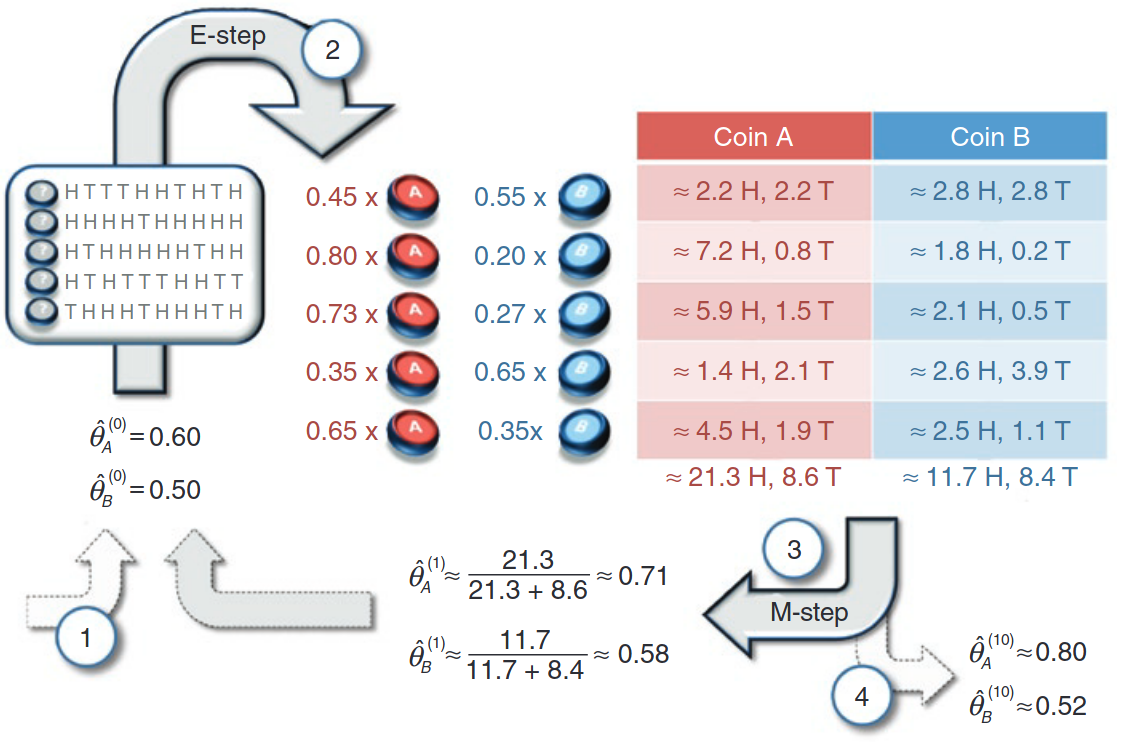
\includegraphics[width=0.7\textwidth]{tex/images/mixture}
  \caption{EM algorithm step in Mixture~\cite{do2008expectation}}\label{fig:mixture}
\end{figure}

We are know using the figure~\ref{fig:mixture} to set the example in a numerical context. We are following the given data points in the diagram.
\begin{enumerate}
  \item We are considering a prior \(\bm{\theta} = (0.6, 0.5)\), a set of \(N = 5\) samples and \(M = 10\) flips per sample.
  \item In the \textbf{E-step}, we calculate each \(Q(z_{n})\).
    \[
    \begin{aligned}
      Q(z_{1} = A) &= \frac{0.6^{5} 0.4^{5}}{0.6^{5}0.4^{5} + 0.5^{5}0.5^{5}} \approx 0.45 \implies Q(z_{1} = B) \approx 0.55,\\
      &\mathrel{\makebox[\widthof{=}]{\vdots}} \\
      Q(z_{5} = A) &\approx 0.65 \implies Q(z_{5}=B) \approx 0.35.
    \end{aligned}
    \]
  \item The \textbf{M-step} is then:
    \[
    \begin{aligned}
      \theta_{A} &= \sum_{n=1}^{5}Q(z_{n})\frac{x_{n}}{10} \approx \frac{21.3}{21.3 + 8.6} \approx 0.71,\\
      \theta_{B} &\approx 0.58.
    \end{aligned}
    \]
  \item Step 4 represents a possible solution after \(10\) iterations.
\end{enumerate}


\section{Partial steps}

Making a partial M-step consist on not using the optimal parameter for the energy term, but using one with just higher energy. Finding this values can be easier than finding the optimal one and convergence still follows as the only requirement to make the likelihood increase was to increase the lower bound.

On the other hand, when studying the increase on the likelihood, we supposed that the optimal E-step was being used. It cannot be guarantee that a partial step would increase the likelihood in this case, even though it does increase the lower bound.

Another important factor is, that the EM algorithm assumes that the energy term is possible to calculate, which may not be. As an approach to solve this situation, we can set a class of distributions \(\mathcal{Q}\), and minimize the Kullback-Leibler divergence between \(P(\bz \mid \bx, \theta)\) and a distribution \(Q \in \mathcal{Q}\), so we pick a distribution such that
\[
  Q = \argmin_{Q \in \mathcal{Q}} \KL{Q(\bz)}{P(\bz\mid \bx, \theta)}.
\]

An extreme case is to choose \(\mathcal{Q}\) as delta functions, where the energy term is now a constant, and the optimal setting is
\[
Q(z_{n}) = \delta (z_{n}, z_{n}^{opt}) \quad \text{and} \quad z_{n}^{opt} = \argmax_{z}P(z , x_{n} \mid \theta).
\]
This is called \emph{Viterbi training} and does not guarantee that the log likelihood is being increased on each iteration.

Viterbi training justifies its approach reasoning that, given the sufficient amount of data, the likelihood function \(P(\bx, \bz \mid \btheta)\) will be peaked around its optimum value. This suggest that the initial value of the parameter plays a major role in Viterbi training, compared to the classical EM. This technique is commonly used for training hidden Markov models (HMMs) (\cite{barber} Section 23.2).


\chapter{Mean-Field Variational Inference}
\section{The mean-field variational family}

The \emph{mean-field variational family} \(\mathcal{Q}\) is defined as the family of distributions where the variables are mutually independent, i.e, any \(Q \in \mathcal{Q}\) verifies
\[
  Q(\bz) = \prod_{m=1}^{M}Q_{m}(z_{m}),
\]

where \(\bZ = \{Z_{1},\dots,Z_{M}\}\) is the considered set of variables. The mean-field family is commonly used to model the family of distributions over the latent variables in our optimization problem. Notice that each \emph{factor} \(Q_{m}\) can be different and this family does not depend on the observed data.

The mean-field family can capture any marginal of the latent variables but not correlation between them, as it assumes they are independent. For example, consider a two dimensional Gaussian distribution where a high percentage of the density is inside the blue ellipse shown in Figure~\ref{fig:mean_field}. Any mean-field approximation would factorize as a product of two Gaussian distributions, condensing its density in a circle as shown in purple.

\begin{figure}[h!]
\centering
\begin{tikzpicture}
  \pgfplotsset{ticks=none}
    \begin{axis}[
        axis lines = middle,
        xmin=-11, xmax=11, ymin=-11, ymax=11,
        axis equal,
        xlabel = $z_{1}$,
        ylabel = {$z_{2}$},
        yticklabels={,,},
        ]
        \filldraw[rotate around={45:(110,110)}, color=blue!50, fill=blue!20, very thick, opacity=0.7] (110,110) ellipse (70 and 20);
        % \addlegendentry{Exact Posterior}
        \filldraw[color=purple!50, fill=purple!20, very thick, opacity=0.7]  (110,110) circle (25);
        % \addlegendentry{Mean-field Approximation}
    \end{axis}
  \end{tikzpicture}
  \caption{Mean-field family distribution (purple) approximating a Gaussian distribution (blue).}\label{fig:mean_field}
\end{figure}

Notice the parametric form of each factor \(Q_{m}\) is not specified and the appropriate configuration depends on the variable. For example, a continuous variable might have a Gaussian factor and a categorical variable have a categorical factor.

\section{CAVI algorithm }

In this section, we describe a widely used algorithm to solve the optimization problem we discussed in the previous section using the mean-field family. It is \emph{coordinate ascent variational inference} or \emph{CAVI} (also known as \emph{Variational Bayes}) and its procedure is to iteratively optimize each factor of the mean-field family distribution, while fixing the others. With this, the ELBO reaches a local optimum.

The \emph{coordinate ascent} approach is similar to the \emph{gradient ascent} in that both attempt to reach a local optima following a iterative procedure and maximizing each step. They differ in that the former updates each \emph{coordinate} (variable in this context) whereas the latter updates all of them using the direction of the gradient.

CAVI might be seen as a generalization of the EM algorithm, where the algorithm is extended to a full Bayesian approach, considering the parameters as latent variables. This will be reviewed in Section~\ref{sec:CAVI_EM}.

 \begin{algorithm}[t]
  \SetAlgoLined\KwData{A distribution \(P(\bx , \bm{z})\) with a dataset \(\bx\).}
  \KwResult{A distribution of the mean-field family \(Q(\bm{z}) = \prod_{m=1}^{M}Q_{m}(z_{m})\)}
  Initialize \(Q(\bm{z})\)\;
  \While{Convergence stop criteria}{
    \For{\(m \in 1,\dots,M\)}{
      \(\bm{z}_{\backslash m} = (z_{1},\dots,z_{m-1},z_{m+1},\dots,z_{M})\)\;
      Set \(Q_{m}(z_{m}) \propto \exp{\E{Q_{\backslash m}}{\log{P(z_{m} \mid \bm{z}_{\backslash m}, \bx)}}}\)\;
    }
    Compute \(ELBO(Q)\)\tcp*{Used for convergence criteria.}
  }
  \KwRet{\(Q\)}\;
  \caption{Coordinate Ascent Variational Inference}\label{alg:cavi}
\end{algorithm}


Let \(\bx\) be the given observations of the observed variables. CAVI iterates fixing all hidden variable but one at a time and maximizing its contribution to the ELBO. Consider the \(m^{th}\) variable \(Z_{m}\), denoting by \(\backslash m\) full set of indexes without the \(m^{th}\), then \(\bm{Z}_{\backslash m}\) is the full set of variables without the focused one. Let the factors \(Q_{n}, n\neq m\) be fixed.

The contribution of \(Z_{m}\) to the ELBO is (summarizing other factors in the constant term):
\[
  \begin{aligned}
    ELBO(Q) &= \E{Q}{\log{P(\bx, \bz)}} - \E{Q}{\log{Q(\bz)}}\\
    &\stackrel{1}{=} \E{Q_{m}}{\E{Q_{\backslash m}}{\log{P(\bx, \bm{z})}}} - \E{Q_{m}}{\log{Q_{m}(z_{m})}} + \text{ const. }\\
    &\stackrel{2}{=} \E{Q_{m}}{\E{Q_{\backslash m}}{\log{P(z_{m} \mid \bm{z}_{\backslash m}, \bx)} + \log{P(\bm{z}_{\backslash m}, \bx)}}} - \E{Q_{m}}{\log{Q_{m}(z_{m})}} + \text{ const. }\\
    &\stackrel{3}{=}  \E{Q_{m}}{\E{Q_{\backslash m}}{\log{P(z_{m} \mid \bm{z}_{\backslash m}, \bx)}}} - \E{Q_{m}}{\log{Q_{m}(z_{m})}} + \text{ const. }\\
    &\stackrel{4}{=} - \KL{Q_{m}(z_{m})}{  \exp{\E{Q_{\backslash m}}{\log{P(z_{m} \mid \bm{z}_{\backslash m}, \bx)}}} } + \text{ const.}.
  \end{aligned}
\]

\begin{enumerate}
  \item The expectations in the ELBO formula are separated. The logarithm factorizes as \(\log Q(z) = \sum_{m=1}^M \log Q_m(z_m)\).  The constant term comes from \( \E{Q_{\backslash m}}{\log Q_{\backslash m}(z_{\backslash m})} \).
  \item \( P \) is separated as \( P(\bz, \bx) = P(z_m \mid \bz_{\backslash m}, \bx)P(\bz_{\backslash m}, \bx) \implies \log P(\bz, \bx) = \log P(z_m \mid \bz_{\backslash m}, \bx) + \log P(\bz_{\backslash m}, \bx)\).
  \item \( \E{Q_{m}}{\E{Q_{\backslash m}}{\log{P(\bm{z}_{\backslash m}, \bx)}}} = \E{Q_{\backslash m}}{\log{P(\bm{z}_{\backslash m}, \bx)}}\) is constant.
  \item Applied Kullback-Leibler definition.
\end{enumerate}

Maximizing the ELBO is equivalent to minimize the given Kullback-Leibler divergence and this divergence is zero when \(Q_{m}^{new}\) is:
\[
  Q_{m}^{new}(z_{m}) \propto \exp{\E{Q_{\backslash m}}{\log{P(z_{m} \mid \bm{z}_{\backslash m}, \bx)}}}.
\]

Notice that the proportionality restriction is enough to fully determine the distribution as its integral is normalized. Equivalently, the distribution is proportional to
\begin{equation}\label{eq:cavi_update}
    Q_{m}^{new}(z_{m}) \propto \exp{\E{Q_{\backslash m}}{\log{P(z_{m}, \bm{z}_{\backslash m}, \bx)}}}.
\end{equation}

As the ELBO is generally a non-convex function and the CAVI algorithm converges to a local optimum, the initialization values of the algorithm play an important role on its performance. The convergence criteria is usually a threshold for the ELBO or a fixed amount of iterations.

\section{CAVI as an EM generalization}\label{sec:CAVI_EM}

As CAVI considers parameters as hidden variables, we need to specify a variational distribution for them. We are choosing the distribution that summarizes the information in the optimal point, let \(\btheta_{opt}\) be the optimal value of \(\btheta\):
\[
  Q(\btheta) = \delta(\btheta - \btheta_{opt}).
\]
The variational distribution factorizes as
\[
  Q(\bz, \btheta) = Q(\bz)Q(\btheta).
\]
The lower bound takes the form
\[
  \begin{aligned}
    \log{P(\bx \mid \btheta)} &\geq \E{Q(\bz, \btheta)}{\log{P(\bx, \bz, \theta)}} - \E{Q(\bz, \btheta)}{\log{Q(\bz, \btheta)}} \\
    &= \E{Q(\bz)}{\E{Q(\btheta)}{\log{P(\bx, \bz, \btheta)}}} - \E{Q(\bz)}{\log{Q(\bz)}} - \E{Q(\btheta)}{\log{Q(\btheta)}} \\
    &= \E{Q(\bz)}{\log{P(\bx, \bz, \btheta_{opt})}} - \E{Q(\bz)}{\log{Q(\bz)}} + \text{ const. }
  \end{aligned}
\]
The CAVI update can be seen as an iterative two step process. Firstly, given a fixed \(Q(\bz)\), as the distribution class of \(Q(\btheta)\) is fixed, optimizing it is equivalent to find the optimal parameter \(\btheta_{opt}\). 
\[
  \begin{aligned}
    \btheta_{opt} &= \argmax_{\btheta} \Big( \E{Q(\bz)}{\log{P(\bx,\bz,\btheta)}} \Big)\\
    &=  \argmax_{\btheta} \Big( \E{Q(\bz)}{\log{P(\bx, \bz \mid \btheta)P(\btheta)}} \Big) \\
    &= \argmax_{\btheta} \Big( \E{Q(\bz)}{\log{P(\bx, \bz \mid \btheta)}} + \log{P(\btheta)} \Big). \\
  \end{aligned}
\]

If we take a flat prior, this term is equivalent to the M-step. Secondly, given a fixed parameter \(\btheta\), the update is
\[
  Q(\bz) \propto \exp \E{Q(\btheta)}{\log P(\bz \mid \bx, \btheta)} =  P(\bz \mid \bx, \btheta_{opt}),
\]
which is the E-step of the EM algorithm.


\chapter{Exponential Family}

The exponential family (\cite{koopman1936distributions}) is a parametric set of probability distributions of a certain form. This form is chosen based on some useful algebraic properties and generality, Appendix~\ref{ap:exp_fam} shows some examples of common distributions in the exponential family.

Let \(X\) be a random variable and \(\bm{\theta}\) a set of parameters. A family of distributions is said to belong the exponential family if its probability distribution has the form
\[
  P(x \mid \bm{\theta}) = h(x)\exp{\Big( \sum_{i=1}^{S} \eta_{i}(\bm{\theta})T_{i}(x) - \psi(\bm{\theta}) \Big)},
\]
where \(h(x)\), \(T_{i}(x)\), \(\eta_{i}(\bm{\theta})\) and \(\psi(\bm{\theta})\)  are known functions such that \(h\) is called a \emph{base measure}, \(\eta_{i}(\bm{\theta})\) are called the \emph{distribution parameters},  \(T_{i}(x)\) the \emph{test statistics} and \(\psi\) is the \emph{log normalizer} as it ensures logarithmic normalization due to
\[
  \begin{aligned}
    1 &= \int_{x}  h(x)\exp{\Big( \sum_{i=1}^{S} \eta_{i}(\bm{\theta})T_{i}(x) - \psi(\bm{\theta}) \Big)}\\
    &= \int_{x} e^{-\psi(\btheta)} h(x)\exp{\Big( \sum_{i=1}^{S} \eta_{i}(\bm{\theta})T_{i}(x) \Big)}\\
    &= e^{-\psi(\btheta)} \int_{x} h(x)\exp{\Big( \sum_{i=1}^{S} \eta_{i}(\bm{\theta})T_{i}(x) \Big)},
  \end{aligned}
\]
so \(\psi\) verifies
\[
      \psi(\bm{\theta}) = \log \int_{x} h(x) \exp \Big( \sum_{i=1}^{S} \eta_{i}(\bm{\theta})T_{i}(x) \Big).
\]

Naming \(\bm{\eta}\) and \(\bm{T}\) the corresponding vector functions, the parameters can always be transformed as \(\bm{\theta}^{new} = \bm{\eta}(\bm{\theta})\), in which case we say the distribution into its \emph{canonical form} (notice \(\psi\) has changed but we do not distinguish it from the previous one since it is fully determined by the other functions):
\[
  P(x \mid \bm{\theta}) = h(x) e^{\bm{\theta}^{T}\bm{T}(x) - \psi(\bm{\theta})}.
\]
In this form, it is easier to see that \(\bm{T}\) is the sufficient statistic for \(\btheta\). This is a consequence of \emph{Fisher–Neyman factorization theorem} which says that \textit{\(\bm{T}\) is sufficient for \(\btheta\)  if and only if the probability distribution \(P\)  can be factored into a product such that one factor, \(h\), does not depend on \(\btheta\)  and the other factor, which does depend on \(\btheta\), depends on \(x\)  only through \(\bm{T}\).}

An important property of the exponential family is that they have \emph{conjugate priors}, this is said when the posterior distribution is in the same probability distribution family as
the prior distribution, they are then called \emph{conjugate distributions}, and
the prior is called a \emph{conjugate prior} of the likelihood distribution. Appendix~\ref{ap:conj_distr} shows examples of conjugate distributions and their conjugate priors. Models with conjugate priors are usually called \emph{conditionally conjugate models}.

\begin{proposition}\label{prop:conj_prior}
  Let \(X\) be a random variable and \(\btheta\) a set of parameters. Suppose an exponential family likelihood:
  \[
    P(x \mid \btheta) = h(x)e^{\btheta^{T}\bm{T}(x) - \psi(\btheta)}.
  \]
  and prior with hyper-parameters \(\bm{\alpha}, \gamma\):
  \[
    P(\btheta \mid \bm{\alpha}, \gamma) \propto e^{\btheta^{T} \bm{\alpha} - \gamma \psi(\btheta)}.
  \]
  Then, the posterior is in the same parametric family as the prior with
  \[
    P(\btheta \mid \bx, \bm{\alpha}, \gamma) = P(\btheta \mid \bm{\alpha} + \bm{T}(x), \gamma + 1).
  \]
\end{proposition}
\begin{proof}
  \[
    P(\btheta \mid \bx, \bm{\alpha}, \gamma)  \propto P(x \mid \btheta)P(\btheta \mid \bm{\alpha}, \gamma) \propto \exp \Big( \btheta^{T}[\bm{\alpha} + \bm{T}(x)] - [\gamma + 1]\psi(\btheta) \Big).
  \]
\end{proof}


\section{Latent variable and conditionally conjugate models}

One important case of exponential family are \emph{latent variable models} or \emph{LVMs}. In this models, the following assumptions are made:
\begin{enumerate}\itemsep0.5em
  \item There set of i.i.d random variables \(\bX = (X_{1},\dots,X_{N})\) and a set of observations \(\bx = (x_{1}, \dots, x_{N})\).
  \item There are both global and local latent variables. The global ones are denoted by \(\btheta\) whereas the locals are denoted by \(\bm{Z} = (Z_{1}, \dots, Z_{N})\). We refer to \emph{global hidden variables} when they affect the whole distribution and \emph{local hidden variables} when they affect only to a subset, in this case each \(Z_{n}\) affects only \(X_{n}\). Given this, the joint probability is
    \[
    P(\bx, \btheta, \bz) = P(\btheta)\prod_{n=1}^{N}P(z_{n}, x_{n} \mid \btheta).
    \]
  \item The \(n^{th}\) observation \(x_{n}\) and the \(n^{th}\) local hidden variable \(z_{n}\) are conditionally independent, given the global variables \(\btheta\), of all other observations and local hidden variables,
    \[
    P(x_{n},z_{n} \mid \btheta, \bx_{\backslash n}, \bz_{\backslash n}) = P(x_{n}, z_{n} \mid \btheta).
    \]
\end{enumerate}

\begin{remark}
  These models are widely used to discover patterns in data sets (\cite{blei2014build}).
  LVMs include popular models like \emph{Latent Dirichlet Allocation} models used to uncover the hidden topics in text corpora (\cite{blei2003latent}), mixture of Gaussian models to discover hidden clusters in data (\cite{bishop2006pattern}) and probabilistic principal component analysis for dimensionality reduction (\cite{tipping1999probabilistic}). These three models are reviewed throughout this document.
\end{remark}

One important case of LVMs and exponential family models are \emph{conditionally conjugate models} with local and global variables (\cite{blei2017variational}), where the following assumptions are made.
\begin{enumerate}[itemsep=2ex]
  \item The prior for the global latent variable \(P(\btheta)\) is in the exponential family with an hyper-parameter \(\alpha = [\alpha_{1}, \alpha_{2}]\), where \(\alpha_{1}\) is a vector and \(\alpha_{2}\) is a scalar, and statistics that concatenate the global latent variable \(\btheta\)  and its log normalizer from \(P(z_{n}, x_{n} \mid \btheta)\), \(\psi(\btheta)\)\footnote{The same symbol \(\psi\) is used for every normalizer function. The distinction must be made using their parameters. },
    \[
    P(\btheta) = h(\btheta) \exp \Big( \alpha^{T}[\btheta, -\psi(\btheta)] - \psi(\alpha)\Big).
    \]
  \item Each local term \(P(z_{n},x_{n} \mid \btheta)\) is in the exponential family of the form
    \[
    P(z_{n},x_{n} \mid \btheta) = h(z_{n}, x_{n}) \exp \Big( \btheta^{T} T(z_{n}, x_{n}) - \psi(\btheta) \Big).
    \]
  \item The complete conditional of a local latent variable verifies
    \[
    P(z_{n} \mid \btheta, \bx, \bz_{\backslash n}) = P(z_{n} \mid x_{n}, \btheta)
    \]
    and is also in the exponential family
    \[
    P(z_{n}\mid x_{n} , \btheta) =  h(z_{n})\exp \Big( {\eta(\btheta, x_{n})}^{T}T(z_{n}) - \psi(\btheta, x_{n}) \Big).
    \]
\end{enumerate}

Using Proposition~\ref{prop:conj_prior}, the posterior \(P(\btheta \mid \bx, \bz)\) is in the same family with parameter
\[
  \bar{\alpha} = {[\alpha_{1} + \sum_{n=1}^{N} T(z_{i}, x_{i}), \alpha_{2}+ N]}^{T}.
\]
A step by step reasoning would be:
\[
  \begin{aligned}
    P(\btheta \mid \bx, \bz) &= \frac{P(\bx, \bz \mid \btheta) P(\btheta)}{P(\bx, \bz)} \propto  P(\bx, \bz \mid \btheta) P(\btheta) = P(\btheta) \prod_{n=1}^{N}h(x_{n}, z_{n})\exp \Big( \btheta^{T}T(z_{n}, x_{n})  - \psi(\btheta) \Big)\\
    &\propto  h(\btheta) \exp \Big( \alpha^{T}[\btheta, -\psi(\btheta)]\Big)  \prod_{n=1}^{N}h(x_{n}, z_{n})\exp \Big( \btheta^{T}T(z_{n}, x_{n})  - \psi(\btheta) \Big)\\
    &\propto h(\btheta) \exp \Big(   \alpha^{T}[\btheta, -\psi(\btheta)] + \sum_{n=1}^{N}  \btheta^{T}T(z_{n}, x_{n})  - \psi(\btheta)  \Big)\\
    &\propto h(\btheta) \exp \Big(   \alpha_{1}^{T}\btheta  - \alpha_{2}^{T}\psi(\btheta) - N\psi(\btheta) + \sum_{n=1}^{N}  T(z_{n}, x_{n})^{T}\btheta  \Big)\\
    &\propto h(\btheta) \exp \Big(   \big(\alpha_{1} + \sum_{n=1}^{N}  T(z_{n}, x_{n})\big)^{T} \btheta  - (\alpha_{2} + N)^{T}\psi(\btheta) \Big).
  \end{aligned}
\]

\section{CAVI in conditionally conjugate models}~\label{sec:cavi_ccm}

Consider the following situation where we fit a distribution \(Q(\bm{z}) = \prod_{n=1}^{N} Q_{n}(z_{n})\) in the mean-field family, using an exponential family distribution for the marginal \(P(z_{n} \mid \bm{z}_{\backslash n}, \bx)\):
\[
  P(z_{n} \mid \bm{z}_{\backslash n}, \bx) = h(z_{n})\exp \Big( {\eta_{n}(\bm{z}_{\backslash n}, \bx)}^{T}T(z_{n}) - \psi(\bm{z}_{\backslash n}, \bx) \Big).
\]

The update of the CAVI algorithm  is then given by
  \begin{align}
    Q(z_{n}) &\propto \exp{\E{Q(\bm{z}_{\backslash n})}{\log P(z_{n} \mid \bm{z}_{\backslash n}, \bx)}} \nonumber\\
    &= h(z_{n})\exp \Big(\E{Q_{\bm{z}_{\backslash n}}}{ {\eta_{n}(\bm{z}_{\backslash n}, \bx)}}^{T}T(z_{n}) - \E{Q_{\bm{z}_{\backslash n}}}{ \psi(\bm{z}_{\backslash n}, \bx)}\Big) \nonumber \\
    &\propto  h(z_{n})\exp \Big(\E{Q_{\bm{z}_{\backslash n}}}{ {\eta_{n}(\bm{z}_{\backslash n}, \bx)}}^{T}T(z_{n})\Big) = h(z_{n})e^{v_{n}^{T}T(z_{n}) }, \label{eq:exponential_update}
  \end{align}

where
\[
  v_{n} = \E{Q_{\bm{z}_{\backslash n}}}{\eta_{n}(\bm{z}_{\backslash n}, \bx)}.
\]

Summarizing, the factor is in the exponential family with the same base measure \(h\) and updating it is equivalent to setting the distribution parameter \(\eta\) to the expected one of the complete conditional \(\E{}{\eta_{n}(\bx, \bm{z}_{\backslash n})}\). This expression facilitates deriving CAVI algorithm for many complex models.

Going back to the conditionally conjugate models, our variational distribution is in the mean-field family with \(Q(\btheta \mid \lambda)\) where \(\lambda\) is called the \emph{global variational parameter}, and for each local variable, the distribution is \(Q(z_{n} \mid \gamma_{n})\), where \(\gamma_{n}\) is called a \emph{local variational parameter}:
\[
  Q(z_{n} \mid \gamma_{n}) \propto h(z_{n})e^{{\gamma_{n}}^{T}T(z_{n})},
\]
\[
  Q(\btheta \mid \lambda) = h(\btheta) \exp \Big( {\lambda}^{T}[\btheta, -\psi(\btheta)] - \psi(\lambda) \Big).
\]

CAVI iteratively updates each local variational parameter and the global variational parameter.

Following the steps done in~\ref{eq:exponential_update}, the local variational parameter update is
\[
  \gamma_{n}^{new} = \E{Q(\btheta \mid \lambda)}{\eta(\btheta, x_{n})},
\]
In this case, the local hidden variable conditional does not depend on the other local hidden variables, neither other data-points.

The global variational parameter update is calculated as
\[
  \begin{aligned}
    Q^{new}(\btheta \mid \lambda) &\propto \exp \E{Q(\bz)}{\log P(\btheta \mid \bz , \bx)} \propto h(\btheta) \exp \E{Q(\bz)}{\big[  \lambda_{1} + \sum_{n=1}^{N}T(x_{n}, z_{n}), \lambda_{2} + N \big]^{T}\big[ \btheta, \psi(\btheta) \big]}\\
    &\propto h(\btheta) \exp \Bigg( {\Big[  \lambda_{1} + \sum_{n=1}^{N}\E{Q(\bz)}{T(x_{n}, z_{n})}, \lambda_{2} + N \Big]}^{T}\Big[ \btheta, - \psi(\btheta) \Big]\Bigg)\\
    &= Q(\btheta, \lambda^{new}).
  \end{aligned}
\]
Then, the variational parameter updated is
\[
  \lambda^{new} = \Bigg[ \lambda_{1} + \sum_{n=1}^{N} \E{Q(z_{n}\mid \gamma_{n})}{T(x_{n},z_{n})}, \lambda_{2} + N \Bigg].
\]

The ELBO can be computed at each iteration up to a constant which does not depend on the variational parameters,
\[
  \begin{aligned}
    ELBO &= {\Big( \lambda_{1} + \sum_{n=1}^{N} \E{Q(z_{n}\mid \gamma_{n})}{T(x_{n},z_{n})}\Big)}^{T}\E{Q(\btheta \mid \lambda)}{\btheta} - (\lambda_{2} + N) \E{Q(\btheta \mid \lambda)}{\psi(\btheta)}\\
    &+ \lambda ^{T} \E{Q(\btheta, \lambda)}{T(\btheta)} - \psi(\lambda) + \sum_{n=1}^{N}\gamma_{n}^{T}\E{Q(z_{n}, \gamma_{n})}{z_{n}} - \psi(\gamma_{n}) + \text{ const. }
  \end{aligned}
\]
The calculations are the following:
\[
  \begin{aligned}
   ELBO(Q(\btheta, \bz)) &= \E{Q(\btheta, \bz)}{\log{P(\btheta, \bz, \bx)}} - \E{Q(\btheta, \bz)}{\log{Q(\btheta, \bz)}}\\
  &= \E{Q(\bz \mid \bm{\gamma})}{\E{Q(\btheta \mid \lambda)}{\log P(\btheta, \bz, \bx)}}- \E{Q(\btheta, \bz)}{\log{Q(\btheta, \bz)}}\\
  &= \E{Q(\btheta \mid \lambda)}{\log P(\btheta)} + \E{Q(\bz \mid \bm{\gamma})}{\E{Q(\btheta \mid \lambda)}{\sum_{n=1}^{N} \log P(z_{n}, x_{n} \mid \btheta)}}\\
  &- \E{Q(\btheta, \bz)}{\log{Q(\btheta, \bz)}}
  \end{aligned}
\]
The first term is
\[
  \begin{aligned}
  \E{Q(\btheta \mid \lambda)}{\log P(\btheta)} &=  \E{Q(\btheta \mid \lambda)}{ \lambda_{1}\btheta - \lambda_{2}\psi(\btheta) - \psi(\lambda) }\\
  &= \lambda_{1}  \E{Q(\btheta \mid \lambda)}{\btheta} - \lambda_{2}\E{Q(\btheta \mid \lambda)}{\psi(\btheta)} - \psi(\lambda).
  \end{aligned}
\]
The middle term is 
\[
 \begin{aligned}
    &\E{Q(\bz \mid \bm{\gamma})}{\E{Q(\btheta \mid \lambda)}{\log P(\btheta, \bz, \bx)}} =  \E{Q(\bz \mid \bm{\gamma})}{\E{Q(\btheta \mid \lambda)}{\log P(\btheta) + \sum_{n=1}^{N} \log P(z_{n}, x_{n} \mid \btheta)}}\\
    &= \E{Q(\bz \mid \bm{\gamma})}{\E{Q(\btheta \mid \lambda)}{\log P(\btheta)}} + \E{Q(\bz \mid \bm{\gamma})}{\E{Q(\btheta \mid \lambda)}{\sum_{n=1}^{N} \log P(z_{n}, x_{n} \mid \btheta)}}\\
    &= {\Big( \lambda_{1} + \sum_{n=1}^{N} \E{Q(z_{n}\mid \gamma_{n})}{T(x_{n},z_{n})}\Big)}^{T}\E{Q(\btheta \mid \lambda)}{\btheta} - (\lambda_{2} + N) \E{Q(\btheta \mid \lambda)}{\eta(\btheta)}.
 \end{aligned}
\]
The last term is
\[
  \begin{aligned}
  \E{Q(\btheta, \bz)}{\log{Q(\btheta, \bz)}}  &= \E{Q(\btheta)}{\log Q(\btheta)} +  \E{Q(\bz)}{ \sum_{n=1}^{N} \log Q(z_{n})}\\
  &= \E{Q(\btheta)}{\lambda^{T}T(\btheta) - \psi(\lambda)} + \sum_{n=1}^{N} \E{Q(z_{n})}{\gamma_{n}^{T}z_{n} - \psi(\gamma_{n})}\\
  &= \lambda ^{T} \E{Q(\btheta, \lambda)}{T(\btheta)} - \psi(\lambda) + \sum_{n=1}^{N}\gamma_{n}^{T}\E{Q(z_{n}, \gamma_{n})}{z_{n}} - \psi(\gamma_{n}).
  \end{aligned}
\]



\chapter{Example: Gaussian Mixture}\label{ch:gm}
\section{Model statement}

A \emph{Gaussian mixture model} is a latent variable model where the data is assumed to be generated from a finite number of Gaussian distributions with unknown parameters.

\pgfmathdeclarefunction{gauss}{2}{%
  \pgfmathparse{1/(#2*sqrt(2*pi))*exp(-((x-#1)^2)/(2*#2^2))}%
}
\begin{figure}[h!]
  \centering
  \begin{tikzpicture}
    \begin{axis}[every axis plot post/.append style={
        mark=none,domain=-2:5,samples=50,smooth}, % All plots: from -2:2, 50 samples, smooth, no marks
      axis x line*=bottom, % no box around the plot, only x and y axis
      axis y line*=left, % the * suppresses the arrow tips
      enlargelimits=upper] % extend the axes a bit to the right and top
      \addplot {gauss(0,0.5)};
      \addplot {gauss(2,0.75)};
      \addplot {gauss(3, 0.4)};
    \end{axis}
  \end{tikzpicture}
  \caption{One-dimensional Gaussian mixture with three clusters. Those are \(\mathcal{N}(0, 0.5)\), \(\mathcal{N}(2, 0.75)\) and \(\mathcal{N}(3, 0.4)\).}
\end{figure}


The following elements are being considered (using~\cite{bishop2006pattern} Chapter 10.2 notation):
\begin{itemize}\setlength\itemsep{1em}
  \item \(K\) mixture components and \(N\) observations.
  \item A set of i.i.d \(\mathbb{R}^{D}\)-valued random variables \(\bX = (X_{1},\dots, X_{N})\) and a corresponding set of observations \(\bx = (x_{1},\dots, x_{n})\).
  \item The cluster assignment i.i.d latent variables \(\bZ = (Z_{1}, \dots, Z_{N})\), where each \(z_{n}\) is a binary vector where only one component is non zero, indicating the cluster to which \( x_n \) belongs.
  \item We choose a Dirichlet distribution over the mixing coefficients \(\bm{\pi}\)
    \[
    \bm{\pi} \sim \text{Symmetric-Dirichlet}(\alpha_{0}) \implies P(\bm{\pi}) \propto \prod_{k=1}^{K}\pi_{k}^{\alpha_{0}-1}.
    \]
    The hyper-parameter \(\alpha_{0}\) is the effective prior of each mixture component. Then \(\bm{\pi} = (\pi_{1},\dots,\pi_{K})\) are the mixture weights, i.e, prior probability of a particular component \(k\).
    \[
    P(\bz\mid \bm{\pi}) = \prod_{n=1}^{N}\prod_{k=1}^{K}\pi_{k}^{z_{n,k}} \implies Z_{n} \mid \bm{\pi} \sim \text{Categorical}(\bm{\pi}).
    \]
  \item The distribution mean and precision of each Gaussian distribution, \(\bm{\mu} = (\mu_{1},\dots,\mu_{K})\) and \(\bm{\Lambda} = (\Lambda_{1},\dots,\Lambda_{K})\),
    \[
    P(\bx \mid \bz, \bm{\mu}, \bm{\Lambda}) = \prod_{n=1}^{N}\prod_{k=1}^{K}\mathcal{N}{(\mu_{k}, \Lambda_{k}^{-1})}^{z_{n,k}}.\footnote{This notation symbolizes the density function of the given Gaussian distribution.}
    \]
  \item The prior governing \(\bm{\mu}\) and \(\bm{\Lambda}\) is an independent Gaussian-Wishart distribution with hyper parameters \(m_{0}, \beta_{0}, W_{0}\) and \(\nu_{0}\):
    \[
    P(\bm{\mu}, \bm{\Lambda}) = P(\bm{\mu} \mid \bm{\Lambda})P(\bm{\Lambda}) = \prod_{k=1}^{K}P(\mu_{k}\mid \Lambda_{k})P(\Lambda_{k})= \prod_{k=1}^{K}\mathcal{N}(m_{0}, {(\beta_{0}\Lambda_{k})}^{-1}) \mathcal{W}(W_{0}, \nu_{0}).
    \]
\end{itemize}

The joint probability factorizes as
\[
  P(\bm{x}, \bm{z}, \bm{\pi}, \bm{\mu}, \bm{\Lambda}) = P(\bm{x}\mid \bm{z}, \bm{\mu}, \bm{\Lambda})P(\bm{z}\mid \bm{\pi})P(\bm{\pi})P(\bm{\mu}\mid \bm{\Lambda})P(\bm{\Lambda}).
\]

The model can be represented with a Bayesian network as done in Chapter~\ref{ch:lvm_gm}. The needed steps to give the explicit CAVI update are now summarized following~\cite{bishop2006pattern}.

\section{Variational distribution and CAVI update}

We consider a variational distribution which factorizes as
\[
  Q(\bz, \bpi, \bmu, \bLambda) = Q(\bz)Q(\bpi, \bmu, \bLambda).
\]
Let us consider the update for \(Q(\bz)\), the update might be written as the following (using the explicit update given in~\ref{eq:cavi_update}):
\[
  Q^{new}(\bz) \propto \exp \E{Q(\bpi, \bmu, \bLambda)}{\log P(\bx, \bz, \bpi, \bmu, \bLambda)}.
\]
Which implies:
\[
  \begin{aligned}
    \log Q^{new}(\bz) &= \E{Q(\bpi, \bmu, \bLambda)}{\log P(\bx, \bz, \bpi, \bmu, \bLambda)} + \text{const.}\\
    &= \E{Q(\bpi, \bmu, \bLambda)}{\log \Big( P(\bx \mid \bz, \bmu, \bLambda)P(\bz \mid \bpi)P(\bpi)P(\bmu \mid \bLambda)P(\bLambda) \Big)} + \text{const.}\\
    &= \E{Q(\bpi)}{\log P(\bz \mid \bpi)} + \E{Q(\bmu, \bLambda)}{\log P(\bx \mid \bz, \bmu, \bLambda)} + \text{const.}
  \end{aligned}
\]
The first term is,
\[
  \begin{aligned}
    \E{Q(\bpi)}{\log P(\bz \mid \bpi)} &=  \E{Q(\bpi)}{\log \prod_{n=1}^{N}\prod_{k=1}^{K}\pi_{k}^{z_{n,k}}} = \E{Q(\bpi)}{\sum_{n=1}^{N}\sum_{k=1}^{K}z_{n,k}\log \pi_{k}}\\
    &= \sum_{n=1}^{N}\sum_{k=1}^{K}z_{n,k} \E{Q(\bpi)}{\log \pi_{k}}.
  \end{aligned}
\]
On the other hand, the latter is,
\[
    \begin{aligned}
    \E{Q(\bmu, \bLambda)}{\log& P(\bx \mid \bz, \bmu, \bLambda)} =\\
    &=  \E{Q(\bmu, \bLambda)}{\log \prod_{n=1}^{N}\prod_{k=1}^{K} \frac{1}{\sqrt{(2\pi)^{D}|\Lambda_{k}^{-1}|}} \exp \Big( -\frac{1}{2}{(x_{n} - \mu_{k})}^{T}\Lambda_{k}(x_{n}- \mu_{k}) \Big)  }\\
    &=  \E{Q(\bmu, \bLambda)}{ \sum_{n=1}^{N}\sum_{k=1}^{K}- \frac{D}{2}\log (2\pi)+  \frac{1}{2}\log |\Lambda_{k}|+ \Big( -\frac{1}{2}{(x_{n} - \mu_{k})}^{T}\Lambda_{k}(x_{n}- \mu_{k}) \Big)  }\\
    &=  \sum_{n=1}^{N}\sum_{k=1}^{K}  - \frac{D}{2} \log (2\pi)+ \frac{1}{2}\E{Q(\bLambda)}{\log |\Lambda_{k}|}- \frac{1}{2}\E{Q(\mu_{k}, \Lambda_{k})}{(x_{n} - \mu_{k})^{T}\Lambda_{k}(x_{n} - \mu_{k})}.
    \end{aligned}
\]
Given this, the new variational distribution \(Q^{new}(\bz)\) follows a Categorical distribution with parameters \(r_{n,k}\), which are the normalization of \(\rho_{n,k}\), defined as,
\[
  \log \rho_{n,k} = \E{Q(\bpi)}{\pi_{k}} + \frac{1}{2}\E{\bLambda}{\log | \Lambda_{k}|} - \frac{D}{2} \log (2\pi) - \frac{1}{2}\E{Q(\mu_{k}, \Lambda_{k})}{(x_{n} - \mu_{k})^{T}\Lambda_{k}(x_{n} - \mu_{k})},
\]
\[
  r_{n,k} = \frac{\rho_{n,k}}{\sum_{k=1}^{K}\rho_{n,k}}.
\]
Notice that, as \(\rho_{n,k}\) is defined as the exponential of a real value, it is positive. Therefore, \(r_{n,k}\) are non-negative and sum one as required.
The distribution is then
\[
  Q^{new}(\bz) = \prod_{n=1}^{N}\prod_{k=1}^{K} r_{n,k}^{z_{n,k}}.
\]
Using a similar reasoning to the factor \(Q(\bpi, \bmu, \bLambda)\), the update is:
\[
  \begin{aligned}
    \log Q^{new}(\bpi, \bmu, \bLambda) &= \E{Q(\bz)}{\log P(\bx, \bz, \bpi, \bmu, \bLambda)} + \text{const.}\\
    &=  \E{Q(\bz)}{\log \big( P(\bx \mid \bz, \bmu, \bLambda)P(\bz \mid \bpi)P(\bpi)P(\bmu \mid \bLambda)P(\bLambda) \big)} + \text{const.}\\
    &=  \log P(\bpi) + \log P(\bmu \mid \bLambda)+ \log P(\bLambda) + \E{Q(\bz)}{\log P(\bz \mid \bpi)} \\
    &\quad + \E{Q(\bz)}{\log P(\bx \mid \bz, \bmu, \bLambda)} + \text{const.}\\
    &= \log P(\bpi) + \sum_{k=1}^{K}\log P(\mu_{k}, \Lambda_{k}) + \E{Q(\bz)}{\log P(\bz \mid \bpi)}\\
    &\quad + \sum_{n=1}^{N}\sum_{k=1}^{K}r_{n,k} \log \mathcal{N}(\mu_{k}, \Lambda_{k}^{-1}) + \text{const.}
  \end{aligned}
\]
Where \(\E{\bz}{z_{n,k}} = r_{n,k}\) is used. The right term can be decomposed in terms involving only \(\bpi\) and each \(\mu_{k}, \Lambda_{k}\). Therefore, the variational distribution factorizes as
\[
  Q(\bpi, \bmu, \bLambda) = Q(\bpi)\prod_{k=1}^{K}Q(\mu_{k}, \Lambda_{k}).
\]
Where
\[
  \begin{aligned}
    \log Q^{new}(\bpi) &= \log P(\bpi) + \E{Q(\bz)}{\log P(\bz \mid \bpi)} + \text{const.}\\
    \log Q^{new}(\mu_{k}, \Lambda_{k}) &= \log P(\mu_{k}, \Lambda_{k}) + \sum_{n=1}^{N}r_{n,k} \log \mathcal{N}(\mu_{k}, \Lambda_{k}^{-1}) + \text{const.}
  \end{aligned}
\]
Inspecting the term that depends on \(\bpi\) one get that,
\[
  \log Q^{new}(\bpi) = (\alpha_{0} - 1)\sum_{k=1}^{K}\log \pi_{k} + \sum_{n=1}^{N}\sum_{k=1}^{K}r_{n,k} \log \pi_{k} + \text{const}.
\]
Naming \(N_{k} = \sum_{n=1}^{N}r_{n,k} \ \forall k=1,\dots,K\), the update is
\[
  Q^{new}(\bpi) \propto \prod_{k=1}^{K}\pi_{k}^{\alpha_{0}-1+N_{k}}.
\]
Defining \(\bm{\alpha}\), with components:
\[
  \alpha_{k} = \alpha_{0} + N_{k}, \quad \forall k = 1,\dots,K,
\]
the new variational distribution follows a Dirichlet distribution
\[
  Q^{new}(\bpi) \equiv \text{Dirichlet}(\bm{\alpha}).
\]
Lastly, the variational distribution \(Q(\mu_{k}, \Lambda_{k})\) does not factorize but the update is given by
\[
  \begin{aligned}
    \log Q^{new}(\mu_{k}, \Lambda_{k}) &= \log P(\mu_{k}, \Lambda_{k}) + \sum_{n=1}^{N}r_{n,k} \log \mathcal{N}(\mu_{k}, \Lambda_{k}^{-1}) + \text{const.}\\
    &= \log \mathcal{N}(m_{0}, {(\beta_{0}\Lambda_{k})}^{-1}) + \log \mathcal{W}(W_{0}, \nu_{0}) + \sum_{n=1}^{N}r_{n,k} \log \mathcal{N}(\mu_{k}, \Lambda_{k}^{-1}) + \text{const.}\\
    &= \frac{\beta_{0}}{2}{(\mu_{k} - m_{0})}^{T}\Lambda_{k}(\mu_{k} - m_{0}) + \frac{1}{2}\log |\Lambda_{k}| - \frac{1}{2}Tr(\Lambda_{k}W_{0}^{-1})\\
    &\quad + \frac{\nu_{0} - D - 1}{2}\log |\Lambda_{k}| - \frac{1}{2}\sum_{n=1}^{N}r_{n,k}{(x_{n}- \mu_{k})}^{T}\Lambda_{k}(x_{n} - \mu_{k})\\
    &\quad + \frac{1}{2}N_{k} \log |\Lambda_{k}| + \text{const.}
    \end{aligned}
  \]
  Using Appendix~\ref{ap:G-GW}, the above formula is similar the posterior distribution of a Gaussian likelihood and Gaussian-Wishart prior. Using the procedure used in the appendix, the posterior follows a Gaussian-Wishart distribution with parameters:
  \[
    Q^{new}(\mu_{k}, \Lambda_{k}) \equiv  \mathcal{N}( m_{k}, (\beta_{k}\Lambda_{k})^{-1}) \mathcal{W}(W_{k}, \nu_{k}).
  \]
  Where,
  \[
    \begin{aligned}
      \beta_{k} &= \beta_{0} + N_{k},\\
      m_{k} &= \frac{1}{\beta_{k}}\Big(\beta_{0}m_{0} + \sum_{n=1}^{N}r_{n,k}x_{n}\Big),\\
      \bar{x}_{k} &= \frac{1}{N_{k}}\sum_{n=1}^{N}r_{n,k}x_{n},\\
      S_{k} &= \frac{1}{N_{k}}\sum_{n=1}^{N}r_{n,k}(x_{n}- \bar{x}_{k})(x_{n} - \bar{x}_{k})^{T},\\
      W_{k}^{-1} &= W_{0}^{-1} + N_{k}S_{k} + \frac{\beta_{0}N_{k}}{\beta_{0} + N_{k}}(\bar{x}_{k} - m_{0})(\bar{x}-m_{0})^{T},\\
      \nu_{k} &= \nu_{0} + N_{k}.
    \end{aligned}
  \]


\ctparttext{
  \color{black}
  \begin{center}

    A \emph{graphical model} is a statistical model for which the dependence structure between random variables is expressed by a graph.

    Commonly, they provide a graph-based representation for encoding a multi-dimensional
    distribution representing a set of independences that hold in the specific
    distribution. The most commonly used are \emph{Bayesian networks} and \emph{Markov random
      fields}, these two differ in the set of independences they are able to encode and the
    factorization of the distribution they include.
  \end{center}
}
\part{Graphical Models}

\chapter{Introduction}

\emph{Probabilistic graphical models} are diagrammatic representations of probability distributions that represent the dependence/independence relation between the considered variables. Their use presents the following advantages (\cite{bishop2006pattern}):
\begin{enumerate}\setlength{\itemsep}{0.2cm}
  \item They allow a simple visualization of probabilistic models.
  \item Insights into the model's properties can be obtained form the graph.
  \item Complex computations, required in inference task, are simplified using the graph structure.
\end{enumerate}

In probabilistic graphical models, each node represents a random variable and links represents relations between them. The graph encodes how the joint probability distribution of the considered variables factorizes. The different classes of graphical models differ in how they represent these relations and how the distribution is factorized.

We begin discussing \emph{Bayesian networks}, also known as \emph{directed graphical models}, where links between variables are indicated by a directed arrow.  The other major class of graphical models are \emph{Markov random fields} or \emph{undirected graphical models} in which links have no directional meaning. The former are useful to express casual relations between the variables whereas the latter express soft constraints between them.

Consider a set of variables \(\bX = (X_{1},\dots, X_{N})\), the possible ways these variables can interact is extremely large, for binary variables, the joint distribution table would take \(O(2^{N})\) space, which is unpractical when the amount of variables scales. When dealing with this such large distributions it is a common practice to factorize the joint probability in a graphical model, reducing the needed resources to deal with the inference problem.


\chapter{Bayesian networks}

Given a set of variables \(\bX = (X_{1},\dots,X_{N})\), \emph{Bayesian networks} might be defined either as a probability distribution of a certain form or a DAG whose nodes represent these variables and links an independence constraint. Both ideas are present in the following definition.

\begin{definition}
  A \emph{belief network or Bayesian network} is a pair \((G,P)\) formed by a DAG \(G\) and  joint probability distribution \(P\) such that, there is a correspondence between variables and nodes such as:
  \[
    P(x_{1},\dots,x_{N}) = \prod_{n=1}^{N}P(x_{n}\mid pa(x_{n})).
  \]
\end{definition}

\begin{remark}
  A Bayesian network might be given as a distribution from which the DAG can be constructed or a DAG which represents the distribution. For example in Figure~\ref{fig:bn_example}, given the DAG one could easily define the joint distribution and conversely.
\end{remark}

\begin{figure}[h!]
  \centering
  \begin{tikzpicture}[
    node distance=1.5cm and 1.5cm,
    mynode/.style={draw,circle,text width=0.5cm,align=center}
    ]

    \node[mynode] (1) {\(X_1\)};
    \node[mynode,right=of 1] (2) {\(X_2\)};
    \node[mynode,right=of 2] (3) {\(X_3\)};
    \node[mynode,right=of 3] (4) {\(X_4\)};

    \path (4) edge[-latex][bend right] (1)
    (3) edge[-latex] (2)
    (4) edge[-latex][bend right] (2)
    ;

    \end{tikzpicture}
    \captionof{figure}{Bayesian Network factorizing \(P(x_1, x_2, x_3, x_4) = P(x_1 \mid x_4)P(x_2\mid x_3, x_4)P(x_3)P(x_4)\)}\label{fig:bn_example}
\end{figure}

Any probability distribution can be written as a Bayesian Network, even though
it may end up being a fully-connected ``cascade''\footnote{This term comes from the visual structure of the graph.} DAG, which means that each variable \( X_n \) is a parent of any \( X_m \) with \( m > n \). This is because any distribution satisfies:
\[
   P(x_1, \dots, x_{N}) = P(x_1) \prod_{n=2}^{N}P(x_{n} \mid x_{1},\dots, x_{n-1})
 \]

Bayesian Networks are good for encoding \emph{conditional independence} over the
variables, but are not for encoding dependence. For example, with the following
network
\[
P(x,y) = P(y\mid x)P(x).
\]
represented as \(x \to y\) in a DAG, it may appear to encode dependence between both variables but the conditional \(P(y\mid x)\) could happen to equal \(P(y)\), giving \(P(x,y) = P(x)P(y)\).

How could we check if two variables are conditionally independent given a
Bayesian network? For example in Figure~\ref{fig:relations}, \(X_1 \bigCI
X_2 \mid X_4\) as
\[
\begin{aligned}
P(x_2 | x_4) &= \frac{1}{P(x_4)}\int_{x_1,x_3}P(x_1, x_2, x_3, x_4)
= \frac{1}{P(x_4)}\int_{x_1,x_3}P(x_1|x_4)P(x_2|x_3,x_4)P(x_3)P(x_4)\\
                 &= \int_{x_3}P(x_2|x_3, x_4)P(x_3),
\end{aligned}
\]
\[
\begin{aligned}
P(x_1, x_2 | x_4) &= \frac{1}{P(x_4)}\int_{x_3}P(x_1, x_2, x_3, x_4)
= \frac{1}{P(x_4)}\int_{x_3}P(x_1|x_4)P(x_2|x_3,x_4)P(x_3)P(x_4)\\
                 &= P(x_1|x_4)\int_{x_3}P(x_2|x_3, x_4)P(x_3) = P(x_1|x_4)P(x_2|x_4).
\end{aligned}
\]

\begin{proposition}\label{prop:bn_neig_indep}
  Let \(X\) and \(Y\) be two different nodes of a Bayesian network such as \(Y \not \in ne(X)\), then
  \[
    X \bigCI Y \mid ne(X).
  \]
  Which means that all information about \(X\) is in its neighbors.
\end{proposition}

\section{D-separation and D-connection}

Now we are going to define two central concepts to determine conditional
independence in any Bayesian network, these are \emph{d-connection} and \emph{d-separation}.

\begin{definition}
Let \(G\) be a DAG where \(\bm{X}, \bm{Y} \text{ and } \bm{Z}\)
are disjoint sets of vertices. We say that \(\bm{X} \text{ and
} \bm{Y}\) are \emph{d-connected} by \(\bm{Z}\) if and only if there
exists an undirected path \(U\) from any vertex in \(\bm{X}\) to any
vertex in \(\bm{Y}\) such that:
\begin{itemize}
\item For any collider \(C\), itself or any it's descendants is in \(\bm{Z}\).
\item No non-collider on \(U\) is on \(\bm{Z}\).
\end{itemize}
\end{definition}

\begin{definition}
Let \(G\) be a DAG where \(\bm{X}, \bm{Y} \text{ and } \bm{Z}\)
are disjoint sets of vertices. \(\bm{X}\) and \(\bm{Y}\)
are \emph{d-separated} by \(\bm{Z}\) if and only if they are not
d-connected by \(\bm{Z}\) in \(G\)
\end{definition}

\begin{figure}[t]
\centering
\begin{tikzpicture}[
  node distance=1cm and 0.5cm,
  mynode/.style={draw,circle,text width=0.5cm,align=center}
]

\node[mynode] (a) {a};
\node[mynode, below right=of a] (d) {d};
\node[mynode,above right=of d] (b) {b};
\node[mynode, below right=of b] (e) {e};
\node[mynode,above right=of e] (c) {c};

\path (a) edge[-latex] (d)
(b) edge[-latex] (d)
(c) edge[-latex] (e)
(b) edge[-latex] (e)
;

\end{tikzpicture}
\caption{D-separation example}\label{fig:d-sep}
\end{figure}

For example, in Figure~\ref{fig:d-sep}, \(d\) d-separates \(a\) and \(c\) (\(e\)
is a collider in the path that is not in \(\{d\}\)),
and \(\{d,e\}\) d-connect them.

\begin{theorem}[\cite{pearl_and_detcher}]\label{th:d-separation}
Let \(G\) be a DAG where \(\bm{X}, \bm{Y} \text{ and } \bm{Z}\)
are disjoint sets of vertices. If  \(\bm{X}\) and \(\bm{Y}\)
are d-separated by \(\bm{Z}\), then they are independent conditional
on \(\bm{Z}\) in all probability distributions that \(G\) may represent.
\end{theorem}

The Bayes Ball algorithm (\cite{bayes_ball}) provides a linear time complexity
algorithm that computes conditional independent using this theorem.


In cases where the Bayesian networks contains i.i.d nodes that are
essentially the same but repeated a number of times, the \emph{plate notation} is commonly used to represent this nodes in a compacted manner (Figure~\ref{fig:plate_notation}).

\begin{figure}[t]
\centering
\begin{tikzpicture}[
  node distance=1cm and 0.5cm,
  mynode/.style={draw,circle,text width=0.5cm,align=center}
]

\node[mynode] (a) {A};
\node[mynode,below=of a] (d) {\(B_3\)};
\node[mynode,left=of d] (c) {\(B_2\)};
\node[mynode,left=of c] (b) {\(B_1\)};
\node[mynode,right=of d] (e) {\(\dots\)};
\node[mynode,right=of e] (f) {\(B_n\)};

\node[mynode,right=2cm of f] (g) {\(B_i\)};
\node[mynode, above=of g] (h) {A};
\plate{} {(g)} {\(n\)}; %


\path (a) edge[-latex] (b)
(a) edge[-latex] (c)
(a) edge[-latex] (d)
(a) edge[-latex] (e)
(a) edge[-latex] (f)
(h) edge[-latex] (g)
;

\end{tikzpicture}
\caption{Plate notation example. Standard notation on the left and plate on the right.}\label{fig:plate_notation}
\end{figure}


\begin{exampleth}
In this example we are modeling three discrete random variables: Sprinkler (\(S\)),
Rain (\(R\)) and Grass wet (\(G\)).

The joint probability function is:
\[
P(s,r,g) = P(s|r)P(g|s,r)P(r)
\]

The following DAG illustrates the Bayesian network among with the probability
tables we are using.

\begin{figure}[ht]
\begin{tikzpicture}[
  node distance=0.6cm and 0cm,
  mynode/.style={draw,ellipse,text width=1.7cm,align=center}
]
\node[mynode] (sp) {Sprinkler};
\node[mynode,below right=of sp] (gw) {Grass wet};
\node[mynode,above right=of gw] (ra) {Rain};
\path (ra) edge[-latex] (sp)
(sp) edge[-latex] (gw)
(gw) edge[latex-] (ra);
\node[left=0.5cm of sp]
{
\begin{tabular}{cm{1cm}m{1cm}}
\toprule
& \multicolumn{2}{c}{Sprinkler} \\
Rain & \multicolumn{1}{c}{T} & \multicolumn{1}{c}{F} \\
\cmidrule(r){1-1}\cmidrule(l){2-3}
F & 0.4 & 0.6 \\
T & 0.01 & 0.99 \\
\bottomrule
\end{tabular}
};
\node[right=0.5cm of ra]
{
\begin{tabular}{m{1cm}m{1cm}}
\toprule
\multicolumn{2}{c}{Rain} \\
\multicolumn{1}{c}{T} & \multicolumn{1}{c}{F} \\
\cmidrule{1-2}
0.2 & 0.8 \\
\bottomrule
\end{tabular}
};
\node[below=0.5cm of gw]
{
\begin{tabular}{ccm{1cm}m{1cm}}
\toprule
& & \multicolumn{2}{c}{Grass wet} \\
\multicolumn{2}{l}{Sprinkler Rain} & \multicolumn{1}{c}{T} & \multicolumn{1}{c}{F} \\
\cmidrule(r){1-2}\cmidrule(l){3-4}
F & F & 0.0 & 1.0 \\
F & T & 0.8 & 0.2 \\
T & F & 0.9 & 0.1 \\
T & T & 0.99 & 0.01 \\
\bottomrule
\end{tabular}
};
\end{tikzpicture}
\end{figure}

This model can answer questions about the presence of a cause given the presence
of an effect. For example, What is the probability that it has being raining
given the grass is wet?

\[
P(R = T | G = T) = \frac{P(G = T, R = T)}{P(G=T)} = \frac{\sum_{s}P(G=T, R=T,
s)}{\sum_{r,s} P(G=T, r, s)}
\]

Using the expression of the joint probability among with the tables we can
compute every term. For example:
\[
\begin{aligned}
P(G=T, R=T, S=T) &= P(S=T|R=T)P(G=T|R=T,S=T)P(R=T) \\
&= 0.01 * 0.99 * 0.2 = 0.00198
\end{aligned}
\]
\end{exampleth}


\chapter{Markov Random Fields}

Whereas Bayesian networks are represented by an acyclic directed graph, \emph{Markov random fields} are undirected graphs that may be cyclic. Thus, this kind of graphical models are able to represent certain dependencies which Bayesian networks cannot, like cyclic ones. \emph{Markov random fields} are commonly used to model tasks in computer vision and image processing (\cite{li2009markov}).

\begin{definition}
  Given an undirected graph \(G = (V, E)\), a set of random variables \(\bX = (X_{1}, \dots, X_{N})\) \emph{form a Markov random field over \(G\)} if they satisfy the, so called, Markov properties (\cite{barber}):
  \begin{itemize}
  \item \textbf{Pairwise Markov property}. Any two non-adjacent variables are
      conditionally independent given all other variables:
      \[
      X_{n} \bigCI X_{m} \mid \bX_{\backslash n,m} \quad \forall n,m \in \{1,\dots,N\} \quad n \neq m.
      \]
    \item \textbf{Local Markov property}. Any variable is conditionally independent over all
    other variables given its neighbors:
    \[
      X_{n} \bigCI \bX_{\backslash ne(X_{n})} \mid \bX_{ne(X_{n})} \quad \forall n \in \{1,\dots,N\}.
      \]
  \item \textbf{Global Markov property}. Any two subsets of variables are conditionally
    independent given a separating subset (any path from one set to the other
      passes trough this one). Let \(A\) and \(B\) be two subset of indexes and \(S\) a separating subset:
      \[
      \bX_{A} \bigCI \bX_{B} \mid \bX_{S}.
      \]
  \end{itemize}

  The Global Markov property is stronger than the Local Markov property, which is stronger than the Pairwise one. However, these properties are equivalent for positive distributions (\(P(x) > 0\)), this is Theorem 4.4 in~\cite{koller_friedman}.
\end{definition}

As these Markov properties can be difficult to establish, a commonly used class of Markov random fields are those who factorize as product of potentials over the graph's cliques.

\begin{definition}
A \emph{potential} \(\phi\) is a non-negative function. It is worth to mention
that a probability distribution is a special case of a potential.
\end{definition}

Let \(\bm{X}\) be a set of random variables, \(G\) an undirected graph whose nodes are \(\bX\) and \(\bm{X}_c, c \in \{1,\dots,C\}\) be the maximal cliques of \(G\). If the joint probability distribution \(P\) can be factorized as:
\[
P(x_1,\dots,x_n) = \frac{1}{Z}\prod_{ c = 1 }^{C}\phi_c(\bm{X}_c).
\]
where \(Z\) is a constant that ensures normalization. Figure~\ref{fig:mn_example} shown an example in this class of Markov random fields.

Markov random fields factorize if any of the following conditions is fulfilled:
\begin{itemize}
  \item The distribution is positive, this is shown in Hammersley–Clifford theorem (\cite{grimmett1973theorem}).
  \item The graph is \emph{chordal}, which means that any cycle of four of more vertices has a chord, an edge that is not part of the cycle but connects two of its vertices.
\end{itemize}


\begin{figure}[h]
\centering
\begin{tikzpicture}[
  node distance=1cm and 1.5cm,
  mynode/.style={draw,circle,text width=0.5cm,align=center}
]

\node[mynode] (1) {\(X_1\)};
\node[mynode,right=of 1] (2) {\(X_2\)};
\node[mynode,below=of 1] (3) {\(X_3\)};
\node[mynode,right=of 3] (4) {\(X_4\)};
\path (1) edge (2)
(1) edge (3)
(2) edge (3)
(2) edge (4)
(1) edge (4)
;
\end{tikzpicture}
\captionof{figure}{Markov Network \(P(x_1, x_2, x_3, x_4) = \phi(x_1, x_2,
  x_3)\phi(x_2, x_3, x_4)/Z\)}
\label{fig:mn_example}
\end{figure}


\ctparttext{
  \color{black}
  \begin{center}
    Some inference methods get optimized when applied among with a graphical model. In this part we focus in how methods we have already reviewed use the Bayesian network structure to get simplified and optimized.

    The \emph{PC algorithm} is also reviewed as a procedure to generate a Bayesian network from a given dataset.

  \end{center}
}
\part{Bayesian Networks Parametric Learning}

\chapter{Structure Learning}

The Bayesian network structure is not always given and has to be learned from the data, to achieve this, there are some issues that need to be considered. These are:
\begin{itemize}\setlength{\itemsep}{0.15cm}
  \item The number of Bayesian networks is exponential over the number of variables so a brute force algorithm would not be viable.
  \item Testing dependencies requires a large amount of data, therefore, a threshold needs to be established to measure when a dependence is significant.
  \item The presence of hidden variables might not be learned from the data.
\end{itemize}


\begin{algorithm}[t]
  \SetAlgoLined\KwData{Complete undirected graph \(G\), with vertices \(V\)}
  \KwResult{\(G\) with removed links}
  \(i = 0\)\;
  \While{all nodes have \(\leq i\) neighbors}{
    \For{\(X \in V\)}{
      \For{\(Y \in ne(x)\)}{
        \If{\(\exists S \subset ne(X)\backslash Y\) such that \(\#S = i\) and
          \(X \bigCI Y \mid S\)}{
          Remove \(X-Y\) from \(G\)\;
          \(S_{XY} = S\)\;
        }
      }
    }
    \(i = i+1\)\;
  }
  \caption{PC Algorithm for skeleton learning}\label{alg:pc}
\end{algorithm}

\section{PC algorithm}

The \emph{PC algorithm} (\cite{spirtes2000causation} Chapter 5.4.2) learns the skeleton structure given a complete graph \(G=(V,E)\) (constructed from the considered set of variables) and orients its edges using variable independence in the empirical distribution. The following theorem provides the motivation for the algorithm's procedure.

\begin{theorem}[\cite{spirtes2000causation} Theorem 3.4]
  A distribution \(P\) is faithful to a directed acyclic graph \(G = (V,E)\)  if and only if
  \begin{itemize}
    \item two vertices \(X\) and \(Y\) are adjacent if and only if are dependent conditionally on every set of vertices that does not contain either of them, i.e,
      \[
      X \in ne(Y) \iff X \bigCD Y \mid S \quad \forall S \subset V \setminus \{X,Y\},
      \]
      and
    \item for any three vertices such that \(X \in ne(Y)\), \(Y \in ne(Z)\) and \(X \notin ne(Z)\),  \(X \to Y \leftarrow Z\) is in \(G\) if and only if \(X \bigCD Z \mid S\cup \{Y\} \ \forall S \subset V \setminus \{X,Z\}\).
  \end{itemize}

\end{theorem}

The \emph{PC algorithm} is split in two parts, firstly, the skeleton structure is learned, that is, given the complete graph, as many edges as possible are removed. This part (Algorithm~\ref{alg:pc}) iterates over subsets of neighborhoods, from smaller to bigger ones. It chooses a linked pair of variables \((X,Y) \in E\) and
a subset \(S_{XY} \subset ne(X)\), verifying \(Y \notin S_{XY}\). If \(X \bigCI Y \mid S_{XY}\), then the link is removed and \(S_{XY}\) is stored as their separation set.

The followed reasoning is: as \(X \bigCI Y \mid S_{XY}\) and \(S_{XY} \subset V \setminus \{X,Y\}\), the first part of the theorem ensures that \(X \notin ne(Y)\).

This procedure results in the skeleton of the Bayesian network, no more edges will be removed or added. The directed graph may be constructed following two rules:
\begin{enumerate}
  \item For any undirected link \(X - Y - Z\), if \(Y \notin S_{XZ}\) then set
    \(X \to Y \leftarrow Z\) (we are creating a collider for that path).
  \item The rest of links may oriented arbitrarily not
creating cycles or colliders.
\end{enumerate}
The reasoning behind is the d-separation Theorem~\ref{th:d-separation}, if \(Y \notin S_{XZ}\) then \(X \bigCD Z \mid Y\). Otherwise, they would be independent \(X \bigCI Z \mid Y\) and \(\{Y\}\) would be the d-separation set \(S_{XZ} = \{Y\}\) as they are checked from smaller to bigger ones. But \(Y \notin S_{XZ}\), therefore, using Theorem~\ref{th:d-separation}, \(Y\) must d-connect \(X\) and \(Y\), to achieve this, \(Y\)  must be set as a collider of the path. This is because, using the d-connection definition, the only known undirected path is \(U = X - Y - Z\) and no non-collider on \(U\) must belong to \(\{Y\}\).

Conversely, if \(Y \in S_{XZ}\) and \(X \bigCI Z \mid S_{XZ}\) then \(S_{XZ}\) should d-separate them, that is, using any configuration that does not create a collider in \(S_{XZ}\).

\section{Independence learning}

The PC algorithms assumes there exists a procedure of testing conditional independence of variables, that is, given three variables \(X, Y\) and \( Z \),  measure \(X \bigCI Y \mid Z\). One approach is to measure the empirical \emph{conditional mutual information} of the variables.

\begin{definition}
  Given two random variables \(X, Y\), we define their \emph{mutual information} as the Kullback-Leibler divergence of their joint distribution and the product of their marginals,
  \[
    MI(X;Y) = \KL{P_{X,Y}}{P_{X}P_{Y}}.
  \]
\end{definition}

\begin{definition}
  Given three random variables \(X, Y, Z\) we define the \emph{conditional mutual information} of \(X\) and \(Y\) over \(Z\) as
  \[
    MI(X;Y\mid Z) = \E{Z}{\KL{P_{X,Y \mid Z}}{P_{X\mid Z} P_{Y \mid Z}}}.
  \]
\end{definition}
Where \(MI(X;Y \mid Z) \geq 0\) and
\[
MI(X;Y \mid Z) = 0 \iff P_{X,Y \mid Z} = P_{X\mid Z} P_{Y \mid Z} \iff X\bigCI Y \mid Z.
\]
These values might be estimated using their empirical distributions, however, this \emph{empirical} mutual information will be typically greater than \(0\) even when \(X\bigCI Y \mid Z\). Thus, a threshold must be established. This is commonly done by using a statistical test, taking into consideration that the empirical mutual information follows a chi-squared distribution under independence (\cite{kullback1997information}).

A Bayesian approach would consist on comparing the model likelihood under independence and dependence hypothesis, let \((\bx, \by, \bz) = \{(x_{n}, y_{n}, z_{n})\}_{n=1,\dots, N}\) be the known data of each variable:
\[
  P_{indep}(\bx,\by,\bz) = \int_{\btheta} P(\btheta) \prod_{n=1}^{N} P(x_{n}\mid z_{n}, \btheta)P(y_{n} \mid z_{n}, \btheta)P(z_{n} \mid \btheta),
\]
\[
P_{dep}(\bx, \by, \bz) = \int_{\btheta} P(\btheta) \prod_{n=1}^{N}P(x_{n}, y_{n}, z_{n} \mid \btheta).
\]
Which means checking which assumptions is most probable to have generated the data.



\chapter{Maximum Likelihood Training}

Consider a set of i.i.d variables \(\bX = (X_{1},\dots,X_{N})\), when reviewing maximum likelihood training, we concluded that, in case \(P(x_{1},\dots, x_{N} \mid \theta)\) is unconstrained, the maximum likelihood distribution corresponds to the empirical distribution.

However, Bayesian networks are constraint by:
 \[
   P(x_{1}, \dots, x_{N} \mid \theta) = \prod_{n = 1}^N P(x_n  \mid  pa(x_n), \theta).
 \]
This restriction requires to re-study the Kullback-Leibler divergence between the empirical
 distribution \(Q(x_1,\dots,x_N)\) and \(P(x_1, \dots, x_N \mid \theta)\) in order to extract the maximum likelihood value. The divergence might be written as,
 \[
   \begin{aligned}
   \KL{Q}{P} &= - \E{Q}{\sum_{n = 1}^N\log{P(x_n \mid pa(x_n), \theta)}} +
   \E{Q}{\sum_{n = 1}^N\log{Q(x_n \mid pa(x_n))}}
   \\ &= - \sum_{n = 1}^N \E{Q}{\log{P(x_n \mid pa(x_n), \theta)}} + \sum_{n =
     1}^N \E{Q}{\log{Q(x_n \mid pa(x_n))}}.
   \end{aligned}
 \]

Proposition~\ref{prop:expectation_over_marginal} might be used over each term of the summation, which says that, as each term of the summation depends only on \((x_{n}, pa(x_{n}))\), the expectation distribution can be marginalized over them, resulting:
 \[
   \begin{aligned}
     \KL{Q}{P} &= \sum_{n = 1}^N \E{Q(x_n,pa(x_n))}{\log{Q(x_n \mid pa(x_n))}} - \E{Q(x_n,pa(x_n))}{\log{P(x_n \mid pa(x_n), \theta)}}\\
     &= \sum_{n = 1}^N \E{Q(x_n,pa(x_n))}{\KL{Q(x_n \mid pa(x_n))}{P(x_n \mid pa(x_n), \theta)}}.
   \end{aligned}
 \]

 Thus, the optimal setting is
 \[
   P(x_n \mid pa(x_n), \theta) = Q(x_n \mid pa(x_n)).
 \]


\chapter{Bayesian Training}
In this section Bayesian inference is used to solve an inference problem governed by a Bayesian network, the problem statement is the following:

A disease \(D\) and two habits \(A\) and \(B\) are being studied.  Consider the following i.i.d variables \(\{A_{1},\dots, A_{N}\}\), \(\{B_{1},\dots,B_{N}\}\) and \(\{D_{1},\dots, D_{N}\}\) governed by the parameters \(\theta_{A}, \theta_{B}\) and \(\btheta_{D}\) as shown in figure~\ref{fig:bayesian_example}. Let \(N = 7\) be the number of observations of the variables as shown in Table~\ref{tab:bn_ex} and \( \bx = \{(a_n, b_n, d_n),\ n=1,\dots,N\} \) the set of observations.

All the variables are binary satisfying
\[
  P(A_{n} = 1 \mid \theta_{A}) = \theta_{A}, \quad P(B_{n} = 1 \mid \theta_{B}) = \theta_{B} \quad \forall n=1,\dots,N,
\]
\[
  P(D_{n} = 1 \mid A_{n} = 0, B_{n} = 1, \btheta_{D}) = \theta_{1}, \quad \forall n = 1,\dots,N,
\]
\[
  \btheta_{D} = ( \theta_{0}, \theta_{1}, \theta_{2},\theta_{3}).
\]
Where a binary to decimal transformation between the states of \(A\) and \(B\) and the sub-index of \(\theta\) is being used.

\begin{figure}[!ht]
  \begin{tabular}{*{2}{>{\centering\arraybackslash}b{\dimexpr0.5\linewidth-2\tabcolsep\relax}}}
  \centering
  \begin{tikzpicture}[
    node distance=1cm and 0.5cm,
    mynode/.style={draw,circle,text width=0.5cm,align=center}
    ]

    \node[mynode] (d) {\(D_{n}\)};
    \node[mynode, above left=of d] (a) {\(A_{n}\)};
    \node[mynode, above right=of d] (b) {\(B_{n}\)};
    \node[mynode, above=of a] (ta) {\(\theta_{A}\)};
    \node[mynode, above=of b] (tb) {\(\theta_{B}\)};
    \node[mynode, below=of d] (td) {\(\btheta_{D}\)};
    \plate[inner sep=.3cm,xshift=.02cm,yshift=.2cm]  {} {(d)(a)(b)} {\(n= 1\dots N\)}; %
    \path (a) edge[-latex] (d)
    (b) edge[-latex] (d)
    (ta) edge[-latex] (a)
    (tb) edge[-latex] (b)
    (td) edge[-latex] (d)
    ;

  \end{tikzpicture}
    \caption{Bayesian parameter model for the relation between \(A,B,D\)}\label{fig:bayesian_example}
    &
      \renewcommand{\arraystretch}{1.3}
      \begin{tabular}{|l|l|l|}
    \hline
    A & B & D \\ \hline
    1 & 1 & 1 \\ \hline
    1 & 0 & 0 \\ \hline
    0 & 1 & 1 \\ \hline
    0 & 1 & 0 \\ \hline
    1 & 1 & 1 \\ \hline
    0 & 0 & 0 \\ \hline
    1 & 0 & 1 \\ \hline
  \end{tabular}\captionof{table}{Set of observations, where 1 means true and 0 means false.}\label{tab:bn_ex}
\end{tabular}
\end{figure}

The graph gives the following joint probability distribution the variables:
\[
P(a_{n},b_{n},d_{n}, \theta_A, \theta_B, \theta_D) = P(d_{n}\mid a_{n},b_{n},\theta_D)P(a_{n} \mid \theta_A)P(b_{n} \mid \theta_A).
\]
A prior distribution must be specified and since dealing with multidimensional continuous
distributions is computationally problematic, it is usual to use uni-variate
distributions.

\section{Global and local parameter independence}

A convenient assumption is that the prior factorizes, this is usually called
\emph{global parameter independence}:
\[
  P(\theta_{A}, \theta_{B}, \btheta_{D}) = P(\theta_{A})P(\theta_{B})P(\btheta_{D}).
\]
Under this assumption, the joint probability factorizes as
\[
  P(\bx, \theta_{A}, \theta_{B}, \btheta_{D}) = P(\theta_{A})P(\theta_{B})P(\btheta_{D})\prod_{n}P(a_{n}\mid \theta_{A})P(b_{n} \mid \theta_{B})P(d_{n}\mid a_{n}, b_{n}, \btheta_{D}).
\]
The posterior distribution is then
\[
  \begin{aligned}
    P(\theta_{A}, \theta_{B}, \btheta_{D}\mid \bx)
    &= \frac{P(\bx \mid \theta_{a}, \theta_{B}, \btheta_{D})P(\theta_{A}, \theta_{B}, \btheta_{D})}{P(\bx)} =\frac{P(\bx \mid \theta_{A}, \theta_{B}, \btheta_{D})P(\theta_{A}) P(\theta_{B})P( \btheta_{D})}{P(\bx)}\\
    &= \frac{1}{P(\bx)}P(\theta_{A})P(\theta_{B})P(\btheta_{D})\prod_{n=1}^{N}P(a_{n}\mid \theta_{A})P(b_{n}\mid \theta_{B})P(d_{n}\mid a_{n}, b_{n},\btheta_{D})\\
    &= P(\theta_{A} \mid \bx_{A} )P(\theta_{B}\mid \bx_{B})P(\btheta_{D} \mid \bx).
  \end{aligned}
\]

Where \(\bx_{A}\) is the subset of observations related to the variable \(A\). If we further assume that \(P(\btheta_{D})\) factorizes as
\(P(\btheta_{D}) = P(\theta_{0})P(\theta_{1})P(\theta_{2})P(\theta_{3})\),
which is called \emph{local parameter independence}, \(P(\btheta_{D} \mid \bx)\) factorizes as
\[
  P(\btheta_{D}\mid \bx) = P(\theta_{0} \mid \bx )P(\theta_{1} \mid \bx )P(\theta_{2} \mid \bx )P(\theta_{3} \mid \bx ).
\]

\section{Learning binary variables}

The simplest cases to continue are \(P(\theta_{A} \mid \bx_{A})\) and
\(P(\theta_{B} \mid \bx_{B})\) since they require only a uni-variate prior distribution
\(P(\theta_{A})\) or \(P(\theta_{B})\). The procedure is shown using \( \theta_A \) and it is analogous when using \( \theta_B \). 

The posterior is
\[
  P(\theta_{A} \mid \bx_{A}) = \frac{1}{P(\bx_{A})}P(\theta_{A})\theta_{A}^{\#(A=1)}{(1-\theta_{A})}^{\#(A=0)}.
\]
The most convenient choice for the prior is a Beta distribution as conjugacy
will hold:
\[
  \theta_{A} \sim \text{Beta}(\alpha_{A}, \beta_{A}) \implies P(\theta_{A})  = \frac{1}{B(\alpha_{A}, \beta_{A})}\theta_{A}^{\alpha_{A}-1}(1-\theta_{A})^{\beta_{A} - 1}.
\]
Therefore, it follows that
\[
  \theta_{A} \mid \bx_{A} \sim \text{Beta}(\alpha_{A} + \#(A=1), \beta_{A} + \#(A = 0)).
\]

The predictive marginal is then
\[
  \begin{aligned}
    P(A = 1 \mid \bx_{A})
    &= \frac{P(A = 1, \bx_{A})}{P(\bx_{A})} = \int_{\theta_{A}}  \frac{P(A = 1, \bx_{A}, \theta_{A})}{P(\bx_{A})} =  \int_{\theta_{A}}  \frac{P(A = 1 \mid \bx_{A}, \theta_{A}) P(\bx_{A}, \theta_{A})}{P(\bx_{A})} \\
    &=  \int_{\theta_{A}}  \frac{P(A = 1 \mid \bx_{A}, \theta_{A}) P(\theta_{A} \mid \bx_{A})P(\bx_{A})}{P(\bx_{A})} \\
    &= \int_{\theta_{A}}P(\theta_{A}\mid \bx_{A})\theta_{A} = \E{}{\theta_{A} \mid \bx_{A}} \\
    &= \frac{\alpha_{A} + \#(A= 1)}{\alpha_{A} + \#(A=1) + \beta_{A} + \#(A=0)}.
  \end{aligned}
\]
Where the last equality is given by the expected value of a Beta distribution.

For \(P(d \mid a ,b)\) the situation is more complex, the simplest approach
is to specify a Beta prior for each of the components of \(\btheta_{D}\).
Focus on \(\theta_{2}\), notice the parameters \(\alpha\)
and \(\beta\) we used before now do depend on \(A\) and \(B\), these
are called \emph{hyperparameters}.
\[
  \theta_{2} \sim Beta\Big(\alpha_{D}(1,0) + \#(D = 1, A = 1, B = 0), \ \beta_{D}(1,0) + \#(D = 0, A = 1, B = 0)\Big).
\]

Repeating the procedure we used with \(A\) we get that
\[
  P(D = 1 \mid A = 1, B = 0, \bx) = \frac{\alpha_{D}(1,0) + \#(D = 1, A = 1, B = 0)}{\alpha_{D}(1,0) + \beta_{D}(1,0) + \#(A=1, B = 0)}.
\]

All hyperparameters could be set to the same
value, where a complete ignorance prior would correspond to set them to 1.

There are two limit possibilities depending on the amount of data available.
\begin{itemize}
  \item \textbf{No data}. The marginal probability corresponds to the prior, which
in the last case is
    \[
    P(D = 1 \mid A = 1, B = 0, \bx) = \frac{\alpha_{D}(1,0)}{\alpha_{D}(1,0) + \beta_{D}(1,0)}.
    \]
    Note that equal hyperparameters would give a result of \(0.5\).\newline
   
  \item \textbf{Infinite data}. When infinite data is available, the marginal is generally dominated by it,
    this corresponds to the Maximum Likelihood solution.
    \[
    P(D = 1 \mid A = 1, B = 0, \bx) = \frac{\#(D = 1, A = 1 , B = 0)}{\#(A = 1, B = 0)}.
    \]
    This happens unless the prior has a pathologically strong effect.
\end{itemize}

 Consider the data given in the table in figure \ref{fig:bayesian_example}, and
 equal parameters and hyperparameters \(1\) and a prior belief that any setting is equally probable, i.e, \( P(A=1) = 0.5\) . 
 
 We may illustrate the different results that are obtained using using Bayesian inference and Maximum likelihood training. The former is
 \[
   P(A = 1 \mid \bx) = \frac{1 + \#(A = 1)}{2 + N} = \frac{5}{9} \approx 0.556.
 \]
 and the latter is \(4/7 = 0.571\). In conclusion, the Bayesian
 result is more prudent than this one, which fits in with our prior belief.

 \section{Learning discrete variables}

 The natural generalization to more than two states is using a Dirichlet
 distribution as prior, assuming i.i.d data, local and global prior
 independence. Two different scenarios are being considered, firstly one where the
 variable has no parents, as the case for \(A\) and \(B\) in the previous
 example. And secondly a variable with a non-void set of parents.

 Let \(\bx\) denote the given dataset as observations of a random variable \(X\), and \(\btheta\) the set of parameters modeling the experiment.

 \subsection{No parents}\label{subsec:no_parents}

 Consider a variable \(X \sim Categorical(\btheta)\) with
 \(Dom(X) = \{1, \dots, I\} \) and \(\btheta = (\theta_{1},\dots, \theta_{I})\) so that
 \[
   P(x) = \prod_{i = 1}^{I}\theta_{i}^{\mathbb{I}[x = i]} \text{
   with  } \sum_{i=1}^{I}\theta_{i} = 1.
\]
So that the posterior is
\[
  P(\btheta \mid \bx) = \frac{1}{P(\bx)} P(\btheta) \prod_{n = 1}^{N}\prod_{i =1 }^{I}\theta_{i}^{\mathbb{I}[x_{n} = i]} =  \frac{1}{P(\bx)} P(\btheta) \prod_{i = 1}^{I} \theta_{i}^{\sum_{n} \mathbb{I}[x_{n}=i]}.
\]
Assuming a Dirichlet prior \(\btheta \sim Dirichlet(\bm{u})\) with \( \bm{u} = (u_{1}, \dots, u_{I})\)
\[
  P(\btheta) = \frac{1}{B(\bm{u})}\prod_{i =1}^{I}\theta_{i}^{u_{i}-1} \implies P(\btheta \mid \bx) = \frac{1}{B(\bm{u})P(\bx)}\prod_{i=1}^{I}\theta_{i}^{u_{i}-1 + \sum_{n}\mathbb{I}[x_{n} = i]}.
\]

Therefore, defining \(\bm{c} = ( \sum_{n=1}^{N}\mathbb{I}[x_{n} = i])_{i = 1,\dots,I}\), the posterior follows a Dirichlet distribution
\[
  \btheta \mid \bx \sim Dirichlet(\bm{u} + \bm{c}).
\]
It may not be easy to decompose \(B(\bm{u} + \bm{c})\) as \(B(\bm{u})P(\bx)\), but using that it ensures normalization of the Beta distribution we may use that
\[
  \int_{\theta} P(\btheta \mid \bx) = 1 \implies \int_{\btheta}\prod_{i=1}^{I}\theta_{i}^{u_{i}+c_{i}-1} = B(\bm{u} + \bm{c}) = B(\bm{u})P(\bx).
\]

\begin{remark}
Summarizing the above information, we just proved that the Dirichlet distribution is the conjugate prior of the Categorical distribution.
\end{remark}

The predictive marginal is then given by
\[
  \begin{aligned}
    P(X=i \mid \bx) &= \int_{\theta}P(X=i \mid \theta)P(\theta \mid \bx) =  \int_{\theta}\theta_{i}P(\theta \mid \bx)\\
    &=  \int_{\theta_{i}}\theta_{i}P(\theta_{i} \mid \bx) = \E{}{\theta_{i} \mid \bx}.
\end{aligned}
\]
Where we used that
\[
  \int_{\theta_{j \neq i}}\theta_{i} P(\theta \mid \bx) = \theta_{i}\prod_{k\neq j}P(\theta_{k} \mid \bx) \int_{\theta_{j}}P(\theta_{j}\mid \bx) = \theta_{i} \prod_{k \neq j}P(\theta_{k} \mid \bx).
\]

From Proposition~\ref{prop:dirichlet_marginal}, the uni-variate marginal of a Dirichlet distribution is a Beta distribution of parameters
\[
  \theta_{i} \mid \bx \sim \text{Beta}(u_{i} + c_{i}, \sum_{j\neq i} u_{j} + c_{j}).
\]
Using the expectation of a Beta distribution we get that
\[
  P(X = i \mid \bx) = \frac{u_{i} + c_{i}}{\sum_{j}u_{j} + c_{j}}.
\]

\subsection{Parents}
Consider now that \(X\) has a set of parent variables \(pa(X)\), in this case,
we want to compute the marginal given a state of its parents and the data:
\[
  P(X = i \mid pa(X) = \bm{j}, \bx).
\]
We are using the following notation for the parameters
\[
  P(X = i \mid pa(X) = \bm{j}, \theta) = \theta_{i,\bm{j}}, \quad \bm{\theta_{j}} = (\theta_{1,\bm{j}},\dots, \theta_{I,\bm{j}}).
\]
Local independence means that
\[
  P(\bm{\theta}) = \prod_{j}P(\bm{\theta_{j}}).
\]

As we did before, we consider a Dirichlet prior
\[
  \bm{\theta_{j}} \sim Dirichlet(\bm{u_{j}}),
\]

the posterior is then
\[
  \begin{aligned}
    P(\bm{\theta} \mid \bx) &= \frac{P(\bm{\theta})P(\bx \mid \bm{\theta}) }{P(\bx)} = \frac{1}{P(\bx)}\Big(\prod_{\bm{j}}P(\bm{\theta_{j}}) \Big)P(\bx \mid \bm{\theta}) \\
    &= \frac{1}{P(\bx)}\Big(\prod_{\bm{j}}\frac{1}{B(\bm{u_{j}})}\prod_{i}\theta_{i,\bm{j}}^{u_{i,\bm{j}}-1}\Big) P(\bx \mid \bm{\theta})\\
    &= \frac{1}{P(\bx)}\Big(\prod_{\bm{j}}\frac{1}{B(\bm{u_{j}})}\prod_{i}\theta_{i,\bm{j}}^{u_{i,\bm{j}}-1}\Big) \Big(\prod_{n}\prod_{\bm{j}}\prod_{i} \theta_{i,\bm{j}}^{\mathbb{I}[x_{n} = i, pa(x_{n}) = \bm{j}]}\Big)\\
    &= \frac{1}{P(\bx)}\prod_{\bm{j}}\frac{1}{B(\bm{u_{j}})}\prod_{i}\theta_{i,\bm{j}}^{u_{i,\bm{j}}-1 + \#(X = i,pa(X)=\bm{j})}.
  \end{aligned}
\]
Naming \(\bm{v_{j}} = \bm{u_{j}} + \#(X = i, pa(X) = \bm{j})\) and using the same argument as we did in the \emph{no parents} case with the normalization constants, the posterior is
\[
  (\bm{\theta} \mid \bx) \sim \prod_{j}\text{Dirichlet}(\bm{v_{j}}).
\]
Denoting \(v_{i,j}\) the components of \(\bm{v_{j}}\), the marginal is
\[
  P(X=i, pa(X) = \bm{j}, \bx) = \frac{v_{i,j}}{\sum_{i}v_{i,j}}.
\]
Notice all the above has been done using a fixed variable \(X\), so that all the parameters depend on that variable.


\chapter{Expectation-maximization algorithm}
The expectation-maximization algorithm is highly simplified by the use of Bayesian network structure in models with the following elements: as both hidden variables and Bayesian networks are used, the following notation from~\cite{barber} is used: \(\bX = (\bm{V}, \bm{H}) = (X_{1}, \dots , X_{M})\) is the set of variables partitioned in visible and hidden. Let \(\{\bv^{1}, \dots, \bv^{N}\}\) be the set of observations of the visible variables. For each data-point \(\bx^{n} = (\bv^{n}, \bh^{n})\) decomposes into visible and hidden parts.

Remember the ELBO is:
\[
  \text{ELBO}(Q) = \underbrace{- \sum_{n=1}^{N}\E{Q(\bh^{n})}{\log{Q(\bh^{n})}}}_{Entropy} + \underbrace{\sum_{n=1}^{N}\E{Q(\bh^{n})}{\log{P(\bv^{n}, \bh^{n} \mid \btheta)}}}_{Energy}.
\]
Where the steps of the EM algorithm are:
\begin{itemize}
  \item \textbf{E-step}:  \(Q^{new}(\bh^{n}) = P(\bh^{n} \mid \bv^{n} , \btheta) \quad \forall n=1,\dots,N\).
  \item \textbf{M-step}: \(\btheta^{new} = \argmax_{\btheta} \text{ELBO}(Q)\).
\end{itemize}

\begin{algorithm}[t]
  \SetAlgoLined\KwData{A dataset \(\{\bv^{1},\dots, \bv^{N}\}\), a distribution \(P(\bx \mid \btheta) = P(\bv, \bh \mid \btheta)\) that factorizes in a Bayesian network.}
  \KwResult{The maximum likelihood estimates for \(P(x_{m}\mid pa(x_{m})), m=1,\dots,M\), }
  Initialize \( P(x_{m}\mid pa(x_{m})), m=1,\dots,M \)\;
  \(t \leftarrow 0\)\;
  \While{Convergence stop criteria}{
    \For{\(n=1\) to \(N\)  }{
      \(Q^{n}_{t}(\bx) = P_{t}(\bh^{n} \mid \bv^{n})\delta(\bv, \bv^{n})\)\tcp*{E-step}
    }
    \For{\(m=1\) to \(M\)  }{
      \(P_{t}(x_{m} \mid pa(x_{m})) = \frac{\sum_{n=1}^{N}Q_{t}^{n}(x_{m}, pa(x_{m}))}{ \sum_{n=1}^{N}Q_{t}^{n}(pa(x_{m}))}\)\tcp*{M-step}
    }
    \(t \leftarrow t+1 \)\;
  }
  \KwRet{\( P_{t}(x_{m}\mid pa(x_{m})), \quad m=1,\dots,M  \)}\;
  \caption{Expectation Maximization Algorithm for Bayesian networks}\label{alg:em_bn}
\end{algorithm}


Whereas the structure of the Bayesian network gives no advantage over the E-step, it does on the M-step. Let the variational distribution be fixed as \(Q_{old}\), the \emph{energy term} in a Bayesian network is
\[
  \sum_{n=1}^{N} \E{Q_{old}(\bh^{n})}{ \log{P(\bx^{n} \mid \btheta)} } = \sum_{n = 1}^{N}\sum_{m = 1}^{M} \E{Q_{old}(\bh^{n})}{\log{P( x_{m}^{n} \mid pa(x_{m}^{n}), \btheta)}}.
\]

It is useful to use the following notation that defines a conditional distribution of the hidden variable when the visible one equals \(\bv^{n}\).
\[
  Q^{n}(\bx) = Q^{n}(\bv,\bh) = Q_{old}(\bh^{n}) \mathbb{I}(\bv = \bv^{n}).
\]
A mixture distribution might be defined as
\[
  Q(\bx) = \frac{1}{N}\sum_{n = 1}^{N}Q^{n}(\bx).
\]
One may show that the energy term equals
\[
  \sum_{n = 1}^{N}\E{Q_{old}(\bh^n)}{\log{P(\bx^{n} \mid \btheta)}} = N \ \E{Q(\bx)}{\log{P(\bx \mid \btheta)}},
\]
as
\[
  \begin{aligned}
    \E{Q(\bx)}{\log{P(\bx \mid \theta)}} &= \int_{\bx}Q(\bx)\log{P(\bx \mid \btheta)} =  \int_{\bx} \frac{1}{N}\sum_{n=1}^{N}Q^{n}(\bx)\log{P(\bx \mid \btheta)} \\
    &= \frac{1}{N} \int_{\bx}\sum_{n=1}^{N}Q_{old}(\bh^n)\mathbb{I}[\bv = \bv^{n}]\log{P(\bx \mid \btheta)}\\
    &= \frac{1}{N}\sum_{n = 1}^{N}\E{Q_{old}(\bh^n)} {\log{P(\bh^n, \bv^{n} \mid \btheta)}}\\
    &= \frac{1}{N}\sum_{n = 1}^{N}\E{Q_{old}(\bh^n)} {\log{P(\bx^{n} \mid \btheta)}},
  \end{aligned}
\]
On the other hand, using the Bayesian network structure and Proposition~\ref{prop:expectation_over_marginal}:
\[
  \begin{aligned}
    \E{Q(\bx)}{\log{P(\bx \mid \btheta)}} &= \sum_{m = 1}^{M}\E{Q(\bx)}{\log{P(x_{m} \mid pa(x_{m}), \btheta)}}\\
    &= \sum_{m = 1}^{M}\E{Q(x_{m}, pa(x_{m}))}{\log{P(x_{m} \mid pa(x_{m}, \btheta))}}\\
    &= \sum_{m = 1}^{M}\E{Q(pa(x_{m}))}{ \E{Q(x_{m}\mid pa(x_{m}))}{ \log{P(x_{m} \mid pa(x_{m}), \btheta)}}}.
\end{aligned}
\]
Adding a constant as
\[
  \E{Q(pa(x_{m}))}{\E{Q(x_{m}\mid pa(x_{m}))}{\log{Q(x_{m} \mid pa(x_{m}))}}}
\]
to the last term results in a Kullback-Leibler Divergence:
\[
  \sum_{m = 1}^{M} E_{Q(pa(x_{m}))} \Big[ \KL{Q(x_{m}\mid pa(x_{m}))}{P(x_{m} \mid pa(x_{m}), \btheta)}\Big]
\]
\[
  =\sum_{m = 1}^{M}\E{Q(pa(x_{m}))}{\E{Q(x_{m}\mid pa(x_{m}))}{\log{Q(x_{m} \mid pa(x_{m}))}} - \E{Q(x_{m}\mid pa(x_{m}))}{\log{P(x_{m} \mid pa(x_{m}), \btheta)}}}.
\]
So maximizing the energy term is equivalent to minimize the above formula, that is, setting
\[
  P^{new}(x_{m} \mid pa(x_{m}), \btheta) = Q(x_{m} \mid pa(x_{m})).
\]
So the first observation is that \(\btheta\) is not needed in order to maximize the energy term due to the Belief network structure. Algorithm~\ref{alg:em_bn} shows the full procedure of the algorithm in Bayesian networks.



\chapter{Variational message passing algorithm}\label{sec:vmp}

In this section, the \emph{Variational Message Passing} or \emph{VMP} algorithm (\cite{winn2005variational, bishop2003vibes}) is reviewed as a CAVI application to Bayesian networks. The exponential family is considered using a conditionally conjugate model where global hidden variables are simple hidden variables. The algorithm consists of a message passing procedure between the nodes of the given graphical model.

VMP automatically applies variational inference to a wide class of Bayesian networks. Its main advantage is that no application-specific updates equations need to be derived.

The full set of variables is \( \bX = (X_1\dots,X_N) \), where both visible and hidden variables \( \bm{Z} = (Z_1,\dots,Z_J) \subset \bX\) are being considered with a variational distribution \( Q \) in the mean-field family
\[
   Q(\bz) = \prod_{j=1}^J Q(z_j).
\]
The optimized factor for a fixed term \(Q(z)\) is (as shown in the CAVI update~\ref{eq:cavi_update}) given by
\begin{equation}\label{eq:vmp_update}
   \log Q^{new}(z) = \E{Q_{\backslash Z}}{\log P(\bx)} + \text{const.}
\end{equation}
Using the Bayesian network structure, the update is factorized as
\[
  \log Q^{new}(z) = \E{Q_{\backslash Z}}{ \sum_{n=1}^N \log P(x_n \mid pa(x_n))} + \text{const.}
\]
The contribution of the latent variable \(Z\) to the update lies on the terms \( P(z \mid pa(z)) \) and the conditionals of all its children. Let \(cp(Z,X)\) denote the co-parents of \(Z\) with \(X\),
\[
  cp(Z,X) = pa(X)\backslash \{Z\},
\]
then, arranging all other terms to the constant term, the variational update is given by
\begin{equation}\label{eq:vmp_update_open}
   \log Q^{new}(z) = \E{Q_{\backslash Z}}{\log P(z \mid pa(z))} + \sum_{X \in ch(Z)} \E{Q_{\backslash Z}}{\log P(x \mid z,cp(z, x))} + \text{const.}
\end{equation}

This shows how the update of a hidden variable only depends on its Markov blanket. The optimization of \( Q \) is therefore computed as the sum of a term involving \( Z \) and its parent nodes, along with a term for each children. These terms are seen as ``messages'' between nodes. Considering \(Q^{new}(z)\) as a posterior distribution, the distribution \( P(z \mid pa_z) \) can be though as a prior belief over \( Z \), whereas each \( P(x \mid pa_x) = P(x \mid z, cp_{z,x})\) might be seen as a contribution to its likelihood.

The exact messages depends on the conditional distributions of the model and their functional form. The variational update equations present important simplifications when the conditional distribution of a node given its parents is in the exponential family. For this reason, a \emph{conditionally conjugate model} in the exponential family is considered.

From now on, sub-indexes will be used to denote parents, children and co-parents in order to simplify the notation.

Consider a latent variable \( Z \in \bZ\) and \( X \in ch_{Z} \). We are assuming that both distributions belong to the exponential family as
\[
  P(z \mid pa_z) = h_Z(z)\exp \Big( {\bm{\eta}_Z(pa_z)}^T\bm{T}_Z(z) - \psi_Z(pa_z) \Big).
\]
\[
  P(x \mid z,cp_{z,x}) = h_X(x)\exp \Big( {\bm{\eta}_X(z, cp_{z,x})}^T\bm{T}_X(x) - \psi_X(z, cp_{z,x}) \Big).
\]

In order to achieve conjugacy, the product of these distributions must be in the same form as the prior. To do so they must have the same form with respect to \( Z \). In short, \(P(x \mid z, cp_{z,x})\) needs to be written in terms of \(Z\)'s natural statistic \( \bm{T}_Z (z)\). This is done by defining functions \( \bm{\eta}_{X,Y} \) and \( \lambda \) such that \begin{equation}\label{eq:vmp_conj}
  \log P(x \mid z , cp_{z,x}) = \bm{\eta}_{X,Z}{(x, cp_{z,x})}^T \bm{T}_Z(z) + \lambda(x, cp_{z,x}).
\end{equation}

\begin{exampleth}
    If \( X \) is Gaussian distributed with mean \( \mu \) (Gaussian distributed) and precision \(\tau\) (Gamma distributed), the log conditional is
    \[
         \log P(x \mid \mu, \tau) =
         \begin{pmatrix}
             \mu \tau & -\tau/2
         \end{pmatrix}
         \begin{pmatrix}
             x\\
             x^2
         \end{pmatrix}
         - \frac{\mu^{2}\tau}{2} + \frac{1}{2}\big( \log \tau - \log 2\pi \big).
    \]
    We may rewrite it the conditional as
    \[
         \log  P(x \mid \mu, \tau) =
         \begin{pmatrix}
             \tau x & -\tau/2
         \end{pmatrix}
         \begin{pmatrix}
             \mu\\
             \mu^2
         \end{pmatrix}
         + \frac{1}{2}\big( \log \tau - \tau x^2 - \log 2\pi \big),
    \]
    where
    \[
         \bm{\eta}_{X,\mu}(x,\tau) =  \begin{pmatrix}
            \tau x\\
            -\tau/2
        \end{pmatrix}^T\quad \text{and} \quad \bm{T}_\mu(\mu)=  \begin{pmatrix}
            \mu\\
            \mu^2
        \end{pmatrix}.
    \]
\end{exampleth}

As a result, the variational update of a variable (Equation~\ref{eq:vmp_update}) might be written in terms of \(\bm{T}_{Z}(z)\).
\[
    \begin{aligned}
     \log Q^{new}(z) &= \E{Q_{\backslash Z}}{\log(h_Z (pa_z)) + \bm{\eta}_Z{(pa_z)}^T \bm{T}_Z(z) + \psi_Z(pa_z)}\\
     &\quad+ \sum_{X \in ch(Z)} \E{Q_{\backslash Z}}{ \bm{\eta}_{X, Z}{(x, cp_{z,x})}^T \bm{T}_Z(z) + \lambda_{X}(x, cp_{z,x}) } + \text{const.}\\
     &= {\Bigg[ \E{Q_{\backslash Z}}{\bm{\eta}_Z{(pa_Z)}^T} + \sum_{X \in ch(Z)} \E{Q_{\backslash Z}}{ \bm{\eta}_{X, Z}{(x, cp_{z,x})}^T}  \Bigg]}^T \bm{T}_Z(z) \\
     &\quad+ \log h_{Z}(pa_z)+ \text{const.}\\
     &= {\Bigg[ \E{Q}{\bm{\eta}_Z{(pa_Z)}^T} + \sum_{X \in ch(Z)} \E{Q}{ \bm{\eta}_{X, Z}{(x, cp_{z,x})}^T}  \Bigg]}^T \bm{T}_Z(z) \\
     &\quad+ \log h_{Z}(pa_z)+ \text{const.}
   \end{aligned}
 \]
 Where the last equality comes from the fact that \(Z\) does not appear inside the expectation. Which means that \( Q^{new}(z) \) is in the exponential family with the form of \( P(z \mid pa_z) \) with the following parameter function
 \begin{equation}\label{eq:vmp_param_update}
   \bm{\eta}^{new}_Z =  \E{Q}{\bm{\eta}_Z{(pa_Z)}^T} + \sum_{X \in ch(Z)} \E{Q}{ \bm{\eta}_{X, Z}{(x, cp_{z,x})}^T}.
 \end{equation}

 These terms, can be seen as ``messages'' from \(Z\)'s parents and children. It is possible to re-parameterize this expectations in terms of the expectations of the natural statistic of each variable. The reasoning is:
 \begin{enumerate}
   \item From Equation~\ref{eq:vmp_conj}, it can be seen that \( \log P(x \mid pa_{x}) = \log P(x \mid z , cp_{z,x}) \) is linear in \( \bm{T}_X(x) \) and \( \bm{T}_Z(z) \), and, by the same reasoning, linear in any sufficient statistic of any parent of \( X \).
   \item This means that the variational update given in Equation~\ref{eq:vmp_update_open} is a multi-linear\footnote{A function is multi-linear on a set of variables if it varies linearly with respect to each one.} function of the expectations of the natural statistics \(\E{Q}{\bm{T}}\) of each node in \(Z\)'s Markov blanket.
   \item As a result, the update
     \[
     \log Q^{new}(z) \propto \bm{\eta}^{new}_{Z} \bm{T}_{Z}(z)
     \]
     is multi-linear on the expectations of the sufficient statistics of any node in \(Z\)'s Markov blanket.
   \item Given that \(\bm{T}_{Z}(z)\) does not depend on any other node, \(\bm{\eta}^{new}_{Z}\) must be multi-linear in all those expectations of statistic functions. Given Equation~\ref{eq:vmp_param_update}, the expectations of \( \bm{\eta}_Z \) and \( \bm{\eta}_{X, Z} \) are multi-linear on the expectations of the sufficient statistics of those nodes they are related to.
 \end{enumerate}
To summarize, these parameter function can be re-parameterized as
\[
  \begin{aligned}
    \bar{\bm{\eta}}_Z \Bigg(\Big\{ \E{Q}{\bm{T}_{x}(x)} \Big\}_{x \in pa_Z} \Bigg) &= \E{Q}{\bm{\eta}_Z(pa_Z)},\\
    \bar{\bm{\eta}}_{X,Z} \Bigg(  \E{Q}{\bm{T}_{X}(x)}, \Big\{ \E{Q}{\bm{T}_{Y}(y)} \Big\}_{Y \in cp_{Z,X}}\Bigg) &= \E{Q}{\bm{\eta}_{X, Z}(x, cp_{z,x})}.\\
  \end{aligned}
\]

\begin{exampleth}
    The log conditional in the previous example \(\log P(x \mid \mu, \tau)\) is multi-linear in
  \[
    \bm{T}(x) = \begin{pmatrix} x\\ x^{2} \end{pmatrix}, \quad \bm{T}(\mu) = \begin{pmatrix} \mu\\ \mu^{2} \end{pmatrix} \quad \text{and} \quad \bm{T}(\tau) = \begin{pmatrix} \tau\\ \log \tau \end{pmatrix}.
  \]
The multi-linear function \( \bm{\eta}_{X,\mu}(x,\tau) =  \begin{pmatrix}
            \tau x\\
            -\tau/2
          \end{pmatrix}\) is defined. It can be reparameterized as
          \[
            \bar{\bm{\eta}}_{X,\mu}\Big(\E{}{\bm{T}(x)},\E{}{\bm{T}(\tau)}\Big) =  \begin{pmatrix}
            \E{}{\bm{T}(\tau)}_{0} \E{}{\bm{T}(x)}_{0}\\
            -\frac{1}{2}\E{}{\bm{T}(\tau)}_{0}
          \end{pmatrix}\]
        Where the sub-indexes refer to the component of each vector. So that \(  \E{}{\bm{T}(x)}_{0} = \E{}{x}  \) and \(  \E{}{\bm{T}(\tau)}_{0} = \E{}{\tau}  \).
\end{exampleth}

To summarize, to compute the variational update, only the expectations of the sufficient statistics are needed. These expectation may not be easy to compute, in that case, the following proposition might be used.

\begin{proposition}\label{prop:vmp}
  Given a variable \(X\) in the exponential family, with known natural parameter vector \(\bm{\eta}\),  the expectation of the statistic function with respect to the distribution might be calculated as:
    \[
    \E{P}{\bm{T}(x)} =   -  \frac{ d\bar{\psi}(\bm{\eta}(\theta)) }{d \bm{\eta}}.
  \]
\end{proposition}
\begin{proof}
  Defining \(\bar{\phi}\) as a reparameterization of \(\phi\) in terms of \(\bm{\eta}\):
  \[
    \begin{aligned}
      P(x\mid \theta) &= h(x)\exp \Big( \bm{\eta}{(\theta)}^{T}\bm{T}(x) + \psi(\theta) \Big)\\
       &= h(x)\exp \Big( \bm{\eta}{(\theta)}^{T}\bm{T}(x) + \bar{\psi}(\bm{\eta}(\theta)) \Big),
    \end{aligned}
  \]
  then, integrating with respect to \(X\):
  \[
    1 = \int_{x} h(x)\exp \Big( \bm{\eta}{(\theta)}^{T}\bm{T}(x) + \bar{\psi}(\bm{\eta}(\theta)) \Big).
  \]
  Differentiating with respect to \(\bm{\eta}\):
  \[
    \frac{d}{d\theta}1 = 0 = \int_{x} \frac{d}{d\bm{\eta}}h(x)\exp \Big( \bm{\eta}{(\theta)}^{T}\bm{T}(x) + \bar{\psi}(\bm{\eta}(\theta)) \Big) = \int_{x}P(x \mid \theta)\Big[ \bm{T}(x) + \frac{ d\bar{\psi}(\bm{\eta}(\theta)) }{d \bm{\eta}}\Big].
  \]
  This implies that the expectation of the statistic function is
  \[
    \E{P}{\bm{T}(x)} =   -  \frac{ d\bar{\psi}(\bm{\eta}(\theta)) }{d \bm{\eta}}.
  \]
\end{proof}

The messages between each node are therefore defined as the following (the full algorithm is shown in Algorithm~\ref{alg:vmp}):
\begin{itemize}
  \item The message from a parent node \( X \) to a child node \( Z \) is the expectation under \( Q \) of its natural statistic:
    \[
    \bm{m}_{X \to Z} = \E{Q}{\bm{T}_{X}(x)}.
    \]
  \item The message from a child node \( X \) to a parent node \( Z \) is compound of the expectation of its natural statistic and the messages from all co-parent nodes.
    \[
    \bm{m}_{X \to Z} = \bar{\bm{\eta}}_{X,Z}\Big(\E{Q}{\bm{T}_X(x)}, \{\bm{m}_{Y \to X}\}_{Y \in cp_{Z,X}}\Big),
    \]
    which relied on having received all messages from all the co-parents.
\end{itemize}
Notice that if a node \(X\) is observed, then
\[
 \bm{T}_X(x) = \E{Q}{\bm{T}_X(x)}.
\]

When a node \( Z \) has received all messages from its parents and children, we can compute the updated parameter \(\bm{\eta}^{new}_Z \) as
\[
  \begin{aligned}
    \bm{\eta}^{new}_Z &= \E{Q}{\bm{\eta}_Z{(pa_Z)}} + \sum_{X \in ch(Z)} \E{Q}{ \bm{\eta}_{X, Z}{(x, cp_{z,x})}}\\
    &= \bar{\bm{\eta}}_Z{(\{ \bm{m}_{X \to Z} \}_{X \in pa_Z})} + \sum_{X \in ch_Z}\bm{m}_{X \to Z}.
  \end{aligned}
\]
\begin{remark}
  In case \(Z\) has no parent nodes, the first term of the update equals its natural parameter function \(\bm{\eta}_{Z}\) evaluated on its hyper-parameters. The update of \(\mu\) in Section~\ref{sec:vmp} is an example.
\end{remark}

\begin{figure}[t]
\centering
\begin{tikzpicture}[
  node distance=1cm and 0.5cm,
  mynode/.style={draw,circle,text width=0.5cm,align=center}
]

\node[mynode] (31) {\(X_{3}\) };
\node[mynode, above left=of 31] (11) {\(X_{1}\) };
\node[mynode, above right=of 31] (21) {\(X_{2}\) };
\node[mynode, below right=of 21] (41) {\(X_{4}\) };
\node[mynode, below left=of 31] (51) {\(X_{5}\) };
\node[mynode, below right=of 31] (61) {\(X_{6}\) };

\node[mynode, right =1.5cm of 41] (32) {\(X_{3}\) };
\node[mynode, above left=of 32] (12) {\(X_{1}\) };
\node[mynode, above right=of 32] (22) {\(X_{2}\) };
\node[mynode, below right=of 22] (42) {\(X_{4}\) };
\node[mynode, below left=of 32] (52) {\(X_{5}\) };
\node[mynode, below right=of 32] (62) {\(X_{6}\) };

\node[mynode, right =1.5cm of 42] (33) {\(X_{3}\) };
\node[mynode, above left=of 33] (13) {\(X_{1}\) };
\node[mynode, above right=of 33] (23) {\(X_{2}\) };
\node[mynode, below right=of 23] (43) {\(X_{4}\) };
\node[mynode, below left=of 33] (53) {\(X_{5}\) };
\node[mynode, below right=of 33] (63) {\(X_{6}\) };


\path (11) edge[-latex] (31)
(21) edge[-latex] (31)
(31) edge[-latex] (51)
(31) edge[-latex] (61)
(41) edge[-latex] (61)
;
\path [bend left] (11) edge[-latex, orange] (31);
\path [bend left] (21) edge[-latex, orange] (31);

\path (12) edge[-latex] (32)
(22) edge[-latex] (32)
(32) edge[-latex] (52)
(32) edge[-latex] (62)
(42) edge[-latex] (62)
;
\path [bend left] (42) edge[-latex, orange] (62);

\path (13) edge[-latex] (33)
(23) edge[-latex] (33)
(33) edge[-latex] (53)
(33) edge[-latex] (63)
(43) edge[-latex] (63)
;
\path [bend right] (63) edge[-latex, orange] (33);
\path [bend right] (53) edge[-latex, orange] (33);

\end{tikzpicture}
\caption{Six node example of variational message passing algorithm updating node \(X_{3}\). \textbf{1.} All parent nodes pass their messages. \textbf{2.} Send all messages from co-parents to its children. \textbf{3. } Send messages from children to \(X_{3}\).}
\end{figure}


\begin{exampleth}
     If \( X \) is Gaussian distributed and \( \mu, \tau \) are its parents, the messages from \(X\) to its parents are:
     \[
           \bm{m}_{X \to \mu} = \begin{pmatrix}
                \E{}{\tau}\E{}{X}\\
                - \E{}{\tau}/2
           \end{pmatrix}, \quad
           \bm{m}_{X \to \tau} = \begin{pmatrix}
               -\frac{1}{2}\Bigg( \E{}{x^2} - 2\E{}{x}\E{}{\mu} + \E{}{\mu^2} \Bigg)\\
               \frac{1}{2}
          \end{pmatrix}.
     \]
     And the messages from \( X \) to any child node \(Y\)  (in case it had any) is
     \[
          \bm{m}_{X \to Y}\begin{pmatrix}
               \E{}{\tau}\E{}{x}\\
               - \E{}{x^2}
          \end{pmatrix}.
     \]
\end{exampleth}

\section{Example: uni-variate Gaussian model}\label{sec:vmp}

In order to illustrate the procedure that VMP follows, the following uni-variate Gaussian model is used. Let \(X\) be a Gaussian distributed random variable with unknown mean \(\mu\) and precision \(\tau\). Let \(\bx = (x_{1},\dots,x_{N})\) be a set of i.i.d observations of the variable, such as
\[
  P(\bx \mid \mu, \tau^{-1}) \equiv \prod_{n=1}^{N}\mathcal{N}(\mu, \tau^{-1}).
\]
The parameters are assumed to follow a Gaussian and Gamma distribution respectively:
\[
  \begin{aligned}
    \log P(\mu) &= \begin{pmatrix} \alpha \beta \\ -\beta/2 \end{pmatrix}^{T}\begin{pmatrix} \mu \\ \mu^{2} \end{pmatrix} + \frac{1}{2}\big( \log \beta + \beta \alpha^{2} - \log 2\pi \big)\\
    \log P(\tau) &= \begin{pmatrix} -b \\ a - 1 \end{pmatrix}^{T}\begin{pmatrix} \tau \\ \log \tau \end{pmatrix} + a \log b - \log \Gamma (a)
  \end{aligned}
\]
Given this, their sufficient statistics are:
\[
  \bm{T}(\mu) = \begin{pmatrix} \mu \\ \mu^{2} \end{pmatrix} \quad \bm{T}(\tau) = \begin{pmatrix} \tau \\ \log \tau \end{pmatrix}.
\]
The log conditional of a given observation \(x_{n}\) takes the form
\[
  \log P(x_{n} \mid \mu, \tau^{-1}) = \begin{pmatrix} \tau \mu & - \tau/2 \end{pmatrix} \begin{pmatrix} x_{n} \\ x_{n}^{2} \end{pmatrix} + \frac{1}{2}\big( \log \tau + \tau \mu^{2} + \log 2\pi \big).
\]

The reparameterizations of this conditional are
\[
  \begin{aligned}
    \log P(x_{n} \mid \mu, \tau^{-1}) &= \begin{pmatrix} \tau x_{n} & - \tau/2 \end{pmatrix} \begin{pmatrix} \mu \\ \mu^{2} \end{pmatrix} + \frac{1}{2}\big( \log \tau + \tau x_{n}^{2} + \log 2\pi \big)\\
    &=\begin{pmatrix} -\frac{1}{2}{(x_{n} - \mu)}^{2} & \frac{1}{2} \end{pmatrix} \begin{pmatrix} \tau \\ \log \tau \end{pmatrix} - \log 2\pi
  \end{aligned}
\]
The first step of the algorithm is initializing the variational distribution
\[
  Q(\mu, \tau) = Q(\mu)Q(\tau),
\]
and the initial values of \(\E{Q}{\bm{T}(\mu)}\) and \(\E{Q}{\bm{T}(\tau)}\). The update procedure is now described as seen in Figure~\ref{fig:vmp_uni}.

\begin{figure}[t]
\centering
\begin{tikzpicture}[
  node distance=1cm and 0.5cm,
  mynode/.style={draw,circle,text width=0.5cm,align=center}
]

\node[mynode] (x1) {\(X_{n}\) };
\node[mynode, above left=of x1] (mu1) {\(\mu\) };
\node[mynode, above right=of x1] (tau1) {\(\tau\) };

\node[mynode, right=3cm of x1] (x2) {\(X_{n}\) };
\node[mynode, above left=of x2] (mu2) {\(\mu\) };
\node[mynode, above right=of x2] (tau2) {\(\tau\) };

\node[mynode, right=3cm of x2] (x3) {\(X_{n}\) };
\node[mynode, above left=of x3] (mu3) {\(\mu\) };
\node[mynode, above right=of x3] (tau3) {\(\tau\) };

\node[mynode, right=3cm of x3] (x4) {\(X_{n}\) };
\node[mynode, above left=of x4] (mu4) {\(\mu\) };
\node[mynode, above right=of x4] (tau4) {\(\tau\) };

\path (mu1) edge[-latex] (x1)
(tau1) edge[-latex] (x1)
(mu2) edge[-latex] (x2)
(tau2) edge[-latex] (x2)
(mu3) edge[-latex] (x3)
(tau3) edge[-latex] (x3)
(mu4) edge[-latex] (x4)
(tau4) edge[-latex] (x4)
;

\path [bend left] (tau1) edge[-latex, orange] (x1);
\path [bend left] (x2) edge[-latex, orange] (mu2);
\path [bend left] (mu3) edge[-latex, orange] (x3);
\path [bend left] (x4) edge[-latex, orange] (tau4);


\end{tikzpicture}
\caption{Message passing procedure of the uni-variate Gaussian model.}\label{fig:vmp_uni}
\end{figure}


\begin{enumerate}
  \item Let us start with \(\mu\), as the variable has no parent nodes, the only messages have to be retrieved from the observed variables, to do so, each \(X_{n}\) needs to retrieve its message from \(\tau\).
    \[
    \bm{m}_{\tau \to x_{n}} = \E{Q}{\bm{T}(\tau)} = \begin{pmatrix} \E{Q}{\tau} & \E{Q}{\log \tau} \end{pmatrix}^{T}.
    \]
  \item The message from \(X_{n}\) to \(\mu\) can now be sent. This is the expectation of \(\bm{\eta}_{\mu, x_{n}}(x_{n}, \tau) = \begin{pmatrix} \tau x_{n} & -\tau /2 \end{pmatrix}\)
    \[
    \bm{m}_{x_{n} \to \mu} = \E{Q}{\bm{\eta}_{\mu, x_{n}}(x_{n}, \tau)} = \begin{pmatrix} \E{Q}{\tau} x_{n} \\ - \frac{\E{Q}{\tau}}{2} \end{pmatrix}.
    \]
  \item The variational distribution of \(\mu\) is updated as
    \[
    \bm{\eta}_{\mu}^{new} = \E{Q}{\bm{\eta}(\alpha, \beta)} + \sum_{x_{n}} \bm{m}_{x_{n} \to \mu} = \begin{pmatrix} \alpha \beta \\ -\beta/2  \end{pmatrix} + \sum_{x_{n}} \begin{pmatrix}   \E{Q}{\tau} x_{n} \\ - \frac{\E{Q}{\tau}}{2} \end{pmatrix}.
    \]
    The new expectation of \(\bm{T}(\mu)\) is computed and send to each \(X_{n}\) as
    \[
    \bm{m}_{\mu \to X_{n}} = \begin{pmatrix} \E{Q}{\mu} \\ \E{Q}{\mu^{2}} \end{pmatrix}.
    \]
  \item Each \(X_{n}\) sends a message to \(\tau\):
    \[
    \bm{m}_{X_{n} \to \tau} = \begin{pmatrix} -\frac{1}{2}\Big(x_{n}^{2} - 2x_{n}\E{Q}{\mu} + \E{Q}{\mu^{2}}\Big) \\ \frac{1}{2} \end{pmatrix}.
    \]
    Which allows \(\tau\) to update its distribution
    \[
    \bm{\eta}^{new}_{\tau} = \begin{pmatrix} -b \\ a - 1 \end{pmatrix} + \sum_{x_{n}} \bm{m}_{x_{n} \to \tau}.
    \]
\end{enumerate}



\begin{algorithm}[t]
  \SetAlgoLined\KwData{Bayesian network structure with latent variables \(\bZ\) and a dataset. Each variable must belong to the exponential family.}
  \KwResult{Optimized parameters for the variational distributions of each variable.}
  \For{\(Z \in \bm{Z}\) }{
    Initialize its sufficient statistic expectation \( \E{Q}{\bm{T}(z)} \).
  }
  \While{convergence stop criteria}{
    \For{\(Z \in \bm{Z}\) }{
      \For{\(Y \in pa(Z)\)}{
        \tcp{Retrieve messages from its parent nodes.}
        \If{\(Y \in \bm{V}\) }{
          \(
            \bm{m}_{Y \to Z} = \bm{T}_{Y}(y)
          \)
        }\Else{
          \(
            \bm{m}_{Y \to Z} = \E{Q}{\bm{T}_{Y}(y)}
          \)
        }
      }
      \For{\(Y \in ch(Z)\) }{
        \tcp{Retrieve messages from the co-parent nodes.}
        \For{\(Z \in cp(Z,Y)\) }{
          \tcp{Send their message to the child node.}
          \If{\(Z \in \bm{V}\)}{
            \(
              \bm{m}_{Z \to Y} = \bm{T}_{Z}(z)
            \)
          }\Else{
            \(
              \bm{m}_{Z \to Y} = \E{Q}{\bm{T}_{Z}(z)}
            \)
          }
        }
        \If{\(Y \in \bm{V}\)}{
          \(
            \bm{m}_{Y \to Z} = \bar{\bm{\eta}}_{Y,Z}\Big(\bm{T}_Y(y), \{\bm{m}_{Z \to Y}\}_{Z \in cp_{Z,Y}}\Big)
          \)
        }\Else{
          \(
            \bm{m}_{Y \to Z} = \bar{\bm{\eta}}_{Y,Z}\Big(\E{Q}{\bm{T}_Y(y)}, \{\bm{m}_{Z \to Y}\}_{Z \in cp_{Z,Y}}\Big)
          \)
        }
      }
      \tcp{Update parameter vector.}
      \(
        \bm{\eta}_{Z}^{new} = \bar{\bm{\eta}}_{Z} \big( \{\bm{m}_{Y \to Z}\}_{Y \in pa(Z)} \big) + \sum_{Y \in ch(Z)} \bm{m}_{Y \to Z}.
      \)\;
      \tcp{Update the expected value of the sufficient statistic.}
      \(
      \E{Q}{\bm{T}(z)} = -\frac{d \bar{\psi}(\bm{\eta})(\theta)}{d\bm{\eta}}.
      \)
    }
  }
  \KwRet{\(\bm{\eta}_{Z}^{new} \ \forall Z \in \bZ\)}\;
  \caption{Variational Message Passing Algorithm}\label{alg:vmp}
\end{algorithm}




\ctparttext{
  \color{black}
  \begin{center}
    In this part, three common latent variable models are reviewed. These are \emph{Gaussian mixture}, \emph{latent Dirichlet allocation} and \emph{principal components analysis}.

    In \emph{principal components analysis}, the extension of regular \emph{latent variable models} with non-linear functions in the form of \emph{neural networks} is reviewed.
  \end{center}
}
\part{Commonly studied Latent Variable Models}

\chapter{Gaussian Mixture}\label{ch:lvm_gm}

One of the most studied models is the Gaussian Mixture we reviewed in Chapter~\ref{ch:gm}, its elements were

\begin{itemize}\setlength\itemsep{1em}
  \item A corresponding set of observations \(\bx = \{x_{1},\dots, x_{n}\}\).
  \item The cluster assignment latent variables \(\bZ = \{Z_{1}, \dots, Z_{N}\}\).
  \item The mixture weights \(\bm{\pi} = \{\pi_{1},\dots,\pi_{K}\}\) , i.e, prior probability of a particular component \(k\).
  \item Each normal distribution \(\mathcal{N}(\mu_{k}, \Lambda_{k})\).
\end{itemize}

The joint probability factorizes as
\[
  P(\bm{x}, \bm{z}, \bm{\pi}, \bm{\mu}, \bm{\Lambda}) = P(\bm{x}\mid \bm{z}, \bm{\mu}, \bm{\Lambda})P(\bm{z}\mid \bm{\pi})P(\bm{\pi})P(\bm{\mu}\mid \bm{\Lambda})P(\bm{\Lambda}).
\]

We are now in situation to give the explicit Bayesian network for this model:

\begin{figure}[h!]
  \centering
  \begin{tikzpicture}[
    node distance=0.8cm and 1.5cm,
    mynode/.style={draw,circle,text width=0.5cm,align=center},
    hidden/.style={draw,circle,text width=0.8cm,align=center},
    param/.style={draw,text width=0.5cm,align=center}
    ]

    \node[mynode] (mu) {\(\bm{\mu}\)};
    \node[mynode, right=of mu] (sigma) {\(\bm{\Lambda}\) };


    \node[mynode, below =of sigma] (z) {\(Z_{n}\)};
    \node[mynode, left =of z] (phi) {\(\bm{\pi}\)};
    \node[mynode, right =of z] (x) {\(X_{n}\)};

    \node[param, above=of mu] (lambda) {\(m_{0}\)};
    \node[param, left=of lambda] (mu0) {\(\beta_{0}\)};
    \node[param, above=of sigma] (v) {\(\nu_{0}\)};
    \node[param, right=of v] (sigma0) {\(W_{0}\)};
    \node[param, left=of phi] (beta) {\(\alpha_{0}\)};

    \plate[inner sep=.3cm,xshift=.02cm,yshift=.2cm] {} {(z)(x)} {\(n=1,\dots,N\)}; %

    \path (mu) edge[-latex] (x)
    (sigma) edge[-latex] (x)
    (sigma) edge[-latex] (mu)
    (z) edge[-latex] (x)
    (beta) edge[-latex] (phi)
    (phi) edge[-latex] (z)
    (mu0) edge[-latex] (mu)
    (lambda) edge[-latex] (mu)
    (v) edge[-latex] (sigma)
    (sigma0) edge[-latex] (sigma)
    ;

  \end{tikzpicture}
  \caption{Gaussian mixture model. Squares represent hyper-parameters.}\label{fig:gaussian_mixture}
\end{figure}


\chapter{Latent Dirichlet Allocation}

\emph{Latent Dirichlet allocation} or \emph{LDA} is a conditionally conjugate model (figure~\ref{fig:lda}) in natural language processing that allows set of observations to be explained by unobserved groups that explain why some parts of the data are similar.

For example, observations may be words in a document, which is a mixture of a small number of topics and each word's presence is attributable to one of the document's topics. Learning corresponds to extract information as the set of topics, their associated word probabilities, the topic of each word, and the particular topic mixture of each document.

The considered elements are (using~\cite{hoffman2013stochastic} and \cite{blei2003latent} notation):
\begin{itemize}\setlength\itemsep{1em}
  \item \(K\) number of topics, \(V\) number of words in the vocabulary, \(M\) number of documents, \(N_{d}\) number of words in document \(d\) and \(N\) total number of words.
  \item \(\bm{\beta} = \{\beta_{1}, \dots, \beta_{K}\}\), where \(\beta_{k}\) is the distribution of words in topic \(k\). Each component \(\beta_{k,n}\) is the probability of the \(n^{th}\) word in topic \(k\).

  \item Each document \(d\) is associated with a vector of topic proportions \(\theta_{d}\), which is a \(K-1\) simplex. Then each component \(\theta_{d,k}\) is the probability of topic \(k\) in document \(d\). Denote \(\bm{\theta} = \{\theta_{1},\dots,\theta_{K}\}\).
  \item Each word in each document is assumed to be related with a single topic. The variable \(Z_{d,n}\) indexes the topic of the \(n^{th}\) word in the \(d^{th}\) document.
\end{itemize}

LDA model assumes that each document is generated with the following generative process:
\begin{enumerate}
  \item Draw topics from a Dirichlet distribution, for each \(k=1,\dots,K\):
    \[
    P(\beta_{k}) = \frac{1}{B(\eta)} \prod_{v=1}^{V}\beta_{k,v}^{\eta - 1} \implies \beta_{k} \sim \text{Symmetric-Dirichlet}_{V}(\eta)
    \]
  \item For each document \(d = 1,\dots,D\):
    \begin{enumerate}
      \item Draw topic proportions,
        \[
        P(\theta_{d}) = \frac{1}{B(\alpha)} \prod_{k=1}^{K}\theta_{d,k}^{\alpha-1} \implies \theta_{d} \sim \text{Symmetric-Dirichlet}_{K}(\alpha)
        \]
      \item For each word in the document \(n = 1,\dots,N_{d}\):
        \begin{enumerate}
          \item Draw  a topic,
            \[
            P(z_{d,n} \mid \theta_{d}) = \prod_{k=1}^{K}\theta_{d,k}^{\mathbb{I}[z_{d,n}=k]} \implies  (Z_{d,n} \mid \theta_{d}) \sim \text{Categorical}(\theta_d).
            \]
          \item Draw a word form the topic
            \[
            P(w_{d,n}\mid z_{d,n}, \bm{\beta}) = \prod_{v=1}^{V}\beta_{z_{d,n},v}^{\mathbb{I}[w_{d,n}=v]} \implies (W_{d,n} \mid Z_{d,n},\bm{\beta}) \sim \text{Categorical}(\beta_{Z_{d,n}})
            \]
        \end{enumerate}
    \end{enumerate}
\end{enumerate}

The joint probability distribution is then
\[
  \begin{aligned}
    P(\btheta, \bz, \bm{w}, \bm{\beta})
    &= P(\bm{\beta})\prod_{d=1}^{D}P(\theta_{d}\mid \alpha)\prod_{n=1}^{N_{d}}P(z_{d,n}\mid \theta_{d})P(w_{d,n} \mid z_{d,n}, \bm{\beta})\\
    &= \Big( \prod_{k=1}^{K}P(\beta_{k}) \Big)\prod_{d=1}^{D}P(\theta_{d})\prod_{n=1}^{N_{d}}P(z_{d,n}\mid \theta_{d})P(w_{d,n} \mid z_{d,n}, \bm{\beta})
  \end{aligned}
\]

\begin{figure}[h!]
  \centering
  \begin{tikzpicture}[
    node distance=1.5cm and 1.5cm,
    mynode/.style={draw,circle,text width=0.7cm,align=center},
    param/.style={draw,text width=0.5cm,align=center}
    ]

    \node[mynode] (w) {\(W_{d,n}\)};
    \node[mynode, left=of w] (z) {\(Z_{d,n}\) };

    \node[mynode, left=of z] (theta) {\(\theta_{d}\)};
    \node[mynode, right=of w] (beta) {\(\beta_{k}\)};


    \node[param, left=of theta] (alpha) {\(\alpha\)};
    \node[param, right=of beta] (eta) {\(\eta\)};


    \plate[inner sep=.3cm,xshift=.02cm,yshift=.2cm] {plate1} {(z)(w)} {\(n = 1\dots N_{d}\)}; %

    \plate [inner sep=.3cm,xshift=.02cm,yshift=.2cm]{} {(plate1)(theta)} {\(d = 1\dots D\)}; %

    \plate [inner sep=.3cm,xshift=.02cm,yshift=.2cm]{} {(beta)}{\(k=1,\dots,K\) };

    \path (z) edge[-latex] (w)
    (theta) edge[-latex] (z)
    (alpha) edge[-latex] (theta)

    (beta) edge[-latex] (w)
    (eta) edge[-latex] (beta)
    ;

  \end{tikzpicture}
  \caption{Latent Dirichlet Allocation model. Squares represent hyper-parameters}\label{fig:lda}
\end{figure}

We can compute the posterior distributions for this model, starting with the complete conditional distribution of the local hidden variables. They only depend on other variables in the local context (same document) and the global variables
\[
  \begin{aligned}
    P(z_{d,n} \mid w_{d,n}, \theta_{d}, \bm{\beta}) &= \frac{P(z_{d,n}, w_{d,n}, \theta_{d}, \bm{\beta})}{\int_{z_{n,d}}P(z_{d,n}, w_{d,n}, \theta_{d}, \bm{\beta})} = \frac{P(z_{d,n}\mid \theta_{d})P(w_{d,n}\mid z_{d,n},\bm{\beta})}{ \int_{z_{d,n}} P(z_{d,n}\mid \theta_{d})P(w_{d,n}\mid z_{d,n},\bm{\beta}) }\\
    &= \frac{ \prod_{k=1}^{K} \theta_{d,k}^{\mathbb{I}[z_{d,n}=k]} \prod_{v=1}^{V}\beta_{z_{d,n},v}^{\mathbb{I}[w_{d,n}=v]}}{ \int_{z_{d,n}}  \prod_{k=1}^{K} \theta_{d,k}^{\mathbb{I}[z_{d,n}=k]} \prod_{v=1}^{V}\beta_{z_{d,n},v}^{\mathbb{I}[w_{d,n}=v]}} = \frac{\theta_{d, z_{d,n}}\beta_{z_{d,n},w_{d,n}}}{ \sum_{k=1}^{K} \theta_{d, k}\beta_{k,w_{d,n}}}
  \end{aligned}
\]

Naming 
\[
  \gamma_{d,n} = \frac{\theta_{d,z_{d,n}}\beta_{z_{d,n}w_{d,n}}}{\sum_{k=1}^K \theta_{d,k}\beta_{k,w_{d,n}}}
\] 

and \(\bm{\gamma} = \{\gamma_{d,n}\}_{d=1,\dots,D \ n=1,\dots,N_{d}}\), we get
\[
  (Z_{d,n} \mid w_{d,n}, \theta_{d}, \bm{\beta}) \sim Categorical(\bm{\gamma}).
\]

On the other hand, the complete conditional of the topic proportions \(\theta_{d}\) is only affected by the topic appearances, since \(z_{d,n}\) is an indicator vector, the \(k^{th}\) element of the parameter to this Dirichlet is the sum of the hyperparameter \(\alpha\) and the number of words assigned to topic \(k\) in document \(d\):
\[
  \begin{aligned}
    P(\theta_{d} \mid \bm{z_{d}},\bm{w_{d}}, \bm{\beta}) &= \frac{P(\theta_{d}, \bm{z_{d}}, \bm{w_{d}}, \bm{\beta})}{\int_{\theta_{d}} P(\theta_{d}, \bm{z_{d}}, \bm{w_{d}}, \bm{\beta})} = \frac{ P(\theta_{d})\prod_{n=1}^{N_{d}}P(z_{d,n}\mid \theta_{d}) }{ \int_{\theta_{d}}  P(\theta_{d})\prod_{n=1}^{N_{d}}P(z_{d,n}\mid \theta_{d})  }\\
    &\propto \prod_{k=1}^{K}\theta_{d,k}^{\alpha-1} \prod_{n=1}^{N_{d}}\theta_{d,k}^{\mathbb{I}[z_{d,n}=k]} = \prod_{k=1}^{K}\theta_{d,k}^{\alpha -1 + \sum_{n=1}^{N_{d}} \mathbb{I}[z_{d,n}=k] }.
  \end{aligned}
\]
The complete conditional depends only on the topic assignments
\[
  (\theta_{d} \mid z_{d}) \sim \text{Dirichlet}_{K}\Big(\alpha + \sum_{n=1}^{N_{d}} \mathbb{I}[z_{d,n}=1],\dots, \alpha + \sum_{n=1}^{N_{d}} \mathbb{I}[z_{d,n}=K]\Big).
\]
In words, the probability of a topic in document \(d\) is updated with the number of times that topic appears in the document. The complete conditional of a topic depends on the words and topics assignments of the entire collection

Using a similar reasoning, the words distribution in a topic \(k\), \(\beta_{k}\), is updated with the number of appearances in all documents of the given topic.
\[
  (\beta_{k} \mid \bm{w}, \bz) \sim \text{Dirichlet}_{V}\Big(\eta + \sum_{d=1}^{D}\sum_{n=1}^{N_{d}}\mathbb{I}[z_{d,n} = k]\mathbb{I}[w_{d,n} = 1], \dots, \eta + \sum_{d=1}^{D}\sum_{n=1}^{N_{d}}\mathbb{I}[z_{d,n} = k]\mathbb{I}[w_{d,n} = V]\Big).
\]


\chapter{Probabilistic Principal Components Analysis}

LVMs are usually applied to the exponential family because inference is feasible in this case. Neural network have recent enabled LVMs to be extended outside the exponential family, for example, \emph{variational auto-encoders} or \emph{VAEs} (\cite{kingma2013auto}) are the most influential models combining both concepts. They extent the classical \emph{principal components analysis} (PCA~\cite{pearson1901liii}) technique for  reduction. Suppose we have a \(D\)-dimensional representation of a data point \(x\) and \(z\) is its latent \(K\)-dimensional representation (\(K < D\)). PCA computes an affine transformation \(\bm{W}\), represented by a \(K \times D\) matrix.

Whereas the PCA reduction is usually computed using either the singular value decomposition or the eigenvalue decomposition of the covariance matrix of the original data, a probabilistic view of PCA can be modeled with an LVM (\cite{tipping1999probabilistic}). The following elements are considered:

\begin{itemize}
  \item \(\bX = \{X_{1},\dots,X_{N}\}\) i.i.d \(\mathbb{R}^{D}\)-valued random variables and the corresponding observations \(\bx = \{x_{1},\dots, x_{N}\}\).
  \item \(\bZ = \{Z_{1}, \dots, Z_{N}\}\) i.i.d latent \(\mathbb{R}^{K}\)-valued random variables, where \(Z_{n}\) models the \(K\)-dimensional representation of \(x_{n}\).
  \item A global latent \(K\times D\)-dimensional random variable \(\bm{W}\), which models the transformation between the spaces.
  \item A noise hyper-parameter \(\sigma^{2}\).
\end{itemize}

\begin{figure}[h!]
  \centering
  \begin{tikzpicture}[
    node distance=1cm and 0.5cm,
    mynode/.style={draw,circle,text width=0.5cm,align=center},
    param/.style={draw,text width=0.5cm,align=center,  fill={rgb:black,1;white,6;blue,0.5}}
    ]

    \node[mynode] (theta) {\(\bm{W}\)};
    \node[mynode, below left=of theta] (zn) {\(Z_{n}\)};
    \node[mynode,  fill={rgb:black,1;white,2}, below right=of theta] (xn) {\(X_{n}\)};
    \node[param, right=of xn] (sigma) {\(\sigma\)};

    \plate[inner sep=.3cm,xshift=.02cm,yshift=.2cm] {} {(zn)(xn)} {\(n = 1\dots N\)}; %
    \path (theta) edge[-latex] (xn)
    (sigma) edge[-latex] (xn)
    (zn) edge[-latex] (xn)
    ;

  \end{tikzpicture}
  \caption{Probabilistic PCA model}\label{fig:ppca}
\end{figure}

We assume the priors follow an standard Gaussian distribution:
\[
  Z_{n} \sim \mathcal{N}_{K}(0, I) \quad \forall n =1,\dots,N \quad \text{ and } \quad \bm{W} \sim \mathcal{N}_{K\times D}(0, I).
\]
The data points are considered to be generated via a projection to the higher dimensional space,
\[
  X_{n} \mid z_{n}, \bm{w} \sim \mathcal{N}_{D}(\bm{w}^{T}z_{n}, \sigma^{2}I)\quad \forall n = 1,\dots, N.
\]
The probabilistic model extends the classical one in the way that the latter assumes the noise is infinitesimally small, i.e, \(\sigma^{2} \to 0\). The \emph{expectation-maximization algorithm} (Chapter~\ref{ch:vi_em}) is commonly used to solve this variational inference problem.

There are other approaches for the PCA model, for example, another variable \(\delta\) might be considered in order to produce non-centered points, that is,
\[
  \delta \sim \mathcal{N}_{D}(0, I) \quad \text{and} \quad   X_{n} \mid z_{n}, \bm{w}, \delta \sim \mathcal{N}(\bm{w}^{T}z_{n} + \delta, \sigma^{2}I)\quad \forall n = 1,\dots, N.
\]

\section{Artificial neural networks}

An \emph{artificial neural network} or \emph{ANN} with \(L\) hidden layers can be defined as a deterministic non-linear function \(f\) parameterized by a set of matrices \(\bm{W} = \{\bm{W}_{0},\dots, \bm{W}_{L}\}\) and non-linear activation functions \(\{r_{0},\dots, r_{L}\}\). Given an input \(x\) the output \(y\) of the network is calculated has
\[
  h_{0} = r_{0}(\bm{W}^{T}_{0}x), \quad \dots \quad h_{l} = r_{l}(\bm{W}_{l}^{T}h_{l-1}), \quad \dots \quad y = r_{L}(\bm{W}_{L}^{T}h_{L-1}).
\]

\emph{Deep neural networks} or \emph{DNNs} are ANNs where the number of hidden layers is considered high. Commonly, any neural network with more that 2 hidden layers is said deep. Given a dataset (set of inputs and their corresponding outputs) \(\{(x_{1}, y_{1}), \dots, (x_{N}, y_{N})\}\) and a loss function \(l(y,y^{*})\) that defines how well the output \(y^{*} = f_{\bm{W}}(x)\)  returned by the network matches the real output \(y\), learning reduces to the optimization problem
\[
  \bm{W}^{opt} = \argmin_{\bm{W}} \sum_{n=1}^{N}l(y_{n}, f_{\bm{W}}(x_{n})).
\]

This problem is usually solved by applying a variant of the \emph{stochastic gradient descent method} (\cite{kiefer1952stochastic}), which is an \emph{stochastic approximation} (\cite{Robbins2007ASA}) of the \emph{gradient descend} (\cite{cauchy1847methode}) technique. \emph{Gradient descent} involves the computation of the loss function's gradient with respect to the network's parameter. Let \(\bm{W}_{t}\) be the set of parameters in the iteration \(t^{th}\) and \(f\) the loss function, seen as a function of the parameters. Then, the parameter update is defined as
\[
  \bm{W}_{t+1} = \bm{W}_{t} + \gamma \nabla f(\bm{W}_{t}).
\]
Where \(\gamma \in \mathbb{R}^{+}\) is a small value. This technique uses the fact that \(- \nabla f(\bm{W})\) points towards the local minimum nearest to \(\bm{W}\). This iterative method guarantees convergence to this local minimum, and, in case \(f\) is convex, it converges to the global minimum.

As the loss function is typically unknown, the gradient is estimated using the given dataset. In comparison, \emph{stochastic gradient descent} computes an approximation of the gradient from a randomly selected subset of the data.

The algorithm for computing this gradient is known as \emph{back-propagation} (\cite{goodfellow2016deep}), which is based on a recursive application of the chain-rule of derivatives. This can be implemented using the computational graph on the network.

The main idea of a computational graph is to express a deterministic function, as is the case of a neural network, using an acyclic directed graph. It is composed of input, output and operation nodes, where model data and parameters are shown as input nodes.

\begin{figure}[H]
  \centering
  \begin{tikzpicture}[
    node distance=0.5cm and 1cm,
    mynode/.style={draw,rectangle,minimum size=1cm,,align=center}
    ]

    \node[mynode] (1) {\(*\)};
    \node[left=of 1] (2) {\(4\)};
    \node[above=of 1] (3) {\(x\)};
    \node[mynode, right=of 1] (4) {\(+\)};
    \node[above=of 4] (5) {\(y\)};
    \node[right=of 4] (6) {\(f\)};

    \path (2) edge[-latex] (1)
    (3) edge[-latex] (1)
    (1) edge[-latex] (4)
    (5) edge[-latex] (4)
    (4) edge[-latex] (6)
    ;

  \end{tikzpicture}
  \caption{Computational graph example of function \(f(x,y) = 4x + y\) }\label{fig:cnn_cg}
\end{figure}

The input nodes are typically tensors (\(n\)-dimensional arrays), therefore, the operations are defined over tensors. The main point of using computational graphs is that they enable \emph{automatic differentiation} (\cite{griewank1989automatic}), a technique for computing all partial derivatives of the function.


\section{Non-linear PCA}

\textit{Non-linear PCA} or NLPCA, extends the classical PCA where the relation between the low dimensional space and the observed data is governed by a DNN instead of a linear transformation.
It can be seen as a non-linear probabilistic PCA model.

\begin{figure}[h!]
  \centering
  \begin{tikzpicture}[
    node distance=1cm and 0.5cm,
    mynode/.style={draw,circle,text width=0.5cm,align=center},
    param/.style={draw,text width=0.7cm,align=center, fill={rgb:black,1;white,6;blue,0.5}}
    ]

    \node[mynode] (zn) {\(Z_{n}\)};
    \node[mynode, fill={rgb:black,1;white,2}, right=1.2cm of zn] (xn) {\(X_{n}\)};
    \node[param, above left=of xn] (w0) {\(\bm{W}_0\)};
    \node[param, above right = of xn] (w1) {\(\bm{W}_1\)};

    \plate [inner sep=.3cm,xshift=.02cm,yshift=.2cm]{} {(zn)(xn)} {\(n = 1\dots N\)}; %
    \path (w0) edge[-latex] (xn)
    (w1) edge[-latex] (xn)
    (zn) edge[-latex] (xn)
    ;

  \end{tikzpicture}
  \caption{Non-linear PCA model. \( \bm{W}_0 \) and \( \bm{W}_1 \)  together with an activation function \(r\) represent an ANN.}\label{fig:ppca}
\end{figure}


The model is quite similar to the one presented for the PCA, the difference comes from the conditional distribution of \(X\), that depends on \(Z\) through a fully-connected ANN with a single hidden layer.

As in the case of the PCA, the prior of the latent variable follows a centered Gaussian
\[
  Z_{n} \sim \mathcal{N}_{K}(0,I) \quad \forall n \in 1,\dots,N.
\]

Let \(D\) be the dimension of the data \(X\) and \(K\) the dimension of the hidden variable \(Z\). Let \(f\) a single hidden layer ANN with input dimension \(Z\) and output dimension \(D\). Where the output is the mean value of the normal distribution under \(X\).

As we are considering a single hidden layer, let \(\bm{W}_{0}\) and \(\bm{W}_{1}\) be the matrices governing that ANN and \(r\) the activation function,
\[
  f(z_{n}) = \bm{W_{1}}(r(\bm{W}_{0}(z_{n}))),
\]
and the data-points are then generated as
\[
  X_{n}\mid Z_{n} \sim \mathcal{N}_{D}(f(Z_{n}), I) \quad \forall n \in 1,\dots,N.
\]
Where no noise is being considered this time. Only one activation function is used as the output builds the mean value of the distribution.

\section{Variational auto-encoder}\label{sec:vae}

\emph{Variational auto-encoders} or VAEs are a dimensionality reduction model, like PCA and NLPCA.\@ In contrast with this two, this auto-encoders contain two neural networks, one in the \(P\) model (decoder) and another one in the variational model \(Q\) (encoder).

On one hand, the \(P\) model has the same structure as the non-linear PCA, and, on the other hand, the  distribution \(Q\) is defined with a reverse ANN, with input dimension \(D\) and output dimension \(K\).

The neural networks are defined to give an output of double the dimension, that is, the encoder would give a point in with \( 2K \) components, so the first \( K \) are used for the mean and the last \( K \) for the variance of the Gaussian distribution.

In conclusion, the parametric model assumes the data is generated as:
\begin{enumerate}
  \item Get a sample from a standard \(K\)-dimensional Gaussian distribution.
    \[
    Z \sim \mathcal{N}_{K}(0,I).
    \]
  \item The data-point is generated from a Gaussian distribution with mean the image of the neural network defined in the NLPCA model. Let \(f\) denote the neural network:
    \[
    X \mid z \sim \mathcal{N}_{D}(f(z), I).
    \]
\end{enumerate}
Conversely, the variational model supposes the hidden values are generated from the observed ones as:
\begin{enumerate}
  \item Let \(x\) be a sample from a standard Gaussian distribution.
    \[
    X \sim \mathcal{N}_{D}(0,I).
    \]
  \item Let \(g\) denote the neural network from the \(D\) dimensional space to a \(2K\) dimensional one. Let \(\mu\) be the first \(K\) components of \(g(x)\) and \(\sigma\) the last ones.
    \[
    g(x) = (\mu, \sigma).
    \]
  \item The hidden representation of \(x\) is generated as
    \[
    Z \mid x \sim \mathcal{N}_{K}(\mu, \text{\texttt{softplus}}(\sigma)).
    \]
\end{enumerate}

As the standard deviation must have a positive value, we use a \texttt{softplus} function to smoothly approximate a rectifier function (\(\text{ReLU}(x) = \max(x,0)\)), this function is defined as
\[
  \text{\texttt{softplus}}(x) = \log(1 + e^{x}).
\]

\begin{figure}[H]
  \centering
  \begin{tikzpicture}[scale=0.8, transform shape]
    \begin{axis}[every axis plot post/.append style={
        mark=none, domain=-3:5,samples=50,smooth},
      axis x line*=bottom, % no box around the plot, only x and y axis
      axis y line*=left, % the * suppresses the arrow tips
      enlargelimits=lower] % extend the axes a bit to the right and top
      \addplot[black!60!green]{(x>=0)*x};
      \addplot[orange]{ln(1+exp(x))};
    \end{axis}
  \end{tikzpicture}
  \caption{ReLU (green) and softplus (orange) comparison in \([-3, 5]\).}
\end{figure}

Figure~\ref{fig:vae} shows a reduction from a \(6\)-dimensional space to a \(2\)-dimensional space. There, each \(x_{n}\) on the left symbolizes the value on each dimension, \(a_{i}\) symbolize weights of the used neural networks (despite using the same symbols, networks are different) and the activation functions are not represented.

\begin{figure}[h]
  \centering
  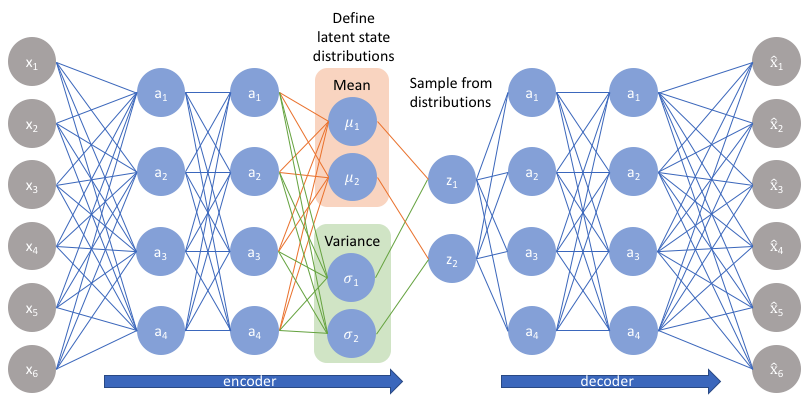
\includegraphics[width=0.8\textwidth]{tex/images/vae.png}
  \caption{Variational auto-encoder structure. Image taken from~\cite{JeremyJordan}.}\label{fig:vae}
\end{figure}


\ctparttext{
  \color{black}
  \begin{center}
    
  \end{center}
}
\part{Case study}

\chapter{Used frameworks}

Three different frameworks are used during this study, which are \texttt{InferPy}, \texttt{BayesPy} and \texttt{Scikit-Learn}. The first two are specifically designed to probabilistic modeling whereas the last one is a general machine learning library. For this reason, we are briefly describing the usage of the first two and only explaining the functions we are using on the last, but, before describing their usage, the study's file structure and used database are described.

Each study is made in a different file, available in both as a \texttt{Jupyter Notebook (.ipynb)} and \texttt{Python script (.py)} using the name format \texttt{[model]\_[framework]\_[database]}. Apart from these, there are three main auxiliary files:

\begin{itemize}
  \item \texttt{packages}: This file contains a list of the installed packages. These packages might be installed using \texttt{pip install -r packages}.
  \item \texttt{models.py}: In this \texttt{Python} file, all parametric and variational models from \texttt{InferPy} are defined. This includes PCA, NLPCA, VAE and Gaussian mixture.
  \item \texttt{functions.py}: In this file, all auxiliary functions are defined. The aim of these functions is either to make graphic representations or summarize the inference results.
\end{itemize}

Two different databases are used:
\begin{itemize}
  \item \texttt{Mnist}: a largely used dataset on a set of handwritten digits.
  \item \texttt{Breast Cancer Wisconsin}: characteristics of the cell nuclei present in breast mass.
\end{itemize}

\subsection{Mnist}

\texttt{Mnist} database (\cite{lecun-mnisthandwrittendigit-2010}) can be directly obtained through one of the used frameworks, \texttt{InferPy.data}. It consists of a set of \(70.000\)  handwritten digits, codified as \(28\times 28\) matrices where each position is the gray-scale value of the digit, in \([0,255]\)  (Figure~\ref{fig:mnist_example} shows an example of digits within the database). Given this, the observed data belongs to \([0, 255]^{784}\). Each sample is labeled with its corresponding digit.

\begin{figure}[h!]
    \centering
    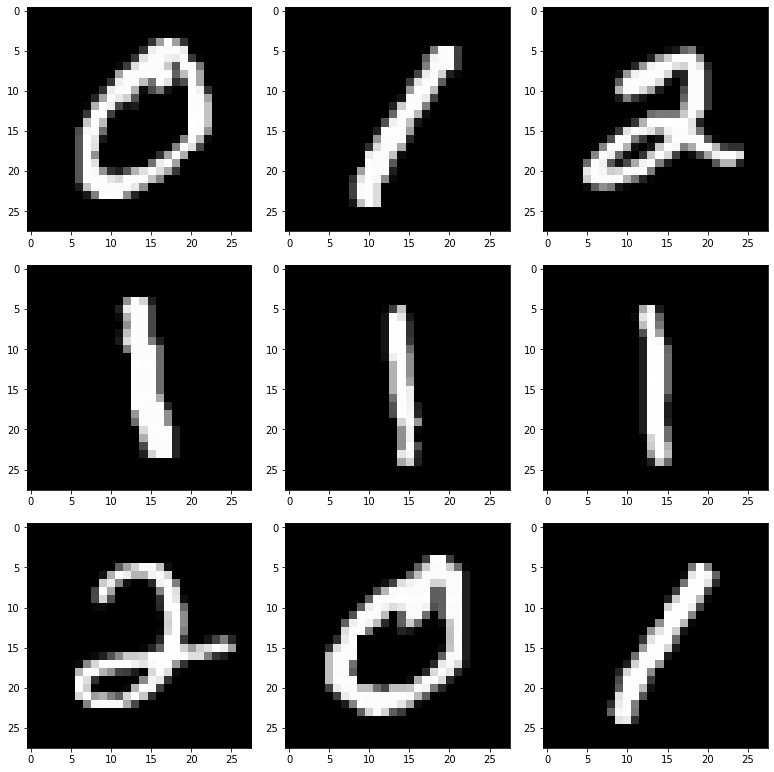
\includegraphics[width=0.35\textwidth]{tex/images/mnist.png}
    \caption{Mnist dataset example.}\label{fig:mnist_example}
  \end{figure}

Due to the size of the database, \(1000\) samples of digits \(1,4\) and \(7\) are used. These are loaded form \texttt{InferPy} directly:

\begin{minted}{python}
  mnist.load_data(num_instances=1000, digits=[1,4,7])
\end{minted}

Function \texttt{print\_class\_pie\_diagram} draws a class pie diagram of the given label set, in this case, their proportions are almost equal (Figure~\ref{fig:mnist_proportion}).

\begin{figure}
  \centering
  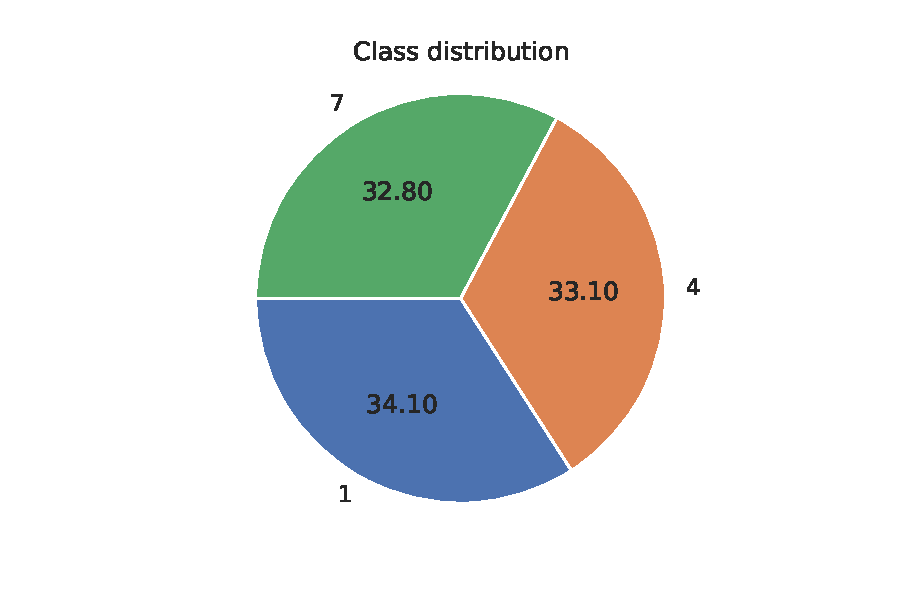
\includegraphics[width = 0.5\textwidth]{tex/images/mnist_proportion.pdf}
  \caption{Mnist class proportion between numbers \(1, 4\) and \(7\).}\label{fig:mnist_proportion}
\end{figure}

\subsection{Breast cancer Wisconsin}

\texttt{Breast cancer} database can be obtained from its \texttt{UCI} (\cite{DUA:2019}) repository \href{https://archive.ics.uci.edu/ml/datasets/Breast+Cancer+Wisconsin+(Diagnostic)}{link}. The database consists of \(569\) instances of \(30\) features of the cell nuclei present in breast mass. Among with each instance, an ID number and the diagnosis (\( M = \text{malign}\) and \(B = \text{benign}\)) are given. The given attributes are mean, standard error and worst (largest) value of all cells of the following features:
\begin{itemize}
  \item Radius: mean distance from the center to the perimeter.
  \item Texture: standard deviation of gray-scale values.
  \item Perimeter.
  \item Area.
  \item Smoothness: local variation in radius length.
  \item Compactness: \(perimeter^{2} / area - 1\).
  \item Concavity: severity of concave portions of the contour.
  \item Concave points: number of concave portions of the contour.
  \item Symmetry.
  \item Fractal dimension: a ratio comparing how detail in a fractal pattern changes with the scale of measurement.
\end{itemize}
All these features are coded with four significant digits.

In this database the class proportion is not balanced at all, Figure~\ref{fig:breast_proportion} shows a dominance of benign entries over the malign ones. Either way, this should not affect the obtained results.

\begin{figure}
  \centering
  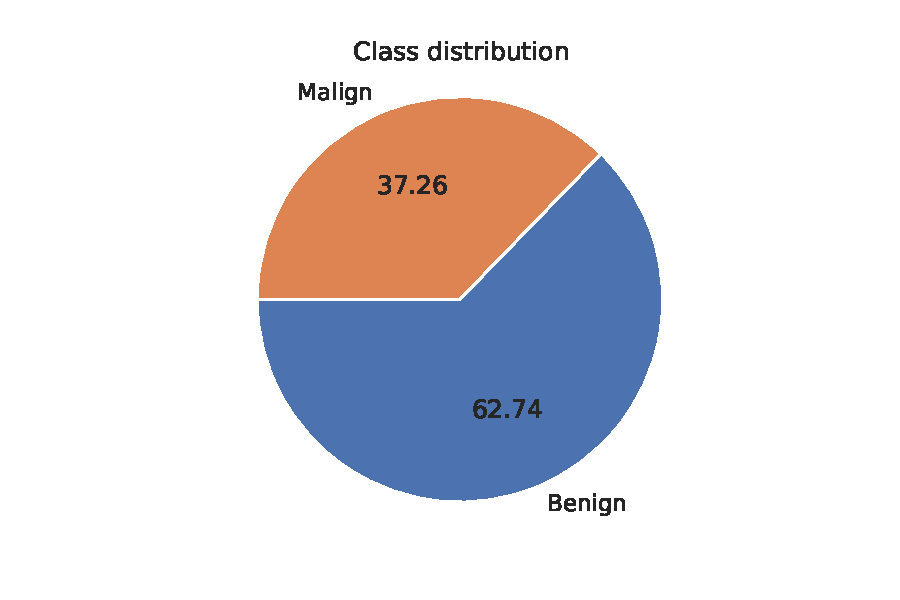
\includegraphics[width = 0.5\textwidth]{tex/images/breast_proportion.pdf}
  \caption{Breast cancer Wisconsin proportion of malign and benign labels.}\label{fig:breast_proportion}
\end{figure}

\section{InferPy}

\texttt{InferPy} (\cite{cozar2019inferpy}) is a high-level API written in \texttt{Python} inspired by \texttt{Keras} and run on top of \texttt{Tensorflow} and \texttt{Edward} for probabilistic modeling. It is focused on enabling probabilistic modeling, flexible data processing and scalable inference.

\begin{figure}[h!]
    \centering
    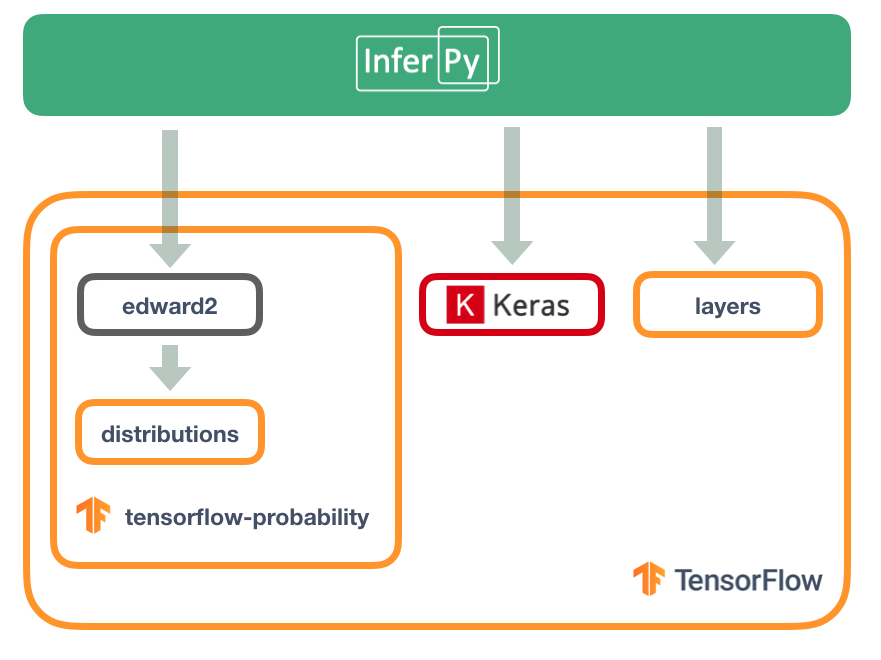
\includegraphics[width=0.7\textwidth]{tex/images/arch.png}
    \caption{InferPy architecture (\cite{cozar2019inferpy}).}
\end{figure}

\texttt{InferPy}'s main features are:
\begin{itemize}
  \item Allows to define probabilistic models whether they contain or not neural networks in a simple way.
  \item All models that can be defined using \texttt{Edward2} can also be defined in  \texttt{InferPy}, whose probability distributions are mainly inherited from \texttt{tensorflow-probability}.
  \item All the models parameters can be defined using the standard \texttt{Python} types (\texttt{Numpy} and \texttt{TensorFlow} compatibility).
  \item \texttt{InferPy} relies on top of \texttt{Edward}'s inference engine, therefore, it includes all the inference algorithms available in that package.
  \item As it uses \texttt{Edward} and \texttt{TensorFlow} as its inference engine, all the parallelization details are hidden to the user.
  \item The same code will run either in \textit{CPUs} or \textit{GPUs}.
\end{itemize}

\subsection{Installation}

\texttt{InferPy} has the following package requirements:
\begin{itemize}
    \item \texttt{Python} \( \geq\) 3.5 and \( < \) 3.8.
    \item \texttt{Tensorflow} \(\geq\)  1.12.1  and \( < \) 2.0.
    \item \texttt{Tensorflow-probability} 0.7.0.
    \item \texttt{NetworkX} \( \geq \) 2.2.0 and \( < \) 3.0.
\end{itemize}

\texttt{InferPy} is available at \texttt{Pip} and can be installed with the following command:

\begin{minted}{sh}
    pip install inferpy
\end{minted}

\subsection{Usage guide}

In all the following examples \texttt{InferPy} is imported as \texttt{inf}.

\texttt{Inferpy} requires that both the parametric \(P\) and the variational \(Q\) distribution are defined. In order to do so, models must be defined as \texttt{Python} functions inside a \texttt{@inf.probmodel} macro.

\begin{minted}{python}
    @inf.probmodel
    def model():
\end{minted}

Inside the model definition, both visible and hidden variables must be defined using the following syntax:

\begin{minted}[]{python}
    x =  inf.Normal(loc=tf.zeros([2]), scale=1, name="x")
\end{minted}

Distributions are imported from the package itself, as the case for \texttt{inf.Normal}. Distribution parameters must be passed during the definition, in this case, the mean (\texttt{loc}) and the standard deviation (\texttt{scale}) are used.

All variables must be given a name, variables with the same name in both the parametric and the variational model are considered the same variable. This is how both models communicate during the learning task. In the variational model, there must exist a parameter for each variable's parameter, in the case of the previous variable:
\begin{minted}[]{python}
    loc = inf.Parameter(tf.zeros([2]), name="x_loc")
    scale = tf.math.softplus(inf.Parameter(tf.ones([2]), name="x_scale"))
    x =  inf.Normal(loc, scale, name="x")
\end{minted}
Where a softplus function is used to avoid non-positive values.

If either the mean or the standard deviation are given as an array, a constant value on the other parameter would be interpreted as a constant array of the corresponding size. This is the case of the last definition where
\[
  X \sim \mathcal{N}_{2}(0,I).
\]

\texttt{InferPy} gives an explicit syntax for declaring a set of i.i.d random variables. Variables defined inside \texttt{with inf.datamodel(size)} are replicated the indicated number of times. This size can be omitted in the case of observations as it is calculated from the dataset at learning time.
\begin{minted}[]{python}
    with inf.datamodel():
        x = inf.Normal(tf.zeros([2]),1, name="x")
\end{minted}

When both models are defined and instantiated in a variable, we need to create an inference object, using a variational model as argument:
\begin{minted}{python}
    VI = inf.inference.VI(variational_model)
\end{minted}

By default, the inference is made using the machine learning technique \emph{gradient descent} which uses \(-\text{ELBO}\) as loss function (\href{https://github.com/PGM-Lab/InferPy/blob/master/inferpy/inference/variational/loss_functions/elbo.py}{source code}), notice that the ELBO takes values in \((-\infty, 0]\),  and uses \texttt{AdamOptimizer} (\cite{kingma2014adam}) from \texttt{TensorFlow}. An amount of \texttt{epochs} must be establish, which set the stop criteria to a of iterations to be done.

Given a training dataset \texttt{X\_train}, the model is trained indicating which set of observations corresponds to each observed variable using the following syntax:
\begin{minted}{python}
    model.fit({"x": X_train}, VI)
\end{minted}
Once the model is trained, a variable posterior can be taken as
\begin{minted}{python}
    model.posterior("z").parameters()
\end{minted}

\section{BayesPy}

\texttt{BayesPy} (\cite{BayesPy}) is a Bayesian inference \texttt{Python} package for modeling Bayesian networks and make inference. Currently, it only supports conjugate models in the exponential family as it only implements \emph{variational message passing algorithm} in contrast with \texttt{InferPy} that uses \emph{gradient descent}.

\subsection{Instalation}

The package can be installed using \texttt{pip install bayespy} and has the following requirements:
\begin{itemize}
  \item \texttt{NumPy} \(\geq\) 1.10.
  \item \texttt{SciPy} \(\geq\) 0.13.0.
  \item \texttt{matplotlib} \(\geq\) 1.2.
  \item \texttt{h5py}.
\end{itemize}

\subsection{Usage guide}

Three steps are needed to make Bayesian inference in \texttt{BayesPy}, firstly construct the model, secondly observe the data and lastly run the inference method.

Distributions are available at \texttt{BayesPy.nodes} and these nodes must be defined on \texttt{Python} objects. For example the following syntax
\begin{minted}{python}
  mu = nodes.Gaussian(np.zeros(2), np.identity(2), plates=(10))
\end{minted}
creates 10 i.i.d variables \(X_{1},\dots,X_{10}\)  such that
\[
  X_{n} \sim \mathcal{N}_{2}(0, I) \quad \forall n =1,\dots,10.
\]
Notice that the plate notation is done using a single parameter \texttt{plates}, in contrast with \texttt{InferPy} that used the syntax \texttt{with inf.datamodel()}.

When all nodes are created, the data must be observed using each node's \texttt{.observe()} method. Using the node's observations as argument.

The only inference method (VMP) is available at \texttt{bayespy.inference.VB} whose arguments must be all probabilistic nodes in the model, for example,
\begin{minted}{python}
  Q = VB(x, z, mu, Lambda, pi)
\end{minted}
creates the inference object of the Gaussian mixture model we studied. The inference method initializes the nodes variational prior automatically, either way, the user can decide how to initialize these values calling any of the following methods on the node itself:
\begin{itemize}
  \item \texttt{initialize\_from\_prior:} Uses the parent nodes to initialize the node. This is by default.
  \item \texttt{initialize\_from\_parameters:} Use the parameters given in the argument to initialize.
  \item \texttt{initialize\_from\_value:} Use the value given in the argument to initialize.
  \item \texttt{initialize\_from\_random:} Takes a random value for the variable.
\end{itemize}

The inference task is started using the method \texttt{.update()} from the \texttt{VB} object. By default the nodes are updated using the same order in they where passed when creating the object, to change that, a new order can be given as a argument.
\begin{minted}{python}
  Q.update(z, mu, Lambda, pi).
\end{minted}

Another possible arguments are the number of iterations (\texttt{repeat}) and the relative tolerance, i.e, distance of the ELBO between iterations (\texttt{tol}). After each iteration the value of the ELBO (\texttt{loglike}) is displayed.

\section{Scikit-Learn}

\texttt{Scikit-Learn} (\cite{scikit-learn}) is an open source library focused on providing machine learning tools, which include model fitting, selection and evaluation. From this library, we are using the \texttt{BayesianGaussianMixture} class which provides variational estimation of a Gaussian mixture model using the EM algorithm.
In the implementation of the algorithm, the variational distribution family is fixed as in Chapter~\ref{ch:gm}, for this reason, the \textbf{E-step}, which optimizes the variational distribution, only computes auxiliary values. Meanwhile, the \textbf{M-step} does optimize the parameters (hyper-parameters in this case), that is, the parameters of \(\bmu, \bLambda, \bz\) and \(\bpi\). This updates can be found in the class \href{https://github.com/scikit-learn/scikit-learn/blob/0fb307bf3/sklearn/mixture/_bayesian_mixture.py#L65}{source code}, and are equal to the ones we computed for the CAVI algorithm in Chapter~\ref{ch:gm}.

As this package is not specifically designed to make Bayesian inference, no nodes need to be defined as the model is internally handled. This being said, \texttt{BayesianGaussianMixture} models all decisions via its parameters:
\begin{itemize}
  \item \texttt{n\_components}: total amount of mixture components, default value is 1.
  \item \texttt{covariance\_type}: describes the type of covariance to use in the model. \texttt{full} means that each component has its own covariance matrix, \texttt{tied} means that all components have the same matrix, \texttt{diag} means that each component has its own covariance matrix but it must be diagonal and \texttt{spherical} means that each component has its own single variance value, i.e, diagonal matrix with the same value. The default value is \texttt{full}.
  \item \texttt{tol}: Tolerance threshold, 0.001 by default.
  \item \texttt{max\_iter}: Number of iterations to make. By default 100.
  \item \texttt{init\_params}: Handles the weights initialization, where \texttt{kmeans} and \texttt{random} are possible. By default K-means is used.
  \item \texttt{weight\_concentration\_prior\_type}: Describes how the weights prior is modeled. \texttt{dirichlet\_process} or \texttt{dirichlet\_distribution}. Where a Dirichlet process is an infinite-dimensional generalization of the Dirichlet distribution, used for infinite Gaussian Mixtures. This is used by default.
  \item \texttt{weight\_concentration\_prior}: Real value corresponding to each component weight value. By default equals \(1/n\_components\).
  \item \texttt{mean\_precision\_prior}: The precision prior of the mean distribution, by default 1.
  \item \texttt{mean\_prior}: The mean prior of the mean distribution, by default the mean of the dataset.
  \item \texttt{degrees\_of\_freedom\_prior}: Degrees of freedom of the Wishart distribution, by default the ammount of features of the data.
  \item \texttt{covariance\_prior}: Prior matrix of the Wishart distribution equals. By default it is initialized to the empirical covariance matrix.
\end{itemize}

The inference task is as simple as creating the Gaussian mixture object:
\begin{minted}{python}
  gm = BayesianGaussianMixture()
\end{minted}
Use the dataset to fit the model:
\begin{minted}{python}
  gm.fit(X)
\end{minted}

Once done, the posterior parameters can be inspected using the attributes \texttt{weights\_}, \texttt{means\_} and \texttt{precisions\_}. As many models in this package, the model can be used to predict a new input using \texttt{gm.predict(X)}. The probability of belonging to each component can be also computed using \texttt{gm.predict\_proba(X)}.


\chapter{Dimensionality Reduction}

In this section, the results obtained from using \texttt{InferPy} to achieve dimensionality reduction of the two given databases to a two-dimensional and a three-dimensional space are reviewed.


\section{Defined models}

The PCA model is defined with the following elements:
\begin{itemize}
  \item The set of i.i.d observed variables \(X_{1},\dots,X_{N}\).
  \item The hidden representation of each variable \(Z_{1}, \dots, Z_{N}\).
  \item A global hidden variable \(\bm{W}\) the linear transformation from one space to the other.
  \item Another global variable \( \delta \) that will allow the model to generate non-centered points.
\end{itemize}

The latent variables prior is a centered Gaussian and the data is supposed to be generated as
\[
     X_n \mid z_n, \bm{w}, \delta \sim \mathcal{N}(\bm{w}^T z_n + \delta, I)
\]
The considered noise value is therefore \(\sigma^{2} = 1\).

\begin{figure}[h!]
  \centering
  \begin{tikzpicture}[
    node distance=1cm and 0.5cm,
    mynode/.style={draw,circle,text width=0.6cm,align=center},
    param/.style={draw,text width=0.5cm,align=center}
    ]

    \node[mynode] (theta) {\(\bm{W}\)};
    \node[mynode, below left=of theta] (zn) {\(Z_{n}\)};
    \node[mynode, ,fill={rgb:black,1;white,2},below right=of theta] (xn) {\(X_{n}\)};
    \node[mynode, above right=of xn] (theta0) {\(\delta\)};


    \plate{} {(zn)(xn)} {\(n = 1\dots N\)}; %
    \path (theta) edge[-latex] (xn)
    (theta0) edge[-latex] (xn)
    (zn) edge[-latex] (xn)
    ;

  \end{tikzpicture}
  \caption{Non-centered Probabilistic PCA model. No noise considered.}
\end{figure}

This model is defined in \texttt{inferPy} as:
\begin{minted}{python}
  @inf.probmodel
  def pca(hidden_dim, observed_dim):
      w = inf.Normal(loc=tf.zeros([hidden_dim, observed_dim]), scale=1, name="w")
      delta = inf.Normal(loc=tf.zeros([observed_dim]), scale=1, name="delta")
      with inf.datamodel():
          z = inf.Normal(tf.zeros([hidden_dim]), 1, name="z")
          x = inf.Normal(z @ w + w0, 1, name="x")
        \end{minted}

The non-linear PCA model is defined using a two-layer neural network, to achieve this, four variables are defined \(\alpha_{0}, \alpha_{1}, \beta_{0}\) and \(\beta_{1}\). All of them following a Gaussian distribution \(\mathcal{N}(0, I)\). The networks output is then computed as

\begin{minted}{python}
  h = tf.nn.relu(z @ beta0 + alpha0)
  return h @ beta1 + alpha1
\end{minted}

This is done to show how \texttt{InferPy} allow networks can be modeled using variables. In the other hand, the variational auto-encoder model is defined using \texttt{Keras} integration with \texttt{InferPy}, so that both networks are defined as an \texttt{inf.layers.Sequential} object.

\section{Results}

\subsection{Mnist}

Firstly, due to the size of the original database, only \(1000\) samples of digits \(1,4\) and \(7\) are used. These are loaded form \texttt{InferPy} directly:

\begin{minted}{python}
  mnist.load_data(num_instances=1000, digits=[1,4,7])
\end{minted}

Function \texttt{print\_class\_pie\_diagram} draws a class pie diagram of the given label set, in this case, their proportions are almost equal (Figure~\ref{fig:mnist_proportion}).

\begin{figure}
  \centering
  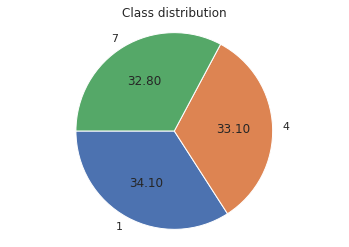
\includegraphics[width = 0.5\textwidth]{tex/images/mnist_proportion.png}
  \caption{Mnist class proportion between numbers \(1, 4\) and \(7\).}\label{fig:mnist_proportion}
\end{figure}

After the inference is done, a sample can be generated from the posterior of a latent variable \(Z\) using the input data:
\begin{minted}{python}
  sample = model.posterior("z", data={"x": X}).sample()
\end{minted}

The function \texttt{print\_posterior} might be used to draw 2D projections of a posterior sample. Results from the 2D reduction are shown in Figure~\ref{fig:mnist_posterior_2D}. In each of the graphics in that figure, projections to each of the learned latent variables are shown, leaving the diagonals to show the density of data-points in the corresponding variable.


\begin{figure}[ht]
  \centering
  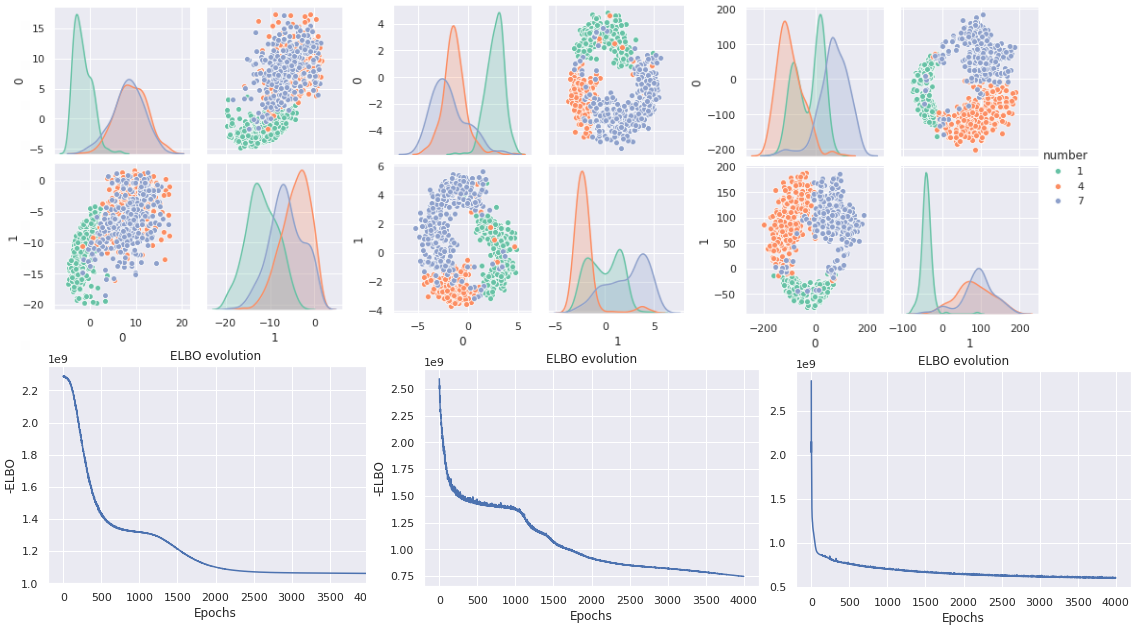
\includegraphics[width = 1\textwidth]{tex/images/mnist_2D.png}
  \caption{PCA, NLPCA and VAE posterior samples and loss functions (from left to right) from Mnist 2D reduction.}\label{fig:mnist_posterior_2D}
\end{figure}

For example in the first image, shown also in Figure~\ref{fig:mnist_pca_2D}, one may see (top left graph) that the first variable (\(0\)) strongly separates samples corresponding to \(1\) from the other samples, whereas the second variable (bottom right graph) (\(1\)) does not make such distinction.

\begin{figure}
  \centering
  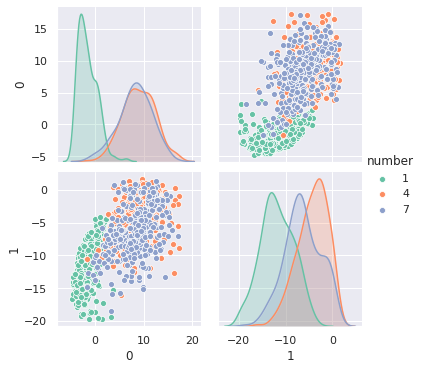
\includegraphics[width = 0.6\textwidth]{tex/images/mnist_pca_2D.png}
  \caption{Projections to each of the two learned variables in Mnist. Diagonals show density over the corresponding diagonal.}\label{fig:mnist_pca_2D}
\end{figure}

The generated representation of the NLPCA and VAE result in a similar ring form, where data samples seem separated between classes. One difference between both results is that the ring scale in the VAE case is bigger (\(200\) compared to \(5\)).

In the 3 cases the loss function (-ELBO) does decrease strongly during the first iteration and slowly during the last ones. This is accentuated in the VAE case (last plot).


In order to test the quality of the reduction, the fact that a good reduction must preserve class separability is used. To test this, the function \texttt{test\_separability} trains a \texttt{Support Vector Machine} from \texttt{Scikit-learn} over both the observed and the reduced space, displaying the score obtained in each one of these. Table~\ref{tab:mnist} shows the obtained results.


\begin{figure}
  \centering
  \begin{tabular}{ccc}
    \hline
    Model    & 2D reduction & 3D reduction \\\hline
    PCA      & 0.737 & 0.916\\
    NLPCA    & 0.947 & 0.969\\
    VAE      & 0.948 & 0.965\\
    \hline
    \hline
    Original data & 0.998 \\
    \hline
  \end{tabular}
  \caption{SVM score.}\label{tab:mnist}
\end{figure}

The three dimensional reduction results are shown in Figure~\ref{fig:mnist_posterior_3D}.

\begin{figure}[ht]
  \centering
  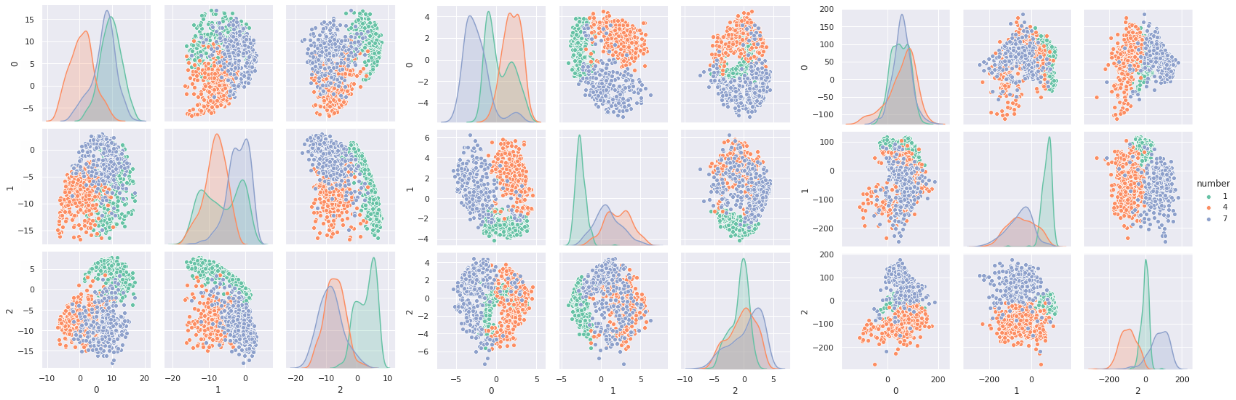
\includegraphics[width = 0.9\textwidth]{tex/images/mnist_3D.png}
  \caption{PCA, NLPCA and VAE posterior samples and loss functions from Mnist 3D reduction.}\label{fig:mnist_posterior_3D}
\end{figure}


\subsection{Breast Cancer Wisconsin}

Firstly, as the given identifier (\(\texttt{id}\)) is a non-predictive variable, it must be dropped from the dataset. Due to the relatively small size to the database, all entries are used in this case.

In this database the class proportion is not balanced at all, Figure~\ref{fig:breast_proportion} shows a dominance of benign entries over the malign ones. Either way, this should not affect the obtained results.

\begin{figure}
  \centering
  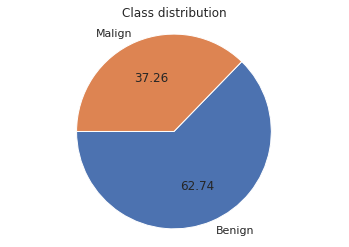
\includegraphics[width = 0.5\textwidth]{tex/images/breast_proportion.png}
  \caption{Breast cancer Wisconsin proportion of malign and benign labels.}\label{fig:breast_proportion}
\end{figure}

In this case, the obtained results from the two-dimensional (Figure~\ref{fig:breast_posterior_2D}) and the three-dimensional (Figure~\ref{fig:breast_posterior_3D}) are quite similar. Where the score table (Table~\ref{tab:breast}) shows very similar results in all cases. However, there are some details worth mentioning that make a difference with the obtained results in \texttt{Mnist}.



\begin{figure}[h]
  \centering
  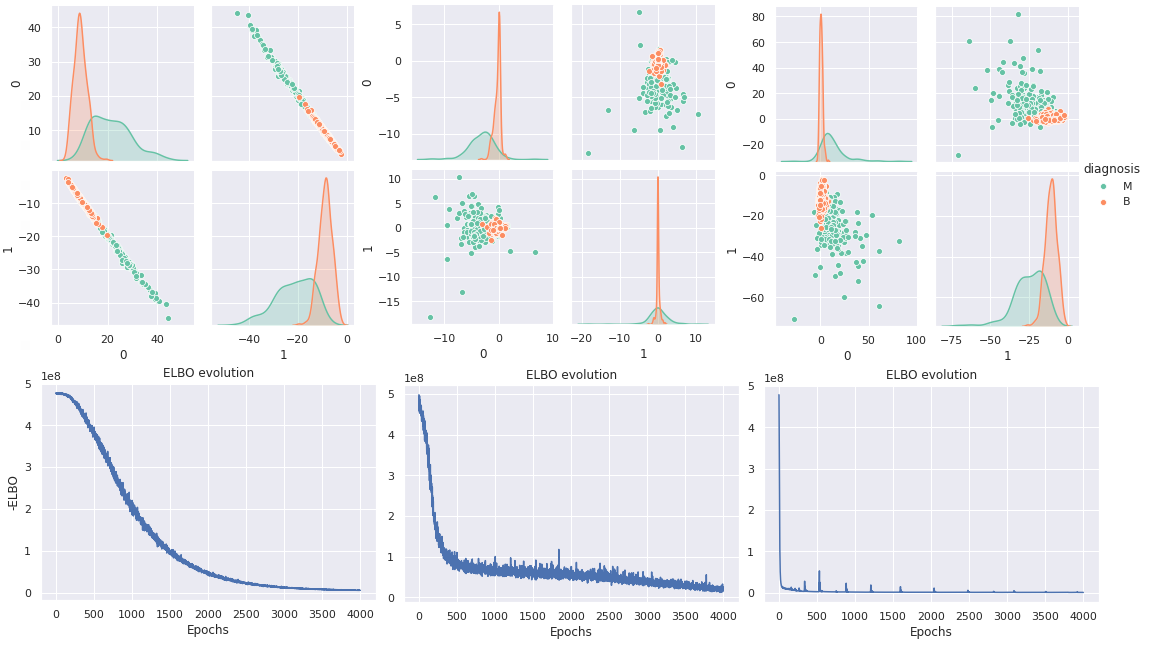
\includegraphics[width = 0.9\textwidth]{tex/images/breast_2D.png}
  \caption{PCA, NLPCA and VAE posterior samples and loss functions from Breast Cancer 2D reduction.}\label{fig:breast_posterior_2D}
\end{figure}

First of all, the results obtained from all models in this database show a highly sharp distribution on the benign entries and a more extended one on the malign one. Secondly, in both reductions, the probabilistic PCA model made a reduction where all the data-points resulted aligned, as a result, these two or three variables are highly correlated, which is not a desired outcome.

In this database, the obtained loss functions present greater oscillations compared to \texttt{Mnist}, which means that the learning task has encountered more local minimum compared to the other database.

\begin{figure}
  \centering
  \begin{tabular}{ccc}
    \hline
    Model    & 2D reduction & 3D reduction \\\hline
    PCA      & 0.9068 & 0.9103\\
    NLPCA    & 0.9121 & 0.9121\\
    VAE      & 0.9349 & 0.9209\\
    \hline
    \hline
    Original data & 0.9226 \\
    \hline
  \end{tabular}
  \caption{SVM score.}\label{tab:breast}
\end{figure}

It is worth mentioning that the separability has being increased (from \(0.9226\) to \(0.9349\)) after reducing to a two-dimensional space using a variational auto-encoder. This ensures that the given reduction does preserve the properties of the database.

There is no big difference between using a two or three dimension in this dataset.

\begin{figure}[ht]
  \centering
  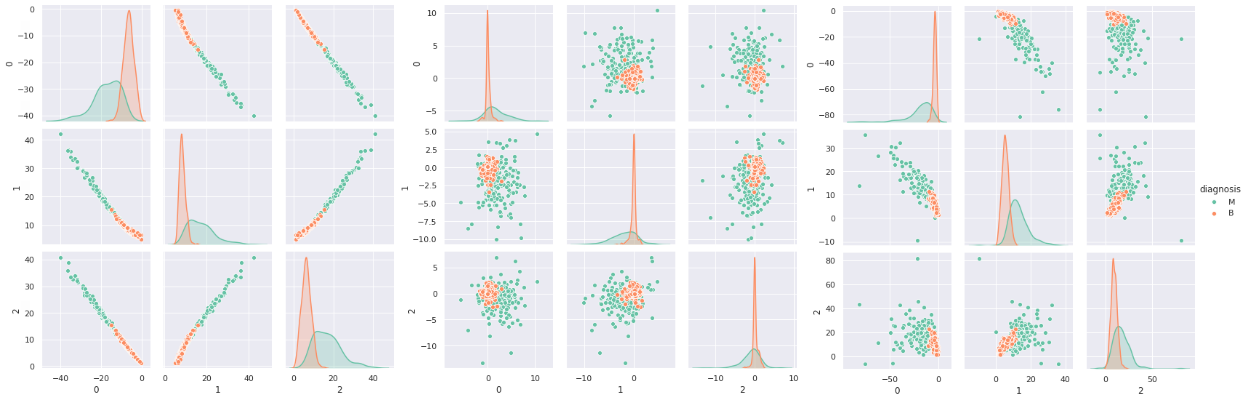
\includegraphics[width = 0.9\textwidth]{tex/images/breast_3D.png}
  \caption{PCA, NLPCA and VAE posterior samples and loss functions from Breast Cancer 3D reduction.}\label{fig:breast_posterior_3D}
\end{figure}



\chapter{Gaussian Mixture}

In this section, the obtained results from a Gaussian mixture training are reviewed. Two out of three frameworks are succesfully tested in this model.

In both frameworks \texttt{Breast Cancer} database is used with the main goal of learning a Gaussian mixture model, the original database and the one obtained via a dimensionality reduction. The latter is done using a variational auto-encoder with \texttt{InferPy}, showing that frameworks can be used together.

\section{InferPy}

Firstly, the Gaussian mixture cannot be directly modeled using \texttt{InferPy} due to the fact that \texttt{TensorFlow} \texttt{-Probability} name categorical variables as \texttt{NOT\_REPARAMETERIZED}, which, citing its documentation means that ``samples from the distribution are not fully reparameterized, and straight-through gradients are either partially unsupported or are not supported at all''. Unsuccessful attempts have being made using \texttt{MixtureGaussian} distribution available in \texttt{InferPy}, which encapsulates the mixture without needed explicit categorical variables. In this attempts, parameters that must remain positive reach negatives values even using a \texttt{softplus} filter, which makes inference not possible.

Adding a constant term to those parameters, such as, \(0.1\) in an attempt to keep them positive resulted in no learning errors but also no real results, where even the component weight parameter remained nearby its prior value on Breast Cancer database (where it should tend to \([0.63,\ 0.37]\)).


\section{Scikit-Learn}

Because of the high number of parameters, models are defined with \texttt{covariance\_type = ``diag''}, which means that all covariance matrix are diagonal. Using \texttt{``full''} covariance matrix would mean that two \(30 \times 30\) matrices might be learned from only \(569\) datapoints. Doing this reduction, the amount of covariance parameters is reduced to \(2\times 30 = 60\).

One of the parameters that can be easily studied when dealing with \(30\) parameters is the weight of each component:

\begin{minted}{python}
  print(gm.weights_)
\end{minted}

Which resulted in \([0.31003524\ 0.68996476]\) after the training and is more accurate than the prior value (\(0.5\) each).

\texttt{Scikit-Learn} allows to compute the posterior probability of belonging to each component by the usage of \texttt{gm.predict\_proba(points)}. This might be applied to each class, showing how it is distributed over the components, an ideal result would be that each of the classes is totally governed by each component. Function \texttt{plot\_mixture\_distplot} computes the posterior probabilities for each class, showing a density function fitting this results. Figure~\ref{fig:proba_ob} shows this density functions over the original dataset.

\begin{figure}[h!]
  \centering
  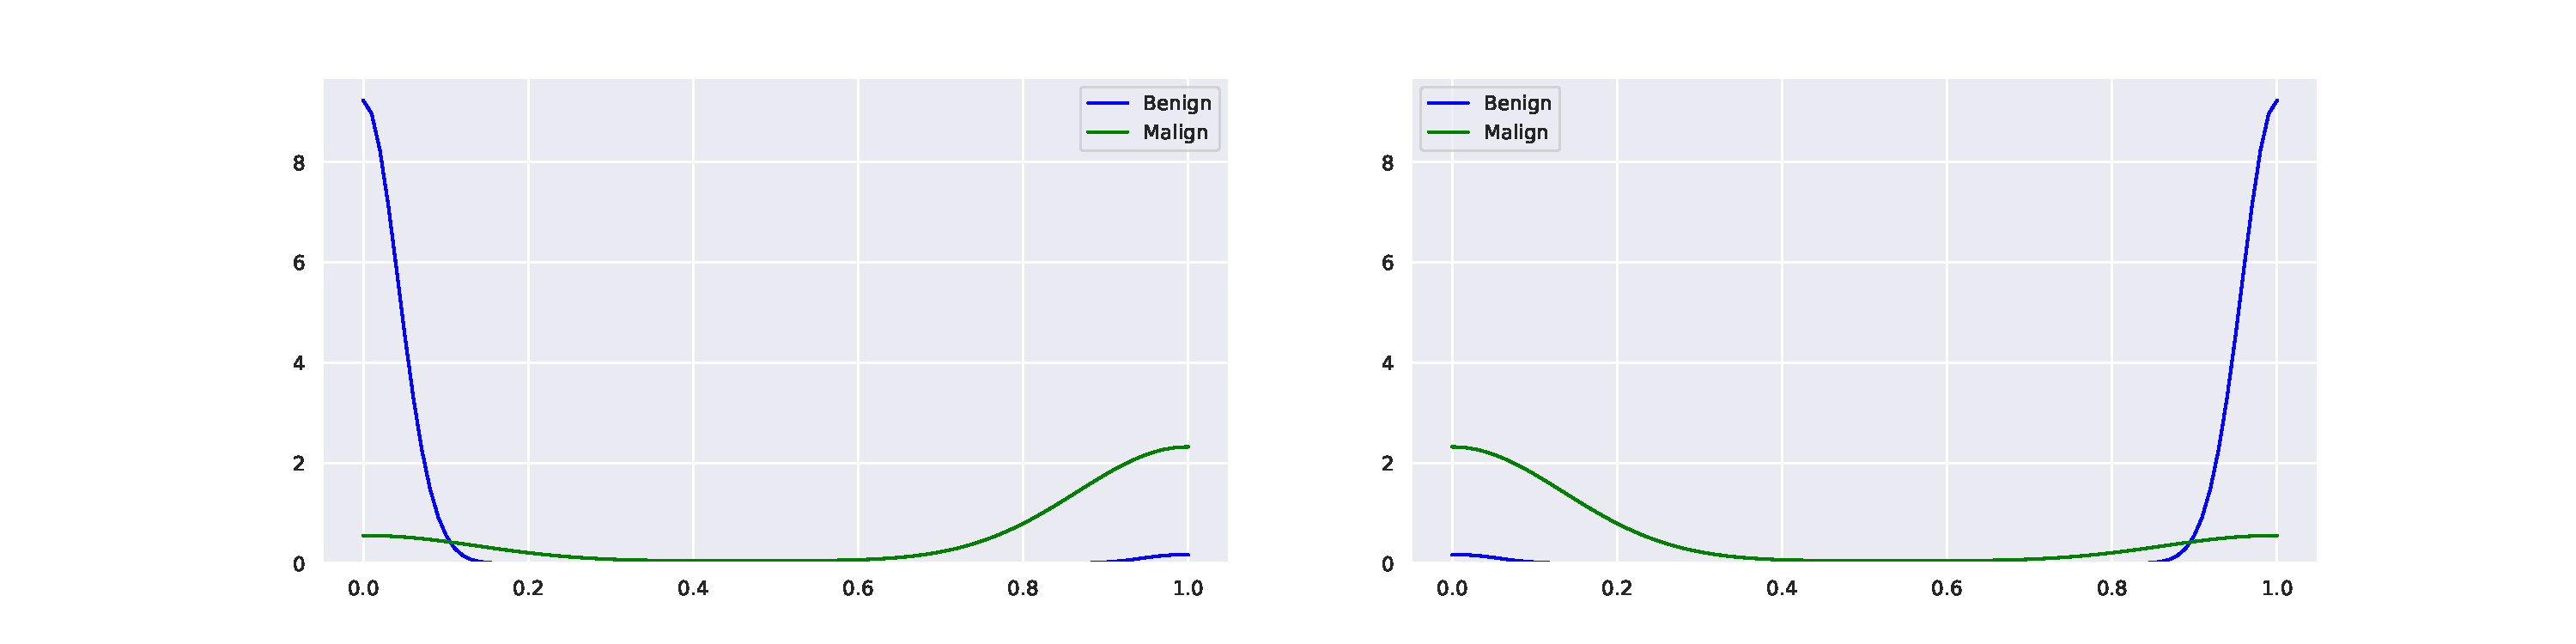
\includegraphics[width=0.9\textwidth]{tex/images/proba_observed.pdf}
  \caption{Component belonging density.}\label{fig:proba_ob}
\end{figure}

One may see that benign cases are almost completely modeled by the second component whereas the malign ones are more distributed but still modeled by the first component.

The dataset is now reduced to a three-dimensional representation using a variational auto-encoder, the dimensionality of the middle layer is \(100\) and \(4000\) epochs are used. The obtained reduction is shown in Figure~\ref{fig:vae_mix_breast}. The obtained component belonging densities are shown in
Figure~\ref{fig:proba_red} on the reduced space, showing a sharper density on the benign class compared to the original data, meaning that this class is better represented by the component in the reduced space.

\begin{figure}[h!]
    \centering
    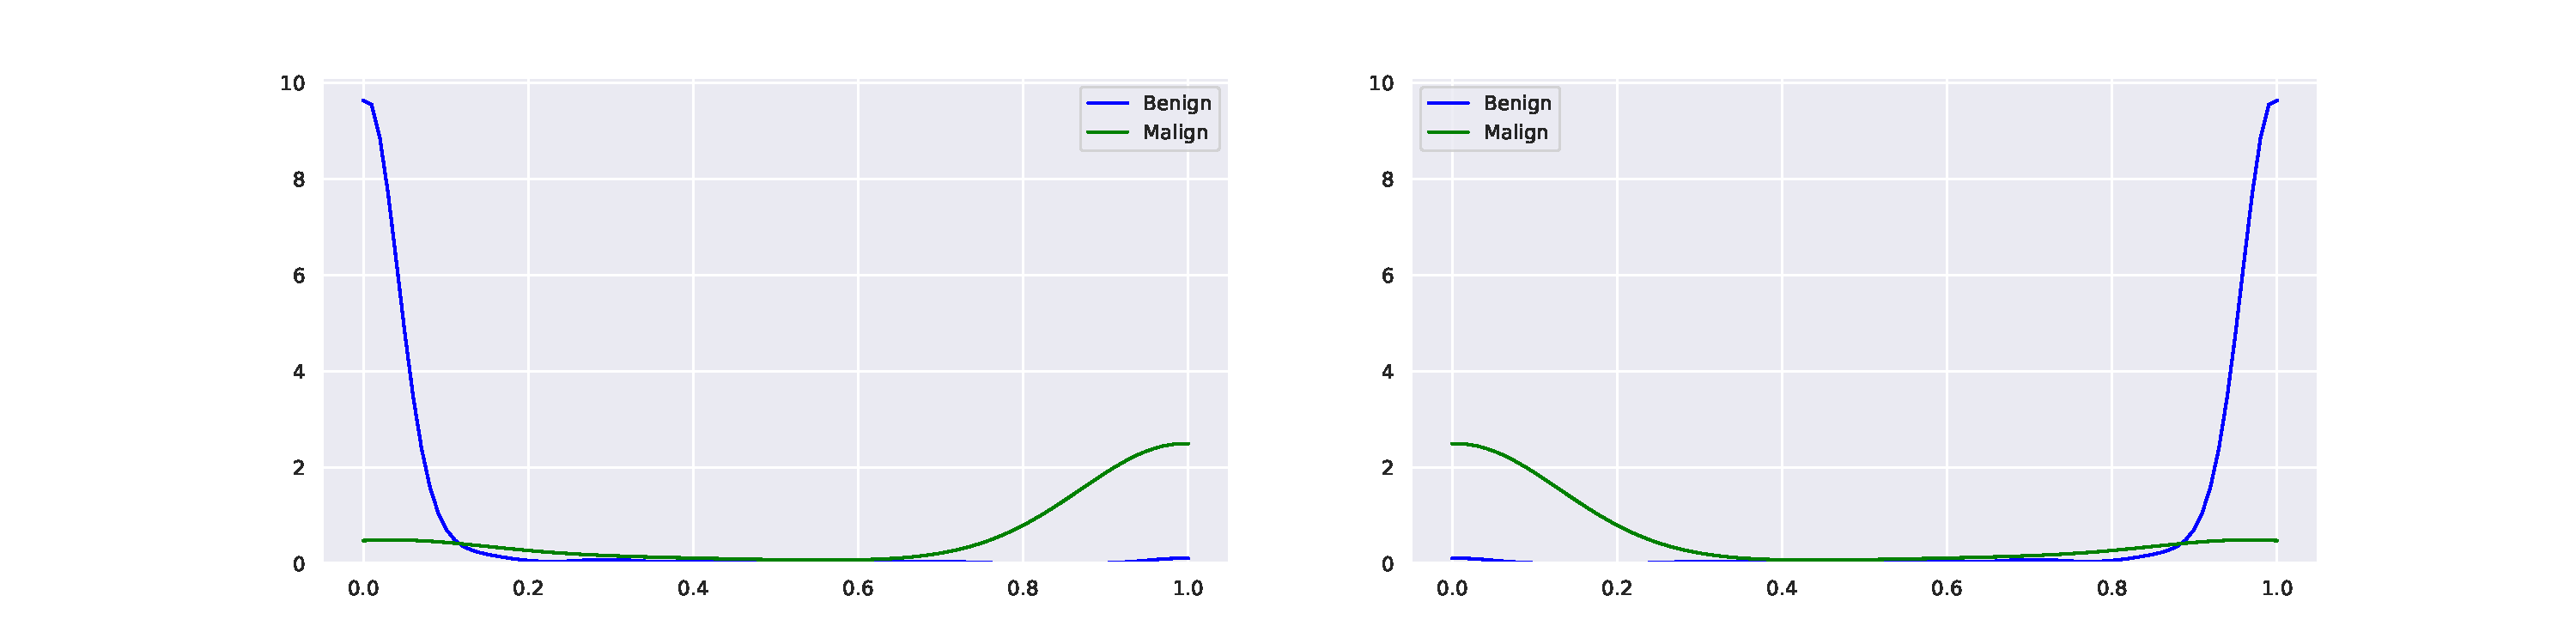
\includegraphics[width=0.9\textwidth]{tex/images/proba_reduced.pdf}
    \caption{Component belonging density in reduced data.}\label{fig:proba_red}
\end{figure}


\begin{figure}[h!]
  \centering
  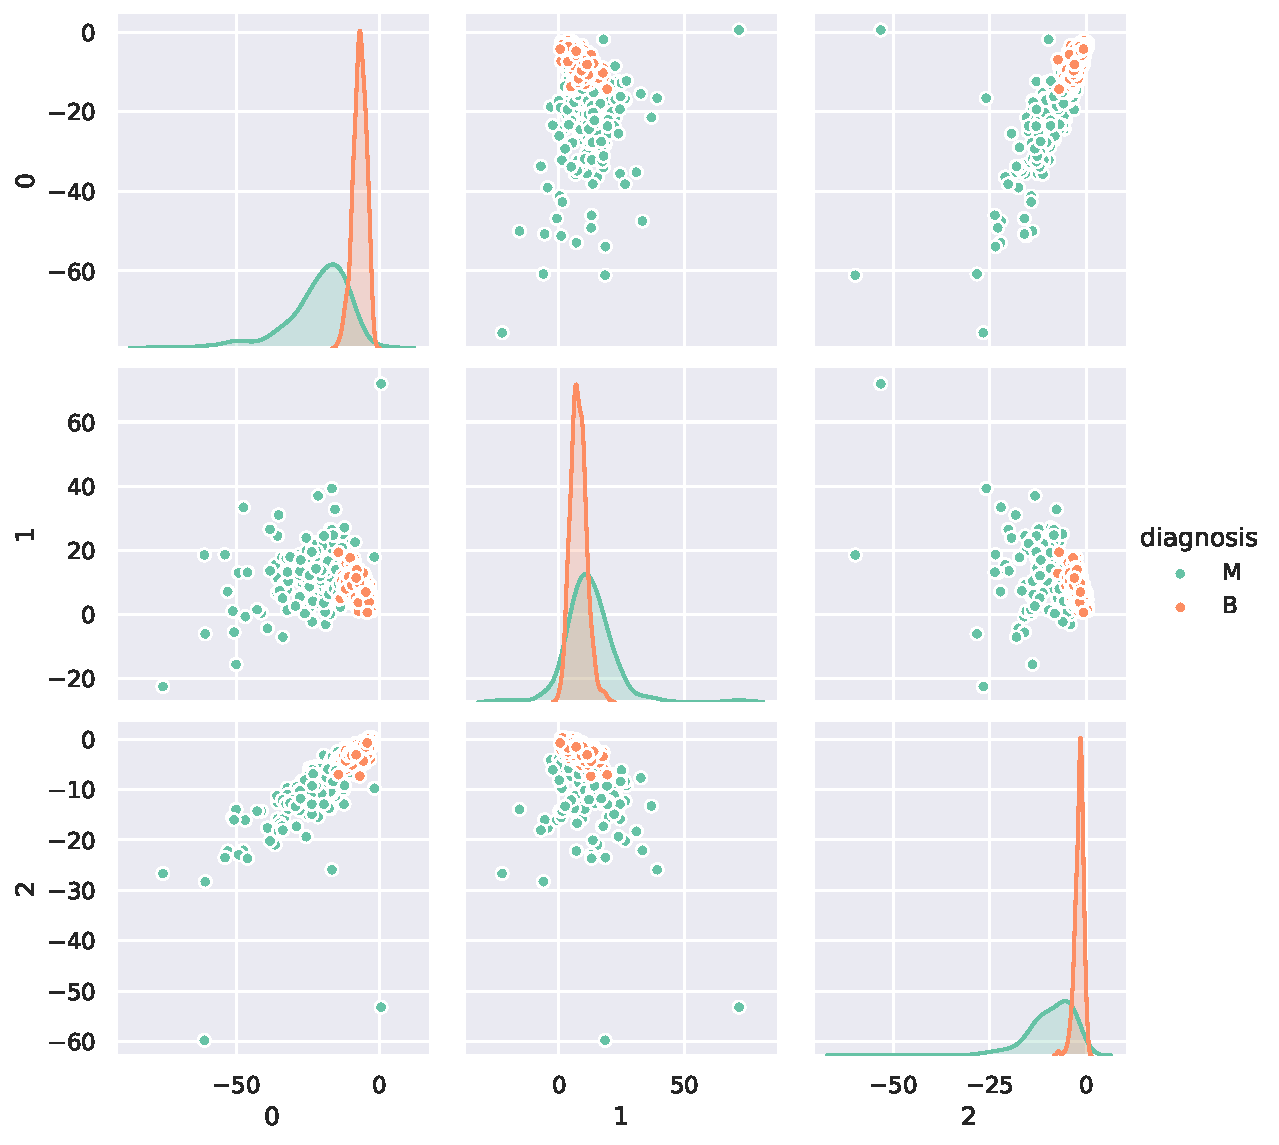
\includegraphics[width=0.9\textwidth]{tex/images/breast_vae_3D_mixture.pdf}
  \caption{Breast Cancer two-dimensional reduction representation. Reduction made trough a variational auto-encoder.}\label{fig:vae_mix_breast}
\end{figure}

As the representation is three-dimensional it is easy to compare other parameters as the mean value of each component, these are \([ 16.15134999,\  -3.88342216,\ -18.26021824]\) and \([7.25244497,\   1.90782194,\  -5.72329033]\). Using this values and Figure~\ref{fig:vae_mix_breast}, one may notice that the first component seeks to model the malign points and the second the benign ones.

\newpage
\section{BayesPy}

The \texttt{BayesPy} model can be easily created using the syntax explained before, the model parameters are initialized as
\begin{itemize}
  \item The means variable $\mu$ follows a centered normal distribution:
  $$\mu_k \sim \mathcal{N}_{data\_dim}(0,I).$$
  \item The precision variables $\Lambda$ follow a Wishart distribution with parameters:
  $$\Lambda_k \sim \mathcal{W}_{data\_dim}(data\_dim, I).$$
  \item The weights concentration variable follows a Dirichlet with parameter:
  $$ \pi \sim \text{Symmetric-Dirichlet}\Big(\frac{1}{n\_classes}\Big).$$
\end{itemize}

Which is coded as the following.
\begin{minted}{python}
    Lambda = nodes.Wishart(dim, np.identity(dim), plates=(n_components,))
    mu = nodes.Gaussian(np.zeros(dim), np.identity(dim), plates=(n_components,))
    pi = nodes.Dirichlet(np.ones(n_components)/n_components)
    z = nodes.Categorical(pi, plates=(n_samples,))
    x = nodes.Mixture(z, nodes.Gaussian, mu, Lambda)
\end{minted}

Due to the high number of attributes (784) in \texttt{Mnist} database, \texttt{BayesPy} is not able to handle the VMP algorithm with a great number of samples (it attempts to locate a matrix with shape \((n\_samples,\ n\_components,\ 784,\ 784)\)). For this reason, \texttt{Breast Cancer} is used.

The model is created with the same number of components as different classes (2) in an attempt to learn one Gaussian distribution for each class. After the inference task, \texttt{BayesPy} provides a way to inspect each variable posterior by simply printing the desired variable.

Variable moments are also accessible via each variable \texttt{u} parameter, given this, we may learn each data-point component belonging posterior, using \texttt{Z's} first moment.

The obtained results show a model that does not learn the two classes, despite that, almost all data-points belong to one of the components with high probability. The exact posterior for \(\bpi\) is \([6.5/570\  563.5/570]\). Furthermore, the component assignment variable posterior sets the benign class in the second component with probability \(1\), with a \(0\) variance between datapoints. Given this, no component belonging density function can be computed as we did with \texttt{Scikit-Learn}.

We may reduce the space to a two-dimensional one using a variational auto-encoder. In this case, the posterior for \(\bpi\) is \([0.61\ 0.39]\), which is similar to the real one (\([0.62\ 0.38]\)). This gives the intuition that the first component models the more common class (benign). This is confirmed using the component belonging densities (Figure~\ref{fig:proba_reduced_bayes}). These are similar to the ones obtained using \texttt{Scikit-Learn}.
 
\begin{figure}[h!]
  \centering
  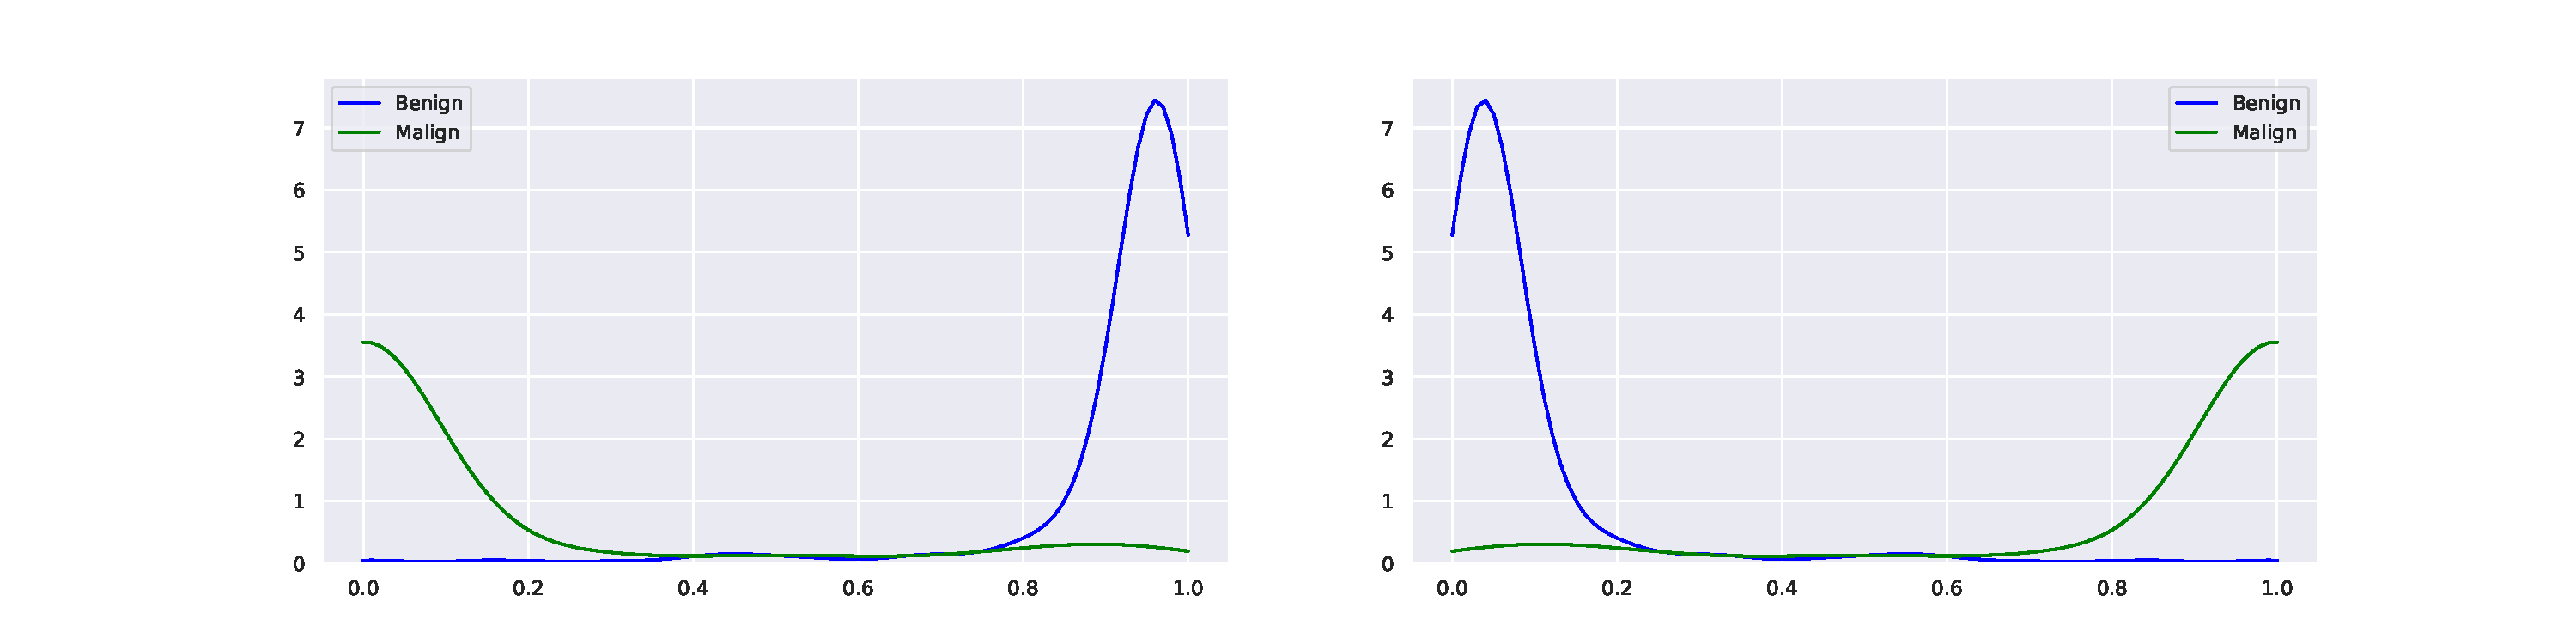
\includegraphics[width=0.9\textwidth]{tex/images/proba_reduced_bayes.pdf}
  \caption{Component belonging density in reduced data.}\label{fig:proba_reduced_bayes}
\end{figure}




\ctparttext{
  \color{black}
  \begin{center}

  \end{center}
}
\part*{\textsc{Annexes}}

\appendix
\chapter{Distributions in the exponential family}\label{ap:exp_fam}
\everymath{\displaystyle}
\renewcommand*{\arraystretch}{1.3}
  \begin{longtable}{|c|c|c|c|c| }
    \hline
    Distribution & Parameter set \(\btheta\) & Base measure \(h\) & Parameter function \(\bm{\eta}(\btheta)\) & Statistics \(\bm{T}(x)\) \\
    \hline
    Bernoulli & \(p\)  & \(1\)  & \(\log{\frac{p}{1 - p}}\) & \(x\) \\[5pt]
    Binomial & \(p\)  & \(\binom{n}{x}\) & \(\log{\frac{p}{1 - p}}\) & \(x\)  \\[5pt]
    Categorical & \(p_{1},\dots,p_{K}\) & \(1\) &
                                                  \(\begin{bmatrix}
                                                    \log p_{1}\\
                                                    \vdots\\
                                                    \log p_{K}
                                                  \end{bmatrix}\)
                 &
                                                  \(\begin{bmatrix}
                                                    [x=1]\\
                                                    \vdots\\
                                                    [x=k]
                                                  \end{bmatrix}\)\\[30pt]
    Gaussian & \(\mu, \sigma^{2}\) & \(\frac{1}{\sqrt{2\pi}}\) &
                                     \(\begin{bmatrix}
                                       \frac{\mu}{\sigma^2}\\
                                       -\frac{1}{2\sigma^{2}}
                                     \end{bmatrix}\)
                 &
                   \(\begin{bmatrix}
                     x\\
                     x^{2}
                   \end{bmatrix}\) \\[30pt]
    Beta & \(\alpha, \beta\) & \(\frac{1}{x(1-x)}\)
                                                               &
                                                                 \(\begin{bmatrix}
                                                                   \alpha \\
                                                                   \beta
                                                                 \end{bmatrix}\)
                 &
                   \(\begin{bmatrix}
                     \log x \\
                     \log (1-x)
                   \end{bmatrix}\) \\[30pt]
    Dirichlet & \(\alpha_{1},\dots,\alpha_{K}\) & \(1\) &
                                                  \(\begin{bmatrix}
                                                    \alpha_{1} - 1\\
                                                    \vdots\\
                                                    \alpha_{K} - 1
                                                  \end{bmatrix}\)
                 &
                                                  \(\begin{bmatrix}
                                                    \log x_{1}\\
                                                    \vdots\\
                                                    \log x_{K}
                                                  \end{bmatrix}\)\\
    \hline
  \end{longtable}


\chapter{Conjugate distributions}\label{ap:conj_distr}
In this appendix, examples of conjugate distributions and their conjugate priors are shown. In the following sections \(X\) will denote the given random variable and \(\bx = (X_{1},\dots,X_{N})\) a given set of observations.

\section*{Categorical and Dirichlet distributions}\label{ap:C-D}

\emph{The Dirichlet distribution is the conjugate prior of the Categorical distribution.}

Let \(X \sim Categorical(\btheta)\), where \(X\) takes values in \(\{1,\dots,I\}\) and \(\btheta = (\theta_{1},\dots,\theta_{I})\). The parameter follows a Dirichlet distribution \(\btheta \sim Dirichlet(\bm{u})\),
\[
  P(\bx \mid \btheta) = \prod_{i=1}^{I}\theta_{i}^{\sum_{n} \mathbb{I}[x_{n}=i]} \quad \text{and} \quad P(\btheta) = \frac{1}{B(\bm{u})}\prod_{i=1}^{I}\theta_{i}^{u_{i}-1}.
\]
The posterior is therefore,
\[
  P(\btheta \mid \bx) = \frac{P(\btheta)P(\bx \mid \btheta)}{P(x)} = \frac{1}{P(\bx)B(\bm{u})}\prod_{i=1}^{I}\theta_{i}^{u_{i}-1 + \sum_{n} \mathbb{I}[x_{n}=i]}
\]
Naming \(\bm{c} = \big(\sum_{n}\mathbb{I}[x_{n}=1], \dots, \sum_{n}\mathbb{I}[x_{n}=N]\big)\),
and given
\[
  \int_{\btheta}P(\btheta \mid \bx) = 1 \implies \int_{\btheta}\prod_{i=1}^{I}\theta_{i}^{u_{i} + c_{i} - 1} = B(\bm{u} + \bm{c}) = B(\bm{u})P(\bx).
\]
The posterior distribution follows a Dirichlet distribution with
\[
  \btheta \mid \bx \sim Dirichlet(\bm{c} + \bm{u}).
\]
A particular case would be using a Binomial distribution for the variable and a Beta distribution for the parameter. In short, \emph{the Beta distribution is the conjugate prior of the Binomial distribution.}

\section*{Gaussian and Wishart distributions}

\emph{The Wishart distribution is the conjugate prior of the Gaussian distribution with known mean and unknown precision.}

Let \(X \sim \mathcal{N}(\bmu, \bLambda)\), where \(\bmu\) is the mean vector and \(\bLambda\) the \(p \times p\)  precision matrix. The parameter follows a Wishart distribution as
\[
  \bLambda \sim \mathcal{W}(\nu, \bm{V}).
\]
Given \(N\) observations of the variable and \(\bx =(x_{1},\dots, x_{N})\). The density functions are
\[
  \begin{aligned}
    P(\bx \mid \bLambda) &= \frac{|\bLambda|^{N/2}}{{(2\pi^{k})}^{N/2}}\exp \Big( -\frac{1}{2}\sum_{n=1}^{N}{(x_{n} - \bmu)}^{T}\bLambda(x_{n} - \bmu) \Big)\\
    P(\bLambda) &= \frac{1}{2^{\nu p/2} |\bm{V}|^{\nu/2} \Gamma_{p}(\nu/2)}|\bLambda|^{(\nu-p-1)/2}e^{-(1/2)tr(\bm{V}^{-1}\bLambda)},
  \end{aligned}
\]
The prior distribution can be seen as proportional to
\[
  P(\bLambda) \propto |\bLambda|^{\frac{\nu-p-1}{2}} \exp \Big({-\frac{1}{2}tr(\bm{V}^{-1}\bLambda)}\Big),
\]
where the rest comes form normalization.
The posterior is then
\[
  \begin{aligned}
    P(\bLambda \mid x) &= \frac{1}{ {(2\pi^{k})}^{N/2}}|\bLambda|^{\frac{\nu+N-p-1}{2}} \exp \Big( -\frac{1}{2} \big(tr(\bm{V}^{-1}\bLambda) + \sum_{n=1}^{N}{(x_{n} - \bmu)}^{T}\bLambda(x_{n} - \bmu)\big) \Big)\\
    &= \frac{1}{ {(2\pi^{k})}^{N/2}}|\bLambda|^{\frac{\nu+N-p-1}{2}} \exp \Big( -\frac{1}{2} \big( tr(\bm{V}^{-1}\bLambda) + \sum_{n=1}^{N}tr({(x_{n} - \bmu)}^{T}\bLambda(x_{n} - \bmu))\big) \Big)\\
    &= \frac{1}{ {(2\pi^{k})}^{N/2}}|\bLambda|^{\frac{\nu+N-p-1}{2}} \exp \Big( -\frac{1}{2} \big( tr(\bm{V}^{-1}\bLambda) + \sum_{n=1}^{N}tr ((x_{n} - \bmu){(x_{n} - \bmu)}^{T}\bLambda)\big) \Big)\\
    &= \frac{1}{ {(2\pi^{k})}^{N/2}}|\bLambda|^{\frac{\nu+N-p-1}{2}} \exp \Big( -\frac{1}{2} \big( tr ( \bm{V}^{-1} +  \sum_{n=1}^{N}(x_{n} - \bmu){(x_{n} - \bmu)}^{T})\bLambda\big) \Big).
  \end{aligned}
\]
Where the property \(tr(ABC) = tr(BCA) = tr(CAB)\) is used. In conclusion, the posterior follows a Wishart distribution
\[
  \bLambda \mid \bx \sim \mathcal{W}\bigg(\nu + N, {\Big(\bm{V}^{-1} +  \sum_{n=1}^{N}(x_{n} - \bmu){(x_{n} - \bmu)}^{T}\Big)}^{-1}\bigg).
\]

\section*{Gaussian and Gaussian-Wishart distributions}\label{ap:G-GW}

\emph{The Gaussian-Wishart distribution is the conjugate prior of the Gaussian distribution with unknown mean and precision.}


Let \(X \sim \mathcal{N}(\bmu, \bLambda)\), where \(\bmu\) is the mean vector and \(\bLambda\) the \(p \times p\)  precision matrix. These parameters follow a Gaussian-Wishart distribution as
\[
  (\bmu, \bLambda) \sim \mathcal{N}\mathcal{W}(\bmu_{0}, {(\beta_{0}\bLambda)}^{-1}, \nu, \bm{V}).
\]
Given \(N\) observations of the variable and \(\bx =(x_{1},\dots, x_{N})\). The density functions are proportional to
\[
  \begin{aligned}
    P(\bx \mid \bmu, \bLambda) &\propto |\bLambda|^{\frac{N}{2}}\exp \Big( -\frac{1}{2}\sum_{n=1}^{N}{(x_{n} - \bmu)}^{T}\bLambda(x_{n} - \bmu) \Big),\\
    P(\bLambda) &\propto |\bLambda|^{\frac{\nu-p-1}{2}}\exp \Big(-\frac{1}{2}tr(\bm{V}^{-1}\bLambda)\Big),\\
    P(\bmu \mid \bLambda) &\propto |\bLambda|^{\frac{1}{2}} \exp \Big( -\frac{1}{2}(\bmu - \bmu_{0})^{T}(\beta_{0}\bLambda)(\bmu-\bmu_{0}) \Big).
  \end{aligned}
\]
The joint prior is proportional to
\[
  P(\bmu, \bLambda) \propto |\bLambda|^{\frac{1}{2}}|\bLambda|^{\frac{\nu-p-1}{2}}\exp \Big(-\frac{1}{2}tr(\bm{V}^{-1}\bLambda) -\frac{1}{2}(\bmu - \bmu_{0})^{T}(\beta_{0}\bLambda)(\bmu-\bmu_{0}) \Big).
\]
The posterior is then
\[
  P(\bmu, \bLambda \mid \bx) \propto P(\bx \mid \bmu, \bLambda)P(\bmu, \bLambda) = P(\bx \mid \bmu, \bLambda)P(\bmu \mid \bLambda) P(\bLambda).
\]
\[
  P(\bmu, \bLambda \mid \bx) \propto |\bLambda|^{\frac{\nu + N - p}{2}} \exp -\frac{1}{2}\Big( tr(\bV^{-1}\bLambda) + (\bmu - \bmu_{0})^{T} (\beta_{0}\bLambda)(\bmu - \bmu_{0}) + \sum_{n=1}^{N}(x_{n} - \bmu)^{T}\bLambda(x_{n}- \bmu)  \Big)
\]
As the Gaussian-Wishart distribution has \(\bLambda^{\frac{1}{2}}\) as a constant factor, the posterior's degrees of freedom \(\nu'\) is calculated using:
\[
  |\bLambda|^{\frac{\nu - p + N}{2}} = |\bLambda|^{\frac{\nu - p + N-1}{2}} |\bLambda|^{\frac{1}{2}}  \implies \nu' = \nu + N.
\]
Using the factors that surround \(\bLambda\) inside the exponential term, the new scale parameter \(\beta_{0}'\) is:
\[
  \bmu^{T}\beta_{0}\bLambda\bmu + N\bmu^{T}\bLambda\bmu = \bmu^{T}((\beta_{0} + N)\bLambda)\bmu \implies \beta_{0}' = \beta_{0} + N.
\]
The mean parameter comes from the updated term from \(2\bmu^{T}\beta_{0}\bLambda\bmu_{0}\), which is
\[
  2\bmu^{T}\beta_{0}'\bLambda\bmu_{0}' = 2\bmu^{T}(\bLambda N \bar{\bx} + \beta_{0}\bLambda\bmu_{0}) \implies \bmu_{0}' = \frac{1}{\beta_{0}'}(N\bar{\bx} + \beta_{0}\bmu_{0}).
\]
Where
\[
  \bar{\bx} = \frac{1}{N}\sum_{n=1}^{N}x_{n}.
\]
The updated scale matrix \(\bV'\) comes from computing the new trace value, adding to it any one dimensional term multiplied by \(\bLambda\).
\[
  \begin{aligned}
    tr(\bV'^{-1} \bLambda) &= tr(\bV^{-1}\bLambda + \sum_{n=1}^{N}(x_{n} - \bar{\bx})(x_{n} - \bar{\bx})^{T}\bLambda + \beta_{0}(\bar{\bx} - \bmu_{0})(\bar{\bx} - \bmu_{0})^{T}\bLambda\\
    &\quad+ (N - \beta_{0})\bar{\bx}\bar{\bx}^{T}\bLambda + 2\beta_{0}\bar{\bx}\mu_{0}^{T}\bLambda).
  \end{aligned}
\]
Then,
\[
  \bV'^{-1} = \Big(\bV^{-1} + \sum_{n=1}^{N}(x_{n} - \bar{\bx})(x_{n} - \bar{\bx})^{T} + \frac{\beta_{0}N}{\beta_{0} + N}(\bar{\bx} - \bmu_{0})(\bar{\bx} - \bmu_{0})^{T}\Big).
\]
As a result, the posterior follows a Gaussian-Wishart distribution
\[
  (\bmu, \bLambda \mid \bx) \sim \mathcal{N}\mathcal{W}(\bmu_{0}', (\beta_{0}'\bLambda)^{-1}, \nu', \bV').
\]



\addtocontents{toc}{\vspace{1\baselineskip}}
\clearpage

\printglossary[title={\textsc{notation}}]
\glsaddallunused

\clearpage
\nocite{*}
\bibliographystyle{authordate1}
\bibliography{tex/refs}
\end{document}
